% ============================================================================
%  Modelo completo del Segway con patas extensibles
%  Documento maestro: ata los cuatro PDF que ya existian y agrega los capitulos
%  del pendulo invertido, el motor, el LQR y Simulink.
%
%  Compilar DOS veces (por el indice) desde esta carpeta:
%     pdflatex -interaction=nonstopmode modelo_del_segway.tex
%  Requiere pdfpages y tcolorbox.
% ============================================================================
\documentclass[11pt,a4paper]{report}
\usepackage[utf8]{inputenc}
\usepackage[T1]{fontenc}
\usepackage[spanish,es-noshorthands]{babel}
\usepackage[margin=2.3cm]{geometry}
\usepackage{amsmath,amssymb}
\usepackage{graphicx}
\usepackage{booktabs}
\usepackage{xcolor}
\usepackage{tcolorbox}
\usepackage{pdfpages}
\usepackage{enumitem}
\usepackage{caption}
\usepackage[colorlinks=true,linkcolor=blue!50!black,urlcolor=blue!50!black,
            citecolor=blue!50!black]{hyperref}

\graphicspath{{../modelado/}{../modelado/cinematica/}{../modelado/dcl/}%
              {../modelado/dinamica/}{../modelado/geometria/}%
              {../modelado/ajuste/}%
              {../modelado/planta/pendulo_invertido/}%
              {../modelado/planta/pendulo_invertido/diagramas/}%
              {../simulacion/pendulo_invertido/resultados/}%
              {../simulacion/segway_completo/resultados/}%
              {../simulacion/segway_ajustado/resultados/}%
              {../simulacion/escalon/resultados/}%
              {../simulacion/escalon/resultados/un_escalon/}%
              {../simulacion/escalon/resultados/escalera_real/}%
              {../simulacion/escalon/resultados/pruebas/}%
              {../firmware/docs/}%
              {../Aplicacion/capturas/}%
              {../Aplicacion/diagramas/}}

\setlength{\parskip}{5pt}
\setlength{\parindent}{0pt}
\captionsetup{font=small,labelfont=bf}

\definecolor{azulp}{RGB}{31,95,168}
\definecolor{verdep}{RGB}{27,94,32}
\definecolor{rojop}{RGB}{198,40,40}
\definecolor{naranjap}{RGB}{217,83,30}

\newtcolorbox{idea}{colback=azulp!6,colframe=azulp,boxrule=0.9pt,
  left=7pt,right=7pt,top=6pt,bottom=6pt,arc=2pt,
  fonttitle=\bfseries,title=La idea}
\newtcolorbox{ojo}{colback=rojop!5,colframe=rojop,boxrule=0.9pt,
  left=7pt,right=7pt,top=6pt,bottom=6pt,arc=2pt,
  fonttitle=\bfseries,title=Ojo con esto}
\newtcolorbox{medido}{colback=verdep!5,colframe=verdep,boxrule=0.9pt,
  left=7pt,right=7pt,top=6pt,bottom=6pt,arc=2pt,
  fonttitle=\bfseries,title=Lo que está medido y lo que no}

\newcommand{\dd}{\mathrm{d}}
\newcommand{\ud}[1]{\,\mathrm{#1}}

\title{\vspace{-1.5cm}\Huge Informe Técnico Final: Segway con patas extensibles\\[10pt]
\large Del modelado físico y el diseño mecatrónico a la identificación experimental\\
y el descenso autónomo de escaleras\\[18pt]
\normalsize Memoria técnica integral: geometría, cinemática, dinámica de Lagrange, control LQR,\\
Simulink, diseño mecánico CAD, electrónica y PCB, firmware ESP-IDF, ajuste con el robot real\\
y optimización de maniobras con algoritmos genéticos}
\author{Grupo 4 --- Robótica II, Facultad de Ingeniería, UNCUYO\\[4pt]
\small Joaquín Calderón \quad\textbullet\quad Francisco Castel \quad\textbullet\quad Matías Armani}
\date{7 de noviembre de 2026}

\begin{document}
\maketitle

\begin{idea}
Este documento es la memoria técnica completa del proyecto. Explica, de abajo hacia arriba,
cómo se concibió, modeló, dimensionó, fabricó, programó y ensayó el robot, y por qué cada
decisión ingenieril es como es. No supone que el lector haya seguido el proyecto: los
capítulos principales desarrollan la física, la arquitectura y la validación experimental
sobre el prototipo construido, mientras que los apéndices conservan las deducciones
algebraicas completas y la documentación constructiva de las placas electrónicas.
\end{idea}

\vspace{4pt}
{\large\bfseries Cómo leer este informe}

\begin{center}
\begin{tabular}{@{}p{5.2cm}p{9.5cm}@{}}
\toprule
\textbf{Si querés\ldots} & \textbf{andá a\ldots} \\
\midrule
entender el robot y su física en diez minutos & capítulos \ref{cap:mapa2} y \ref{cap:pend} \\
dimensionar los servos y las cargas de impacto & capítulo \ref{cap:din} y apéndices \ref{ap:dcl} y \ref{ap:dinres} \\
entender los motores, la adherencia y el LQR & capítulos \ref{cap:motor} y \ref{cap:lqr} \\
correr y auditar el banco en Simulink & capítulo \ref{cap:simulink} \\
analizar el acople al mover las patas en vivo & capítulo \ref{cap:patasmov} \\
ver el diseño mecánico en CAD y el chasis final & capítulo \ref{cap:mec} \\
revisar la electrónica, protecciones y PCB v0.7 & capítulo \ref{cap:elec} y apéndice \ref{ap:pcb} \\
estudiar el firmware en tiempo real y la HMI/Joystick & capítulo \ref{cap:fw} \\
comparar la teoría contra las mediciones del robot & capítulo \ref{cap:ajuste} \\
analizar la bajada de escalón y escalera (algoritmo genético) & capítulo \ref{cap:escalon} \\
ver las deducciones algebraicas paso a paso & apéndices \ref{ap:cin} a \ref{ap:dinapo} \\
\bottomrule
\end{tabular}
\end{center}

Cada capítulo arranca con un recuadro azul con la idea en una o dos frases. Los recuadros
rojos marcan trampas donde ya nos equivocamos una vez, y los verdes separan lo medido de lo
supuesto, que en este proyecto es la distinción más importante de todas.

\tableofcontents

% ===========================================================================
\chapter{El mapa: qué hay que modelar y por qué}
% ===========================================================================

\section{Qué es el robot}

Un Segway con dos ruedas y, entre cada rueda y la cabina, una \textbf{pata extensible}: un
mecanismo de cuatro barras movido por un servo, que sube y baja el cuerpo. O sea, dos cosas
que a primera vista no se parecen en nada:

\begin{itemize}[leftmargin=1.5em]
\item un \textbf{péndulo invertido sobre ruedas}, que se cae solo y hay que sostenerlo
      moviendo las ruedas;
\item dos \textbf{patas} de un grado de libertad, que cambian la altura del cuerpo.
\end{itemize}

\section{Por qué hacen falta dos modelos y no uno}

Porque son dos problemas con escalas de tiempo distintas, y eso permite separarlos.

El péndulo invertido se cae rápido: sin control, la inclinación se duplica cada
\textbf{94 milisegundos}. Las patas, en cambio, se mueven en segundos. Cuando algo es diez
o veinte veces más lento que otra cosa, se puede modelar cada uno como si el otro estuviera
quieto, y revisar después que el acoplamiento no arruine nada. Eso es exactamente lo que hace
este documento:

\begin{enumerate}[leftmargin=1.6em]
\item \textbf{La pata sola} (capítulos \ref{cap:cin} y \ref{cap:din}), para dimensionar el
      servo y entender qué pasa al aterrizar. Acá la cabina está quieta o sube y baja, pero
      no se cae: hay un solo grado de libertad, el ángulo $\theta$ del servo.
\item \textbf{El péndulo invertido} (capítulo \ref{cap:pend}), con las \emph{patas
      congeladas} en una postura. Acá el grado de libertad de la pata desaparece y quedan
      dos: avance $x$ e inclinación $\varphi$. Es la planta que se controla.
\item \textbf{El acoplamiento} (capítulo \ref{cap:patasmov}), que revisa qué pasa cuando las
      patas sí se mueven mientras el robot se equilibra.
\end{enumerate}

\begin{ojo}
Separar los modelos es una decisión, no una verdad. Vale mientras las patas se muevan despacio
comparado con el equilibrio. El capítulo \ref{cap:patasmov} comprueba que vale, y dice cuál es
el precio.
\end{ojo}

% ===========================================================================
\chapter{El robot que existe hoy}\label{cap:mapa2}
% ===========================================================================

\begin{idea}
Todo el modelo sale de un solo archivo de parámetros. Si un número cambia ahí, cambia en los
cálculos, en las figuras y en los PDF. Eso evita que cada integrante trabaje con un robot
distinto, que es lo que pasaba antes.
\end{idea}

\section{La geometría de la pata}

Segunda iteración del CAD, barras a escala 80, medidas sobre los archivos STEP del 14/9/2026.

\begin{center}
\begin{tabular}{@{}llr@{}}
\toprule
\textbf{Símbolo} & \textbf{Qué es} & \textbf{Valor} \\
\midrule
$AB$ & bancada: del eje del servo al pivote fijo & 80{,}0 mm a $45^\circ$ \\
$AD$ & manivela, la que mueve el servo & 112{,}0 mm \\
$BC$ & balancín & 108{,}0 mm \\
$CD$ & lado corto del acoplador & 40{,}8 mm \\
$DP$ & del acoplador al eje de la rueda & 112{,}0 mm \\
$\delta$ & ángulo del acoplador en $D$, de $D\!\to\!C$ a $D\!\to\!P$ & $164^\circ$ \\
$R_w$ & radio de la rueda & 40 mm \\
$\theta$ & ángulo de $AD$ bajo la horizontal & $10^\circ$ a $40^\circ$ \\
\bottomrule
\end{tabular}
\end{center}

$\theta$ es la coordenada de todo el mecanismo: con $\theta$ queda determinada la posición de
cada barra. $\theta = 10^\circ$ es la pata plegada y $\theta = 40^\circ$ la estirada. El ángulo
absoluto que se le manda al servo es $360^\circ - \theta$.

\begin{center}
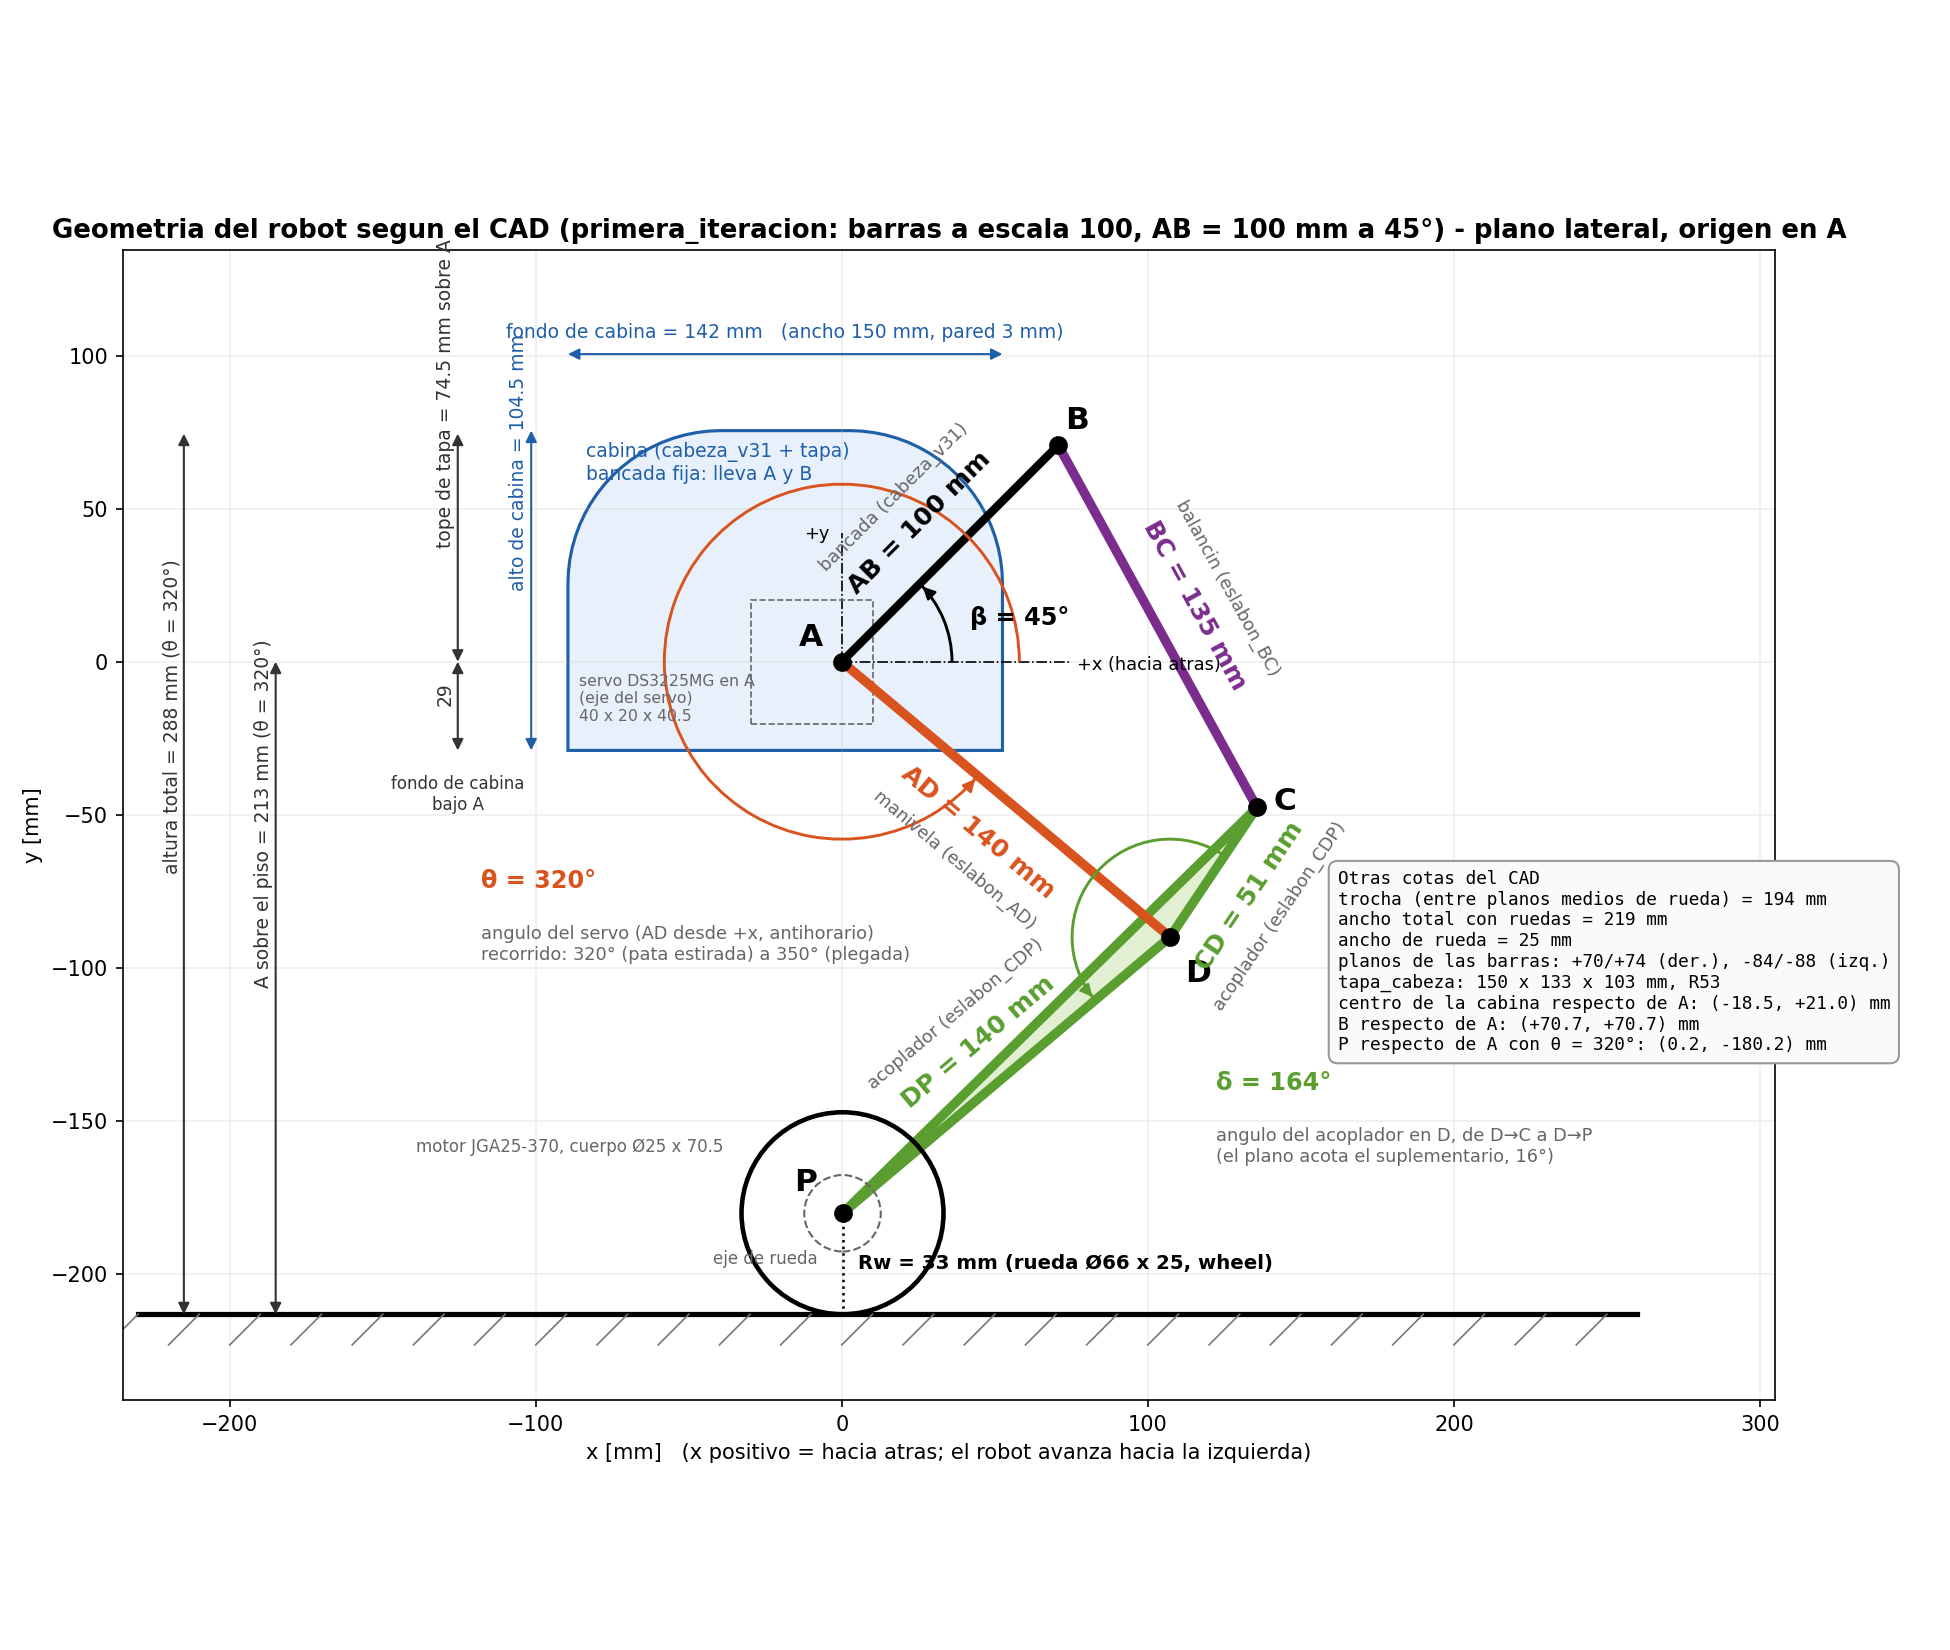
\includegraphics[width=0.93\textwidth]{geometria_robot.png}
\captionof{figure}{El robot con la pata en su postura media. Los nombres $A$, $B$, $C$, $D$
y $P$ se usan en todo el documento.}
\end{center}

\section{Las masas}

\begin{medido}
El 21/10/2026 se pesaron por primera vez las piezas. Las tres barras, una por una, y el robot
entero \emph{sin ruedas ni motores de rueda}: 670 g. Restando las seis barras, la caja queda
en 542 g. El 22/10 llegaron las ruedas y los motores de rueda y también se pesaron: con eso
están \textbf{todas} las masas del robot medidas.
\end{medido}

\begin{center}
\begin{tabular}{@{}llrr@{}}
\toprule
\textbf{Pieza} & \textbf{Estado} & \textbf{Modelo viejo} & \textbf{Hoy} \\
\midrule
Manivela $AD$ (cada una) & \textcolor{verdep}{medida} & 23{,}2 g & \textbf{30 g} \\
Balancín $BC$ (cada uno) & \textcolor{verdep}{medida} & 5{,}6 g & \textbf{23 g} \\
Acoplador $CDP$ (cada uno) & \textcolor{verdep}{medida} & 15{,}6 g & \textbf{11 g} \\
Caja (todo lo que no es pata) & \textcolor{verdep}{medida por diferencia} & 667 g & \textbf{542 g} \\
Rueda (cada una) & \textcolor{verdep}{medida} & 30 g & \textbf{50 g} \\
Motor de rueda (cada uno) & \textcolor{verdep}{medida} & 95 g & \textbf{96 g} \\
\midrule
\textbf{Robot completo} & & 1006 g & \textbf{962 g} \\
\bottomrule
\end{tabular}
\end{center}

Tres sorpresas, y las tres enseñan algo:

\begin{itemize}[leftmargin=1.5em]
\item El \textbf{balancín pesa cuatro veces} lo que decía el modelo. Era la pieza más chica y
      la que peor se estimó. Moraleja: las estimaciones por volumen no son confiables cuando
      la pieza es pequeña, porque el relleno de la impresión 3D pesa relativamente más.
\item La \textbf{caja pesa un 19\% menos}. Acá la moraleja es al revés: el modelo era pesimista,
      y al corregirlo \emph{mejoraron} los márgenes. El par que pide el servo bajó de 9{,}06 a
      \textbf{7{,}98 kg$\cdot$cm}, y su margen subió de 4{,}4 a \textbf{5{,}0}.
\item La \textbf{rueda pesa un 67\% más} (50 g contra 30). Pero acá hay una buena noticia
      escondida: la rueda y el motor están \emph{en el eje}, así que no cambian nada del péndulo
      ---ni el brazo, ni la inercia del cuerpo, ni el par de la gravedad---. Lo único que
      mueven es la masa que hay que acelerar para avanzar, y el peso sobre el piso, que
      \emph{mejora} el agarre.
\end{itemize}

\section{Los componentes}

\begin{center}
\small
\begin{tabular}{@{}llp{7.4cm}@{}}
\toprule
\textbf{Qué} & \textbf{Cuántos} & \textbf{Cuál} \\
\midrule
Motor de rueda & 2 & GA25-370, 12 V, 300 rpm en vacío, reducción 1:20, con encoder de
cuadratura \\
Driver de motor & 2 & DRV8871, puente H con PWM \\
Servo de pata & 2 & DSSERVO DS3240 MG, etiqueta 40 kg$\cdot$cm \\
Controlador & 1 & ESP32-S3 DevKitC-1 N16R8 \\
IMU & 1 & MPU-6050 \\
Batería & 1 & tres celdas, 11{,}1 V nominales \\
\bottomrule
\end{tabular}
\end{center}

% ===========================================================================
\chapter{La pata: cinemática}\label{cap:cin}
% ===========================================================================

\begin{idea}
El cuatro barras tiene un solo grado de libertad. Dado $\theta$, la posición de cada punto
sale de resolver el cierre del mecanismo con dos triángulos. Lo que importa del resultado es
cómo sube el eje de la rueda $P$ cuando el servo gira.
\end{idea}

\section{El cierre del mecanismo}

El lazo $A\!\to\!B\!\to\!C\!\to\!D\!\to\!A$ tiene que cerrar. La forma más cómoda de
resolverlo es cortar por la diagonal $BD$, que convierte el cuadrilátero en dos triángulos:

\begin{equation}
BD(\theta) = \sqrt{AB^2 + AD^2 - 2\,AB\,AD\cos(\theta + \alpha_{AB})},
\end{equation}

con $\alpha_{AB} = 45^\circ$ la inclinación de la bancada. Después, por el teorema del coseno
en cada triángulo, salen los cuatro ángulos auxiliares:

\begin{align}
\cos\beta_1 &= \frac{AB^2 + BD^2 - AD^2}{2\,AB\,BD}, &
\cos\beta_2 &= \frac{BC^2 + BD^2 - CD^2}{2\,BC\,BD}, \\
\cos\alpha_1 &= \frac{AD^2 + BD^2 - AB^2}{2\,AD\,BD}, &
\cos\alpha_2 &= \frac{CD^2 + BD^2 - BC^2}{2\,CD\,BD},
\end{align}

y de ahí el ángulo del acoplador:
\begin{equation}
\psi = \pi - \theta - \alpha_1 - \alpha_2 .
\end{equation}

Con $\psi$ ya está todo: $C = D + CD\,(\cos\psi,\ \sin\psi)$ y
$P = D + DP\,(\cos(\psi+\delta),\ \sin(\psi+\delta))$.

\begin{ojo}
El teorema del coseno tiene dos soluciones, una por cada rama de armado del mecanismo. El
modelo usa siempre la rama $+1$, que es la del CAD. Si en algún cálculo apareciera la otra,
la pata se dibujaría dada vuelta. Por eso el código verifica el cierre y aborta si el ángulo
pedido no es alcanzable.
\end{ojo}

\section{Lo que importa del resultado}

\begin{center}
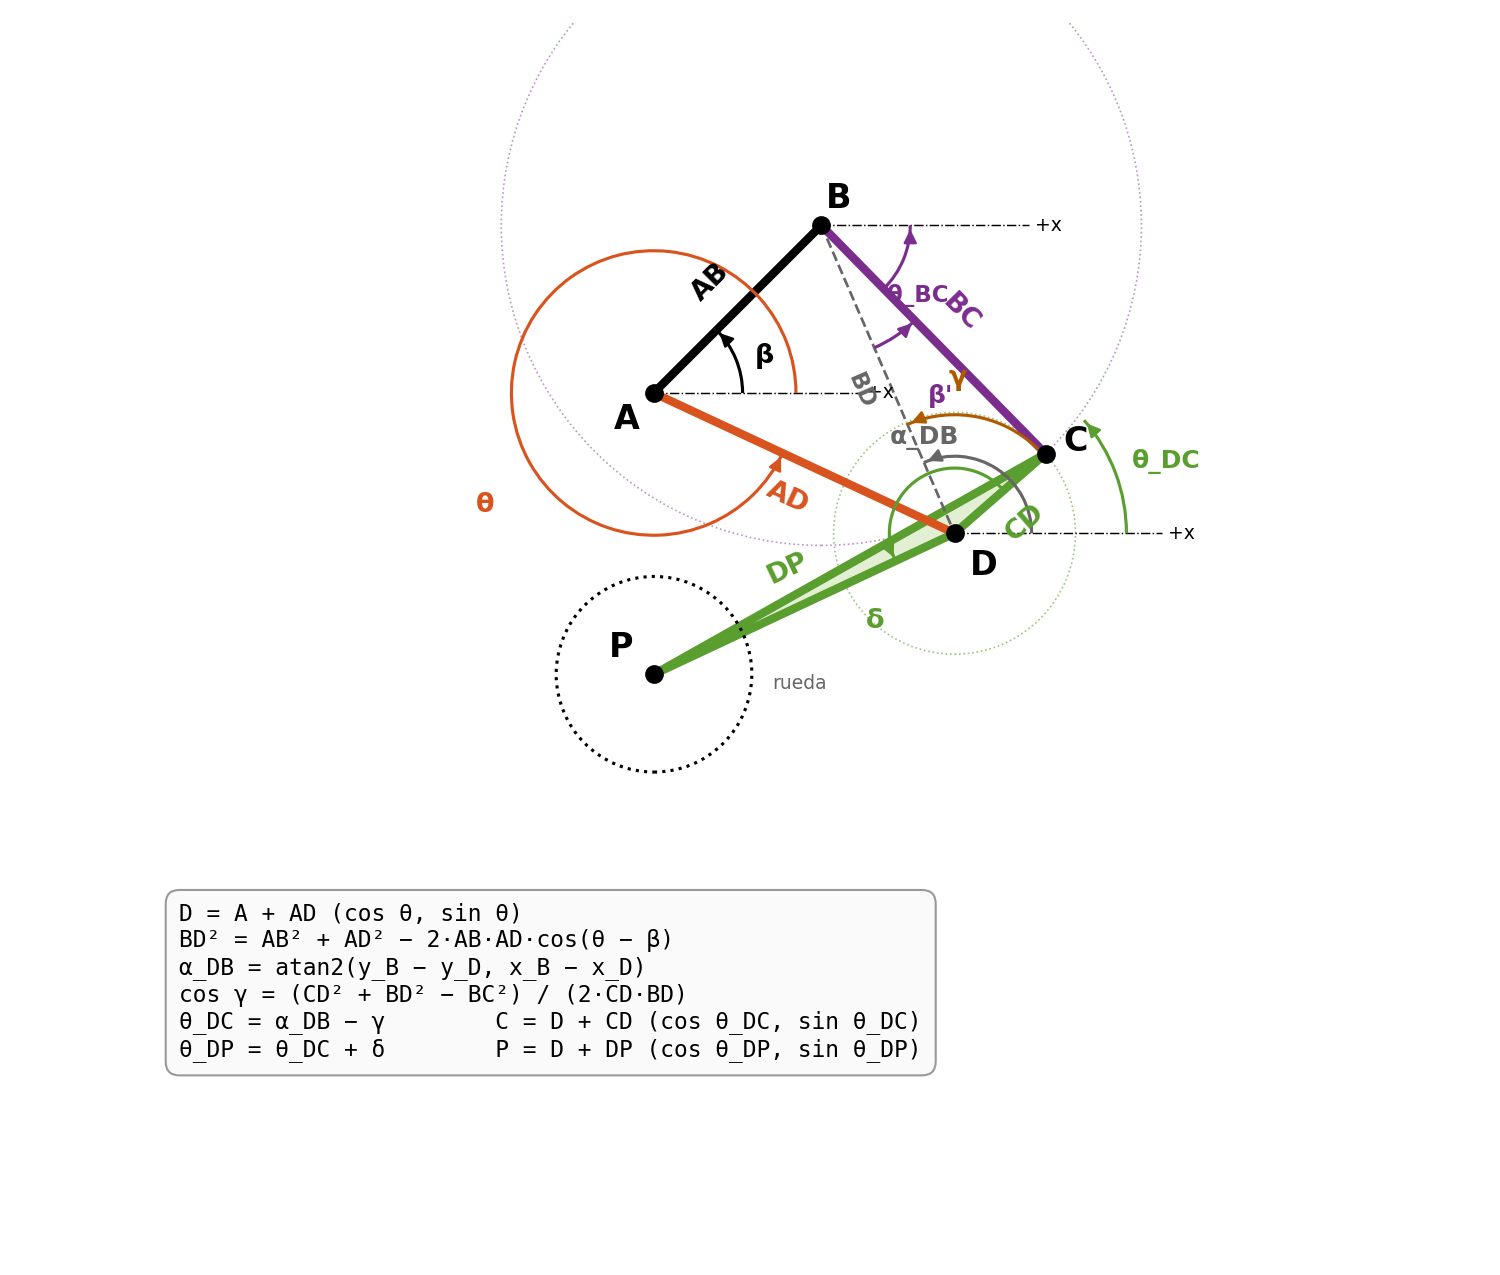
\includegraphics[width=0.95\textwidth]{fig_cinematica_directa.png}
\captionof{figure}{La pata en varias posturas y la trayectoria del eje de la rueda.}
\end{center}

De toda la cinemática, lo que entra en la dinámica es una sola función: $y_P(\theta)$, la
altura del eje de la rueda, y sobre todo su derivada $y_P'(\theta)$. Esa derivada es la
\emph{ventaja mecánica} del mecanismo: cuántos milímetros sube la rueda por cada radián que
gira el servo. Es la que decide cuánto par hace falta.

El desarrollo completo, con todas las derivadas y la verificación numérica, está en el
apéndice \ref{ap:cin}.

% ===========================================================================
\chapter{La pata: dinámica}\label{cap:din}
% ===========================================================================

\begin{idea}
Como el mecanismo tiene un solo grado de libertad, toda su dinámica se reduce a una ecuación
escalar en $\theta$. Lo único que cambia entre el banco de pruebas, el robot parado y el robot
en el aire es \emph{qué está quieto}, y eso entra como un solo vector.
\end{idea}

\section{Una ecuación, tres situaciones}

Por Lagrange, con $\theta$ como coordenada generalizada:

\begin{equation}\label{eq:pata}
I_{eq}(\theta)\,\ddot\theta
\;+\;\tfrac12\,I_{eq}'(\theta)\,\dot\theta^{\,2}
\;+\;V'(\theta)
\;=\;\tau \;-\; b\,\dot\theta \;+\; N\,y_P'(\theta).
\end{equation}

El término $\tfrac12 I_{eq}'\dot\theta^2$ es el de Coriolis y centrífugo: aparece porque la
inercia equivalente \emph{cambia} con la postura. $V'(\theta)$ es el par que hace la gravedad.
$N$ es la normal del piso, que sólo actúa cuando la rueda apoya.

Los tres casos difieren en un solo vector, $u(\theta)$, que es la velocidad de la cabina por
unidad de $\dot\theta$:

\begin{center}
\begin{tabular}{@{}llp{7.0cm}@{}}
\toprule
\textbf{Caso} & $u(\theta)$ & \textbf{Qué representa} \\
\midrule
\texttt{banco} & $0$ & la cabina está amurada y sube y baja la rueda \\
\texttt{parado} & $-c_P$ & la rueda apoya y sube y baja la cabina: \textbf{el robot real de pie} \\
\texttt{aire} & $-2S/m$ & nada está quieto; el centro de masa no se mueve \\
\bottomrule
\end{tabular}
\end{center}

\begin{center}
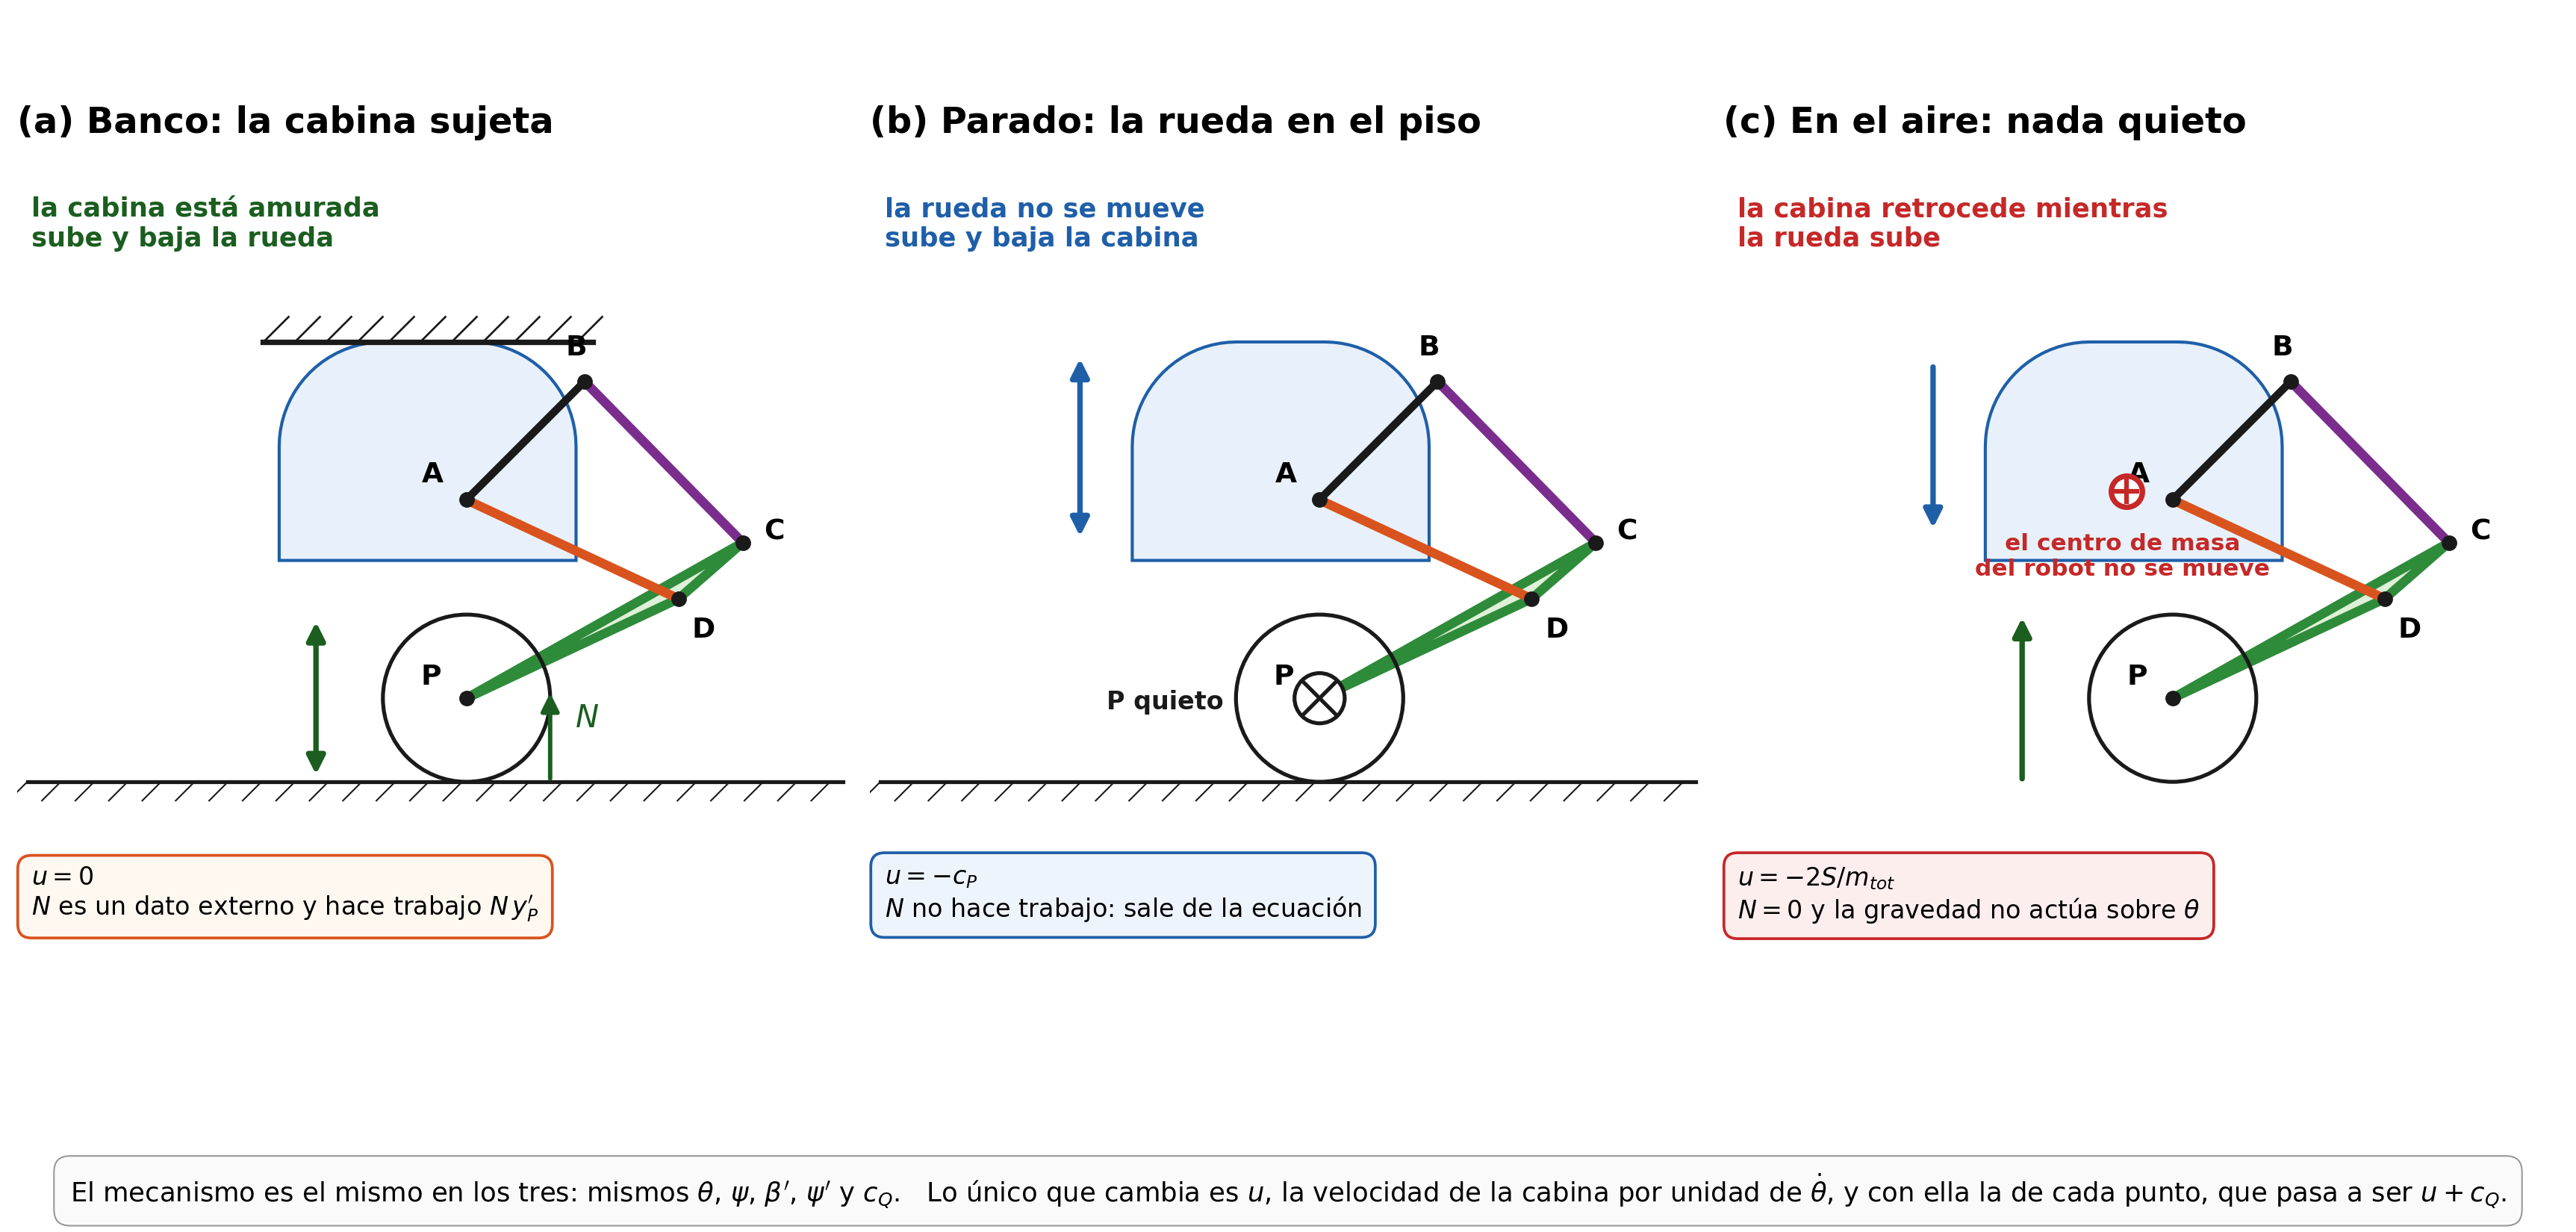
\includegraphics[width=0.95\textwidth]{fig_casos.png}
\captionof{figure}{Los tres casos con el mismo mecanismo. Lo que cambia es qué está quieto.}
\end{center}

\section{Qué sale de ahí}

\begin{center}
\begin{tabular}{@{}lrrr@{}}
\toprule
& $\theta = 10^\circ$ & $\theta = 25^\circ$ & $\theta = 40^\circ$ \\
\midrule
$I_{eq}$ caso \texttt{banco} [g$\cdot$m$^2$] & 9{,}56 & 6{,}23 & 5{,}29 \\
$I_{eq}$ caso \texttt{parado} [g$\cdot$m$^2$] & 19{,}42 & 12{,}30 & 10{,}47 \\
Par estático del servo [kg$\cdot$cm] & \textbf{7{,}98} & 6{,}33 & 5{,}78 \\
\bottomrule
\end{tabular}
\end{center}

Dos lecturas:

\begin{itemize}[leftmargin=1.5em]
\item Parado, el servo ve una inercia \textbf{2{,}0 veces} mayor que en el banco. Tiene
      sentido: en el banco mueve la rueda, parado mueve el robot entero.
\item El peor caso es la pata \textbf{plegada}, con 7{,}98 kg$\cdot$cm por servo. Con el
      DS3240 de 40 kg$\cdot$cm el margen es \textbf{5{,}0}. El servo está holgado.
\end{itemize}

\section{La verificación que vale la pena}

La ecuación \eqref{eq:pata} se obtuvo por Lagrange, que es un método de energías y no muestra
las fuerzas internas. Para comprobarla se resolvió el mismo problema por el camino opuesto:
diagramas de cuerpo libre de las tres barras, nueve ecuaciones de equilibrio con nueve
incógnitas: $A_x$, $A_y$, $\tau$, $B_x$, $B_y$, $C_x$, $C_y$, $D_x$ y $D_y$.

\begin{center}
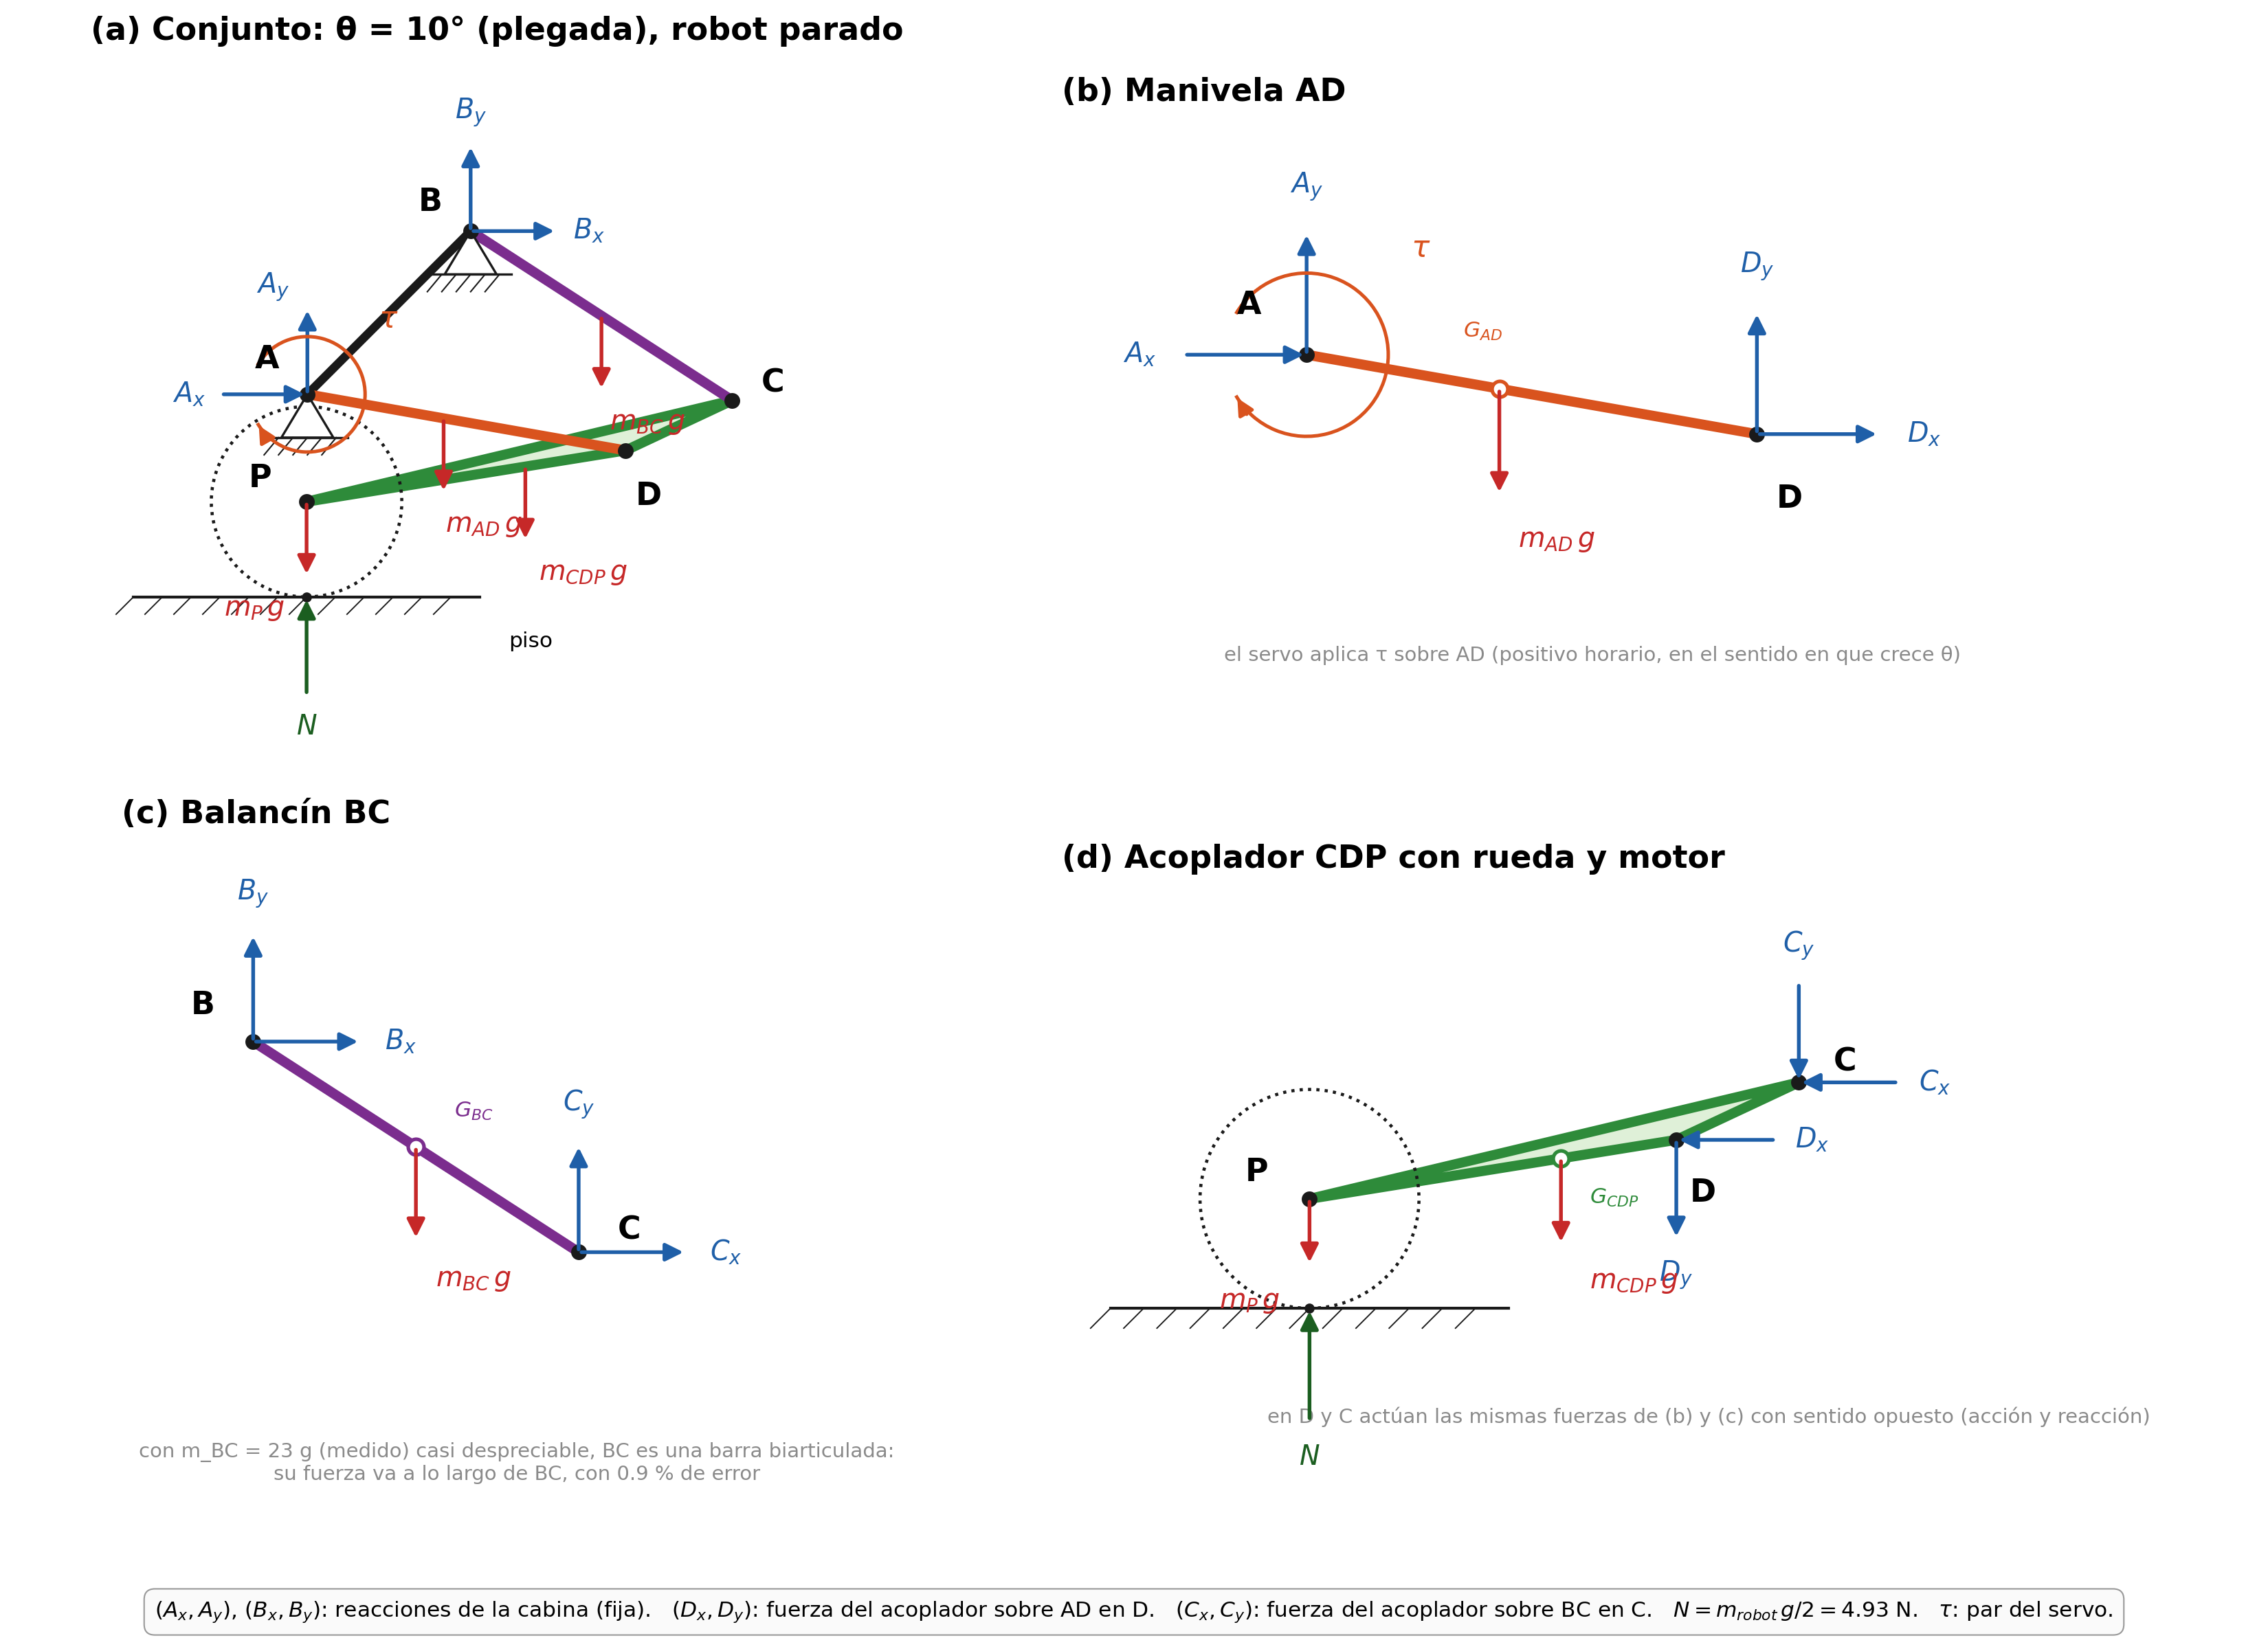
\includegraphics[width=0.95\textwidth]{dcl_pata.png}
\captionof{figure}{Los tres cuerpos de la pata con todas sus fuerzas. Resolver este sistema
da el mismo par que Lagrange hasta el redondeo de máquina.}
\end{center}

Los dos caminos dan el mismo par con una diferencia de $8\times10^{-16}$ N$\cdot$m, que es
precisión de máquina. Son métodos independientes, así que coincidir es evidencia fuerte de
que los dos están bien. El desarrollo está en el apéndice \ref{ap:dcl}.

\section{Aterrizar de un escalón}

\begin{idea}
Cuando el robot cae de un escalón hay \textbf{dos golpes distintos}, y conviene no
confundirlos, porque los absorben cosas distintas.
\end{idea}

\begin{center}
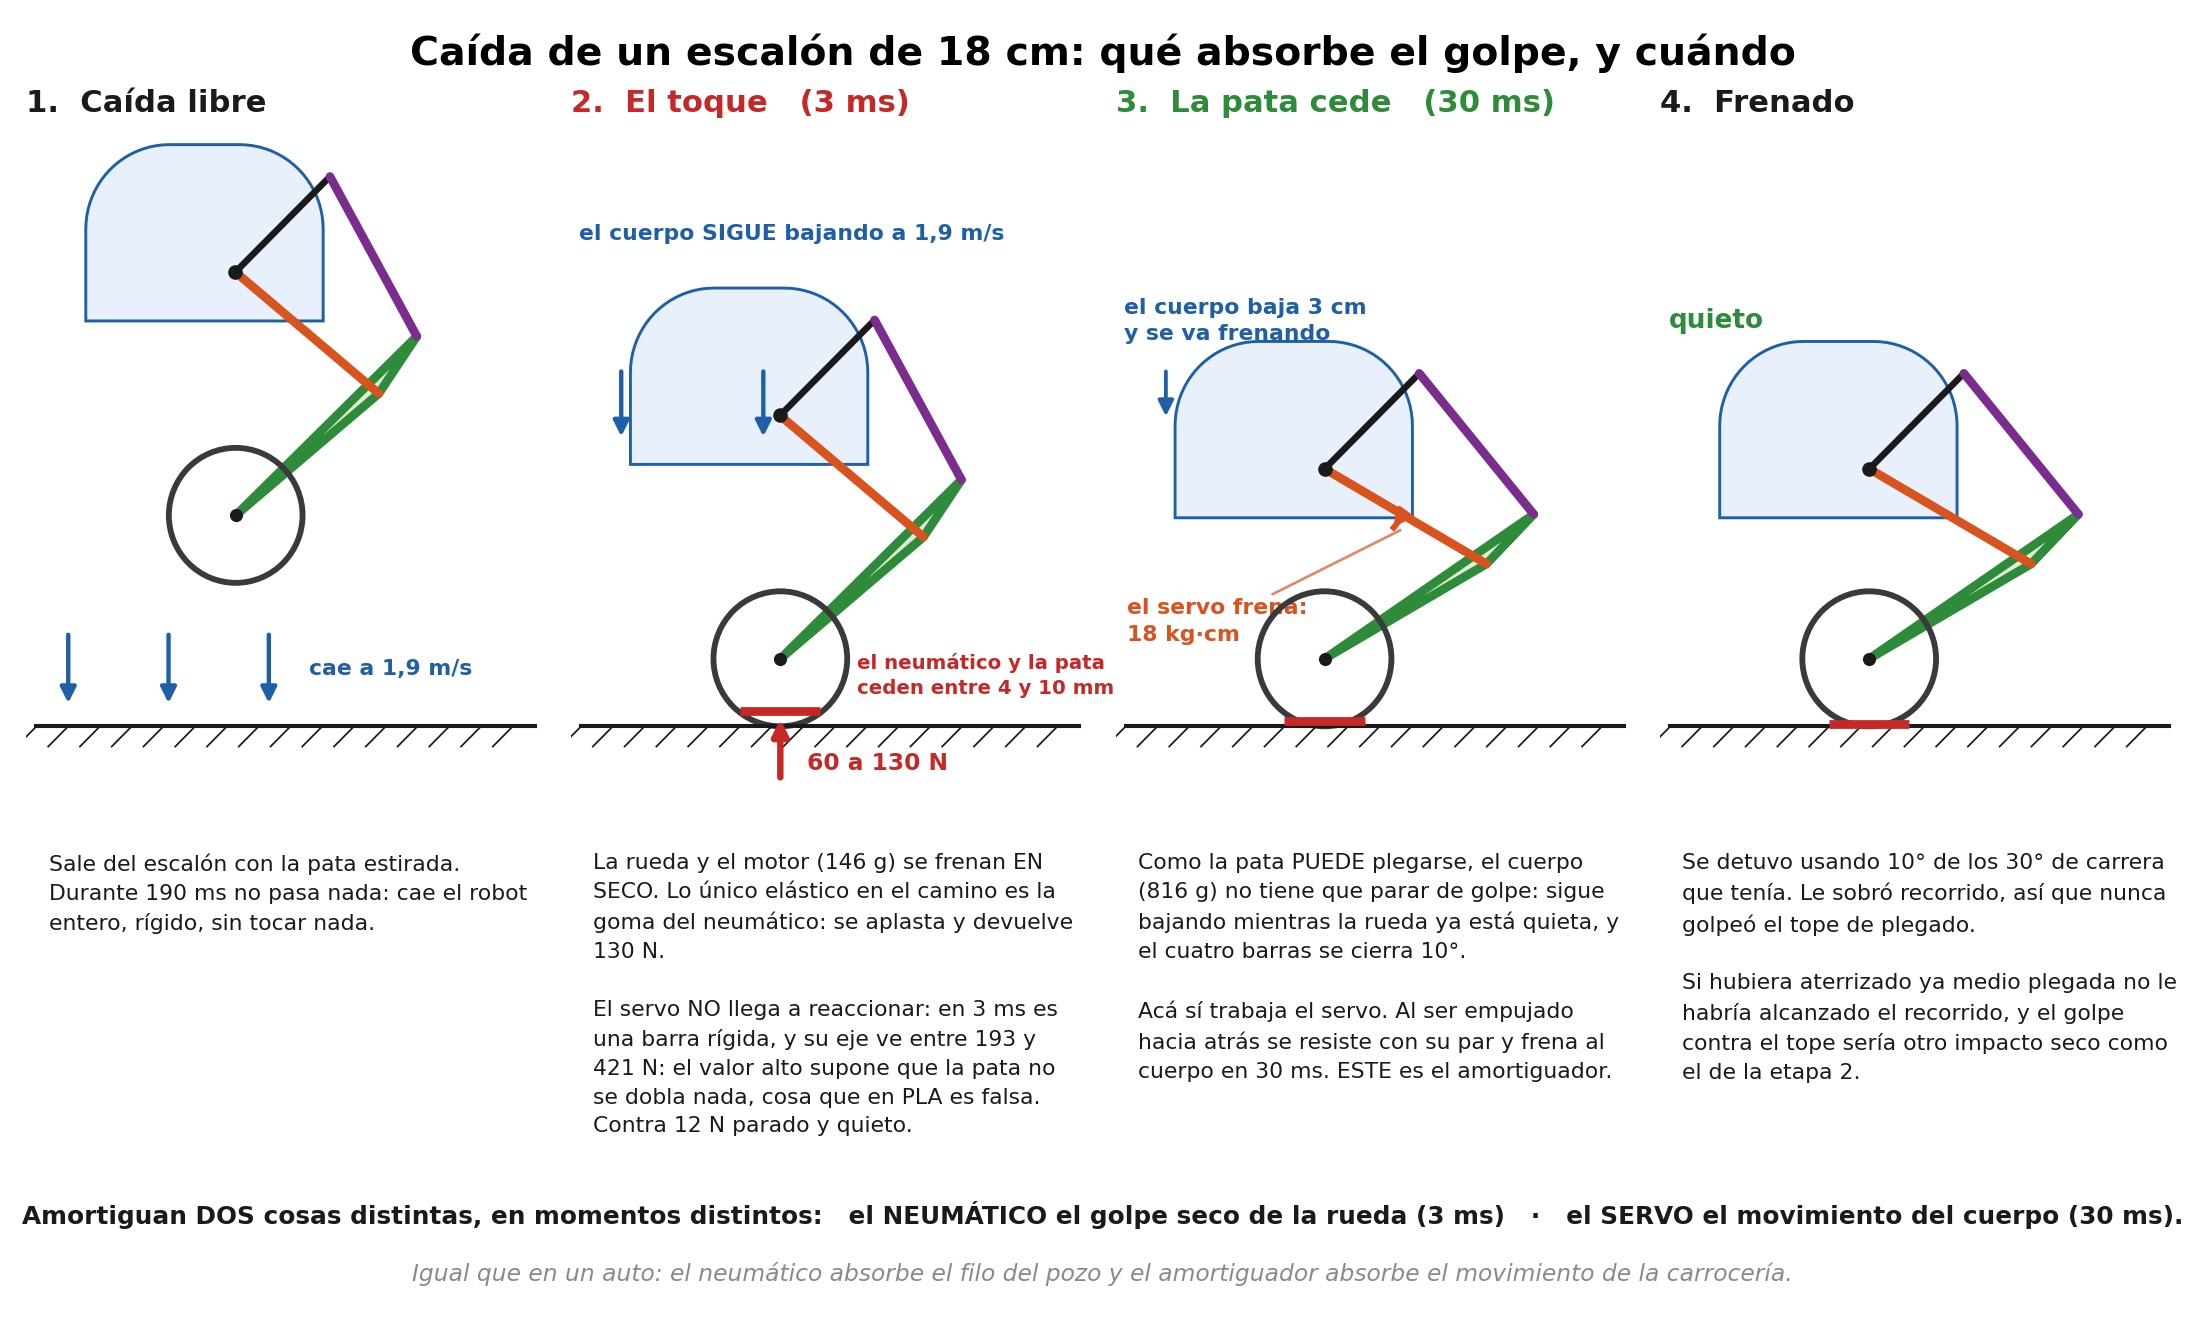
\includegraphics[width=\textwidth]{fig_aterrizaje.png}
\captionof{figure}{La secuencia del aterrizaje desde un escalón de 18 cm.}
\end{center}

\begin{center}
\begin{tabular}{@{}lll@{}}
\toprule
& \textbf{Fase A: el toque} & \textbf{Fase B: el frenado} \\
\midrule
Dura & $\sim$3 ms & 11 a 33 ms \\
Qué se frena & la rueda y el motor, 146 g, en seco & el resto del robot, 816 g \\
Quién lo absorbe & \textbf{sólo el neumático} & el servo plegando la pata \\
El servo & no reacciona: es una barra rígida & trabaja, 8 a 18 kg$\cdot$cm \\
Fuerza en el eje del servo & 64 N (2 cm) a 193 N (18 cm)$^*$ & 94 N \\
\bottomrule
\end{tabular}
\end{center}
{\small $^*$ Contando la pata de PLA como un resorte de 8 kN/m en serie con el neumático. Si se la
supone rígida ---que es lo que hacía el primer cálculo--- dan 140 y 421 N, pero eso es una cota
superior: la manivela impresa es tan blanda como el neumático, y en serie manda la más blanda.
Se mide con el ensayo M-7.}


La fase B está cubierta: el servo absorbe 0{,}9 J usando 10 de los 30 grados de carrera.
La que preocupa es la fase A.

\begin{ojo}
En 3 ms el servo no llega a reaccionar: mantiene posición y transmite todo. El pico sale de
$F = \sqrt{2Ek}$, con $E$ la energía de la masa \emph{no suspendida} (rueda más motor) y $k$
la rigidez del neumático. Un neumático tres veces más blando baja el pico un 42\%; uno tres
veces más duro lo sube un 73\%.

La recomendación de diseño que sale de acá: que el pasador $A$ tenga \textbf{rodamiento
propio} tomando la carga radial, y que el servo entregue sólo par. Casi 200 N sobre el estriado de
un servo le arranca los dientes.
\end{ojo}

% ===========================================================================
\chapter{El péndulo invertido: la planta que se controla}\label{cap:pend}
% ===========================================================================

\begin{idea}
Con las patas congeladas, el robot es un péndulo invertido sobre ruedas: dos grados de
libertad, $x$ (avance) y $\varphi$ (inclinación), y una sola entrada, el par de los motores.
Un actuador para dos coordenadas: por eso el problema no es trivial.
\end{idea}

\section{Las coordenadas}

\begin{center}
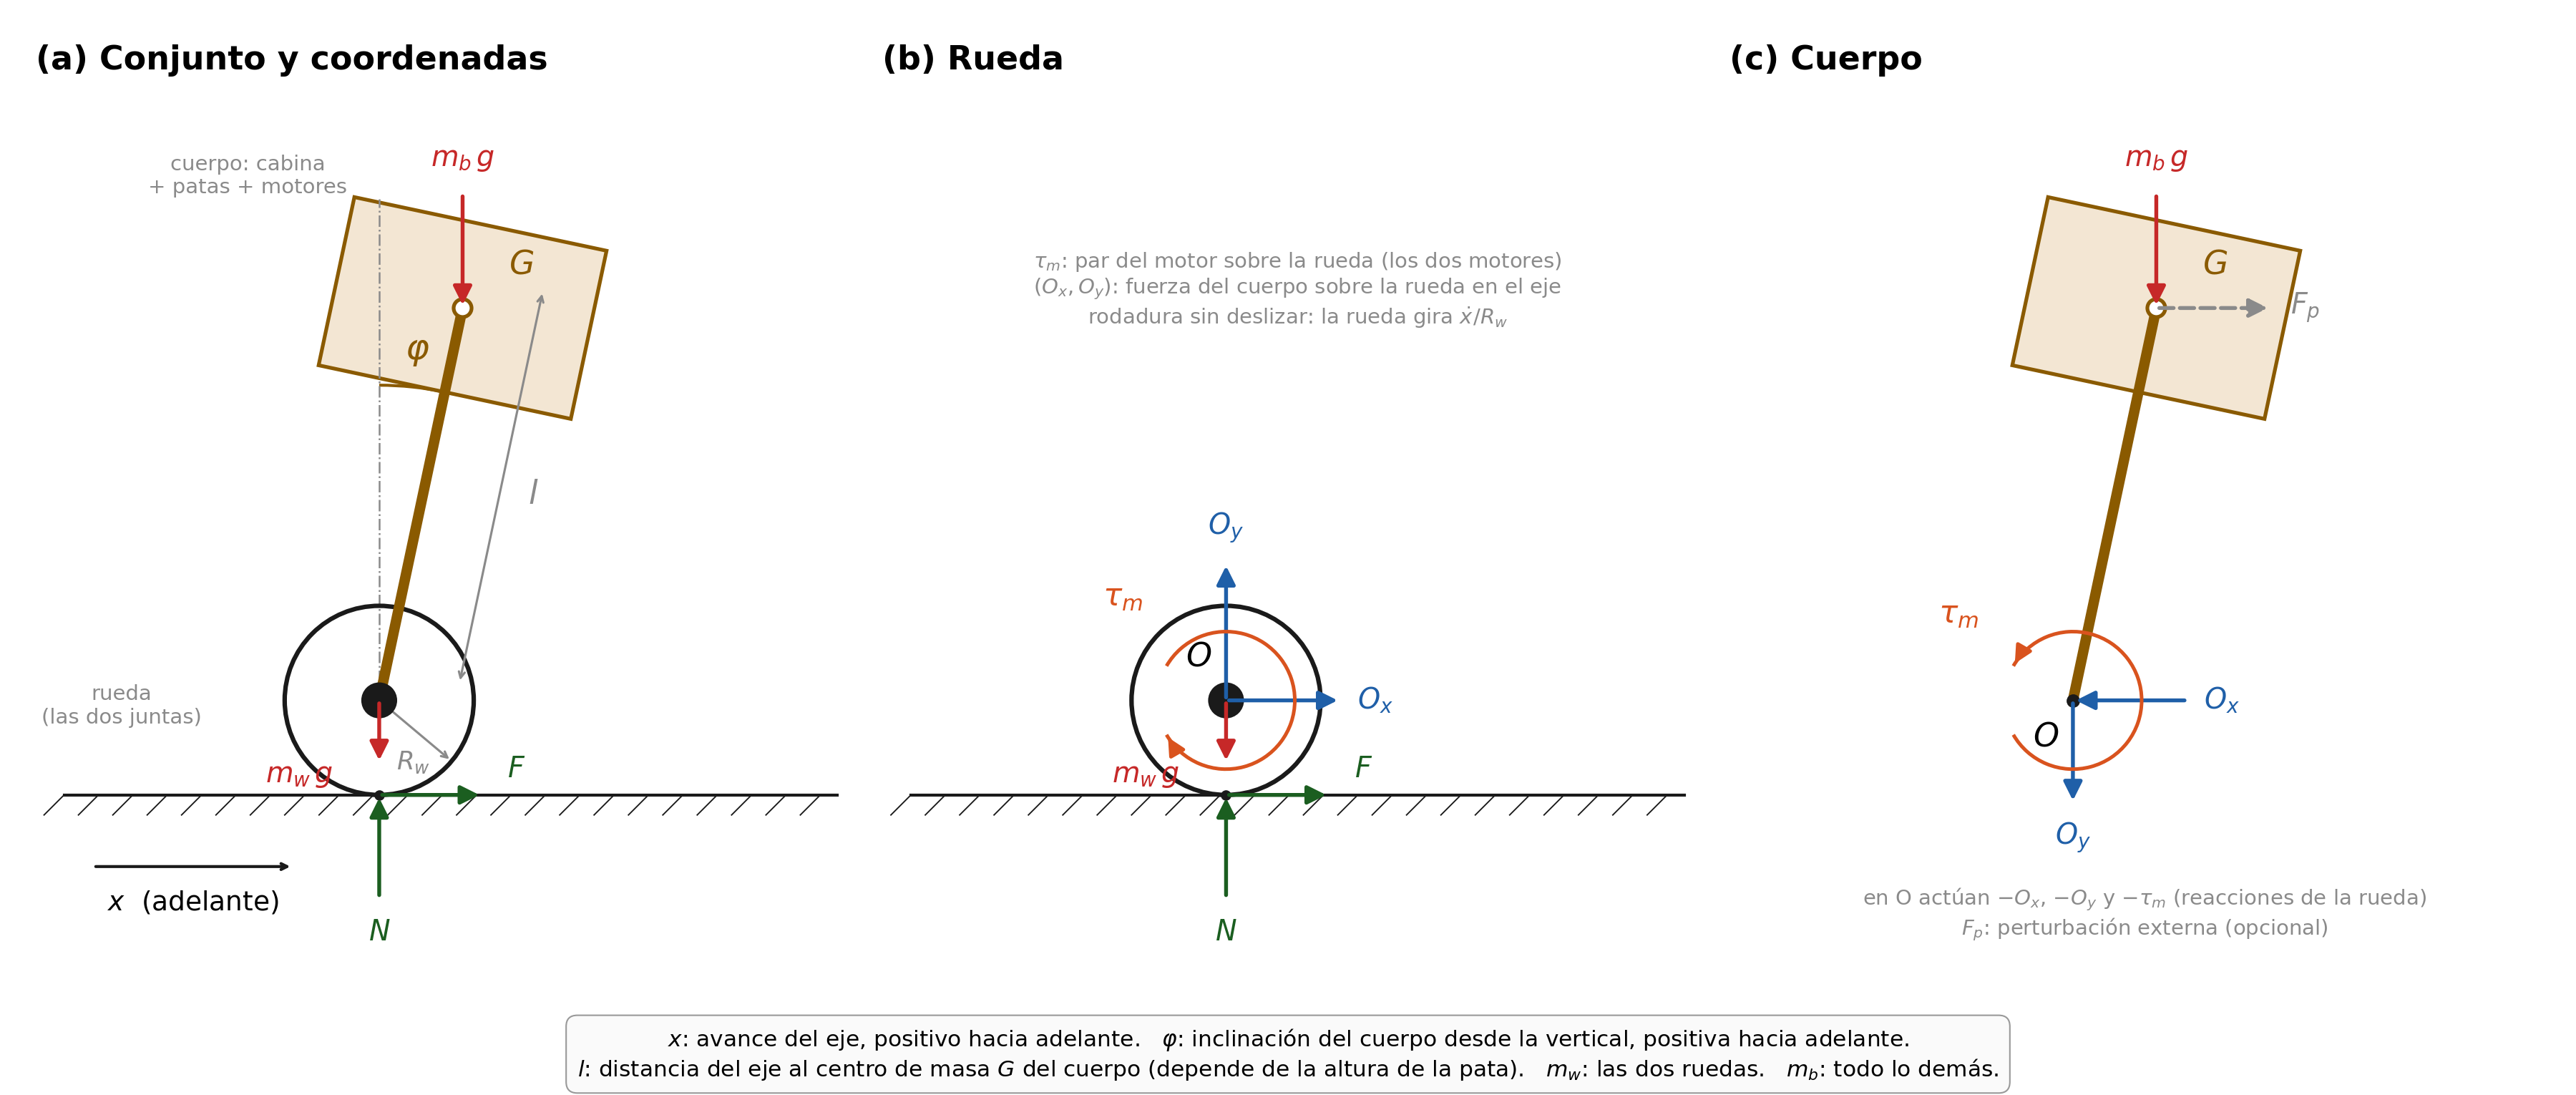
\includegraphics[width=0.78\textwidth]{dcl_segway.png}
\captionof{figure}{Los dos cuerpos: la rueda (las dos juntas) y el cuerpo (cabina, patas y
motores). $x$ es el avance del eje, positivo hacia adelante, y $\varphi$ la inclinación del
cuerpo desde la vertical, positiva hacia adelante.}
\end{center}

La rueda rueda sin deslizar, así que gira $\dot x / R_w$. Los motores aplican $\tau$ sobre la
rueda y, por reacción, $-\tau$ sobre el cuerpo. Ese par de reacción es \emph{la única forma}
que tiene el robot de inclinarse a voluntad.

\begin{ojo}
$\varphi$ \textbf{no} es el ángulo del chasis. Se mide desde la dirección del centro de masa,
que no coincide con la vertical del chasis: hay entre medio un ángulo $\delta_G$ que vale
$-3{,}58^\circ$ en la postura media, porque el centro de masa cae 5 mm por \emph{detrás} del
eje. La IMU mide el chasis, así que el firmware tiene que sumarle $\delta_G$. El capítulo
\ref{cap:patasmov} muestra qué pasa si no lo hace.
\end{ojo}

\section{Las ecuaciones: de dónde salen}

\begin{idea}
Se escribe la energía del robot en función de dos coordenadas, se le aplica Lagrange y sale
todo. Lo único que hay que tener cuidado es con los signos y con el rotor del motor, que
aporta una inercia que no se ve.
\end{idea}

\subsection{Qué se modela y qué se deja afuera}

\begin{center}
\small
\begin{tabular}{@{}p{7.2cm}p{7.2cm}@{}}
\toprule
\textbf{Está en el modelo} & \textbf{No está} \\
\midrule
las dos ruedas, con su masa y su inercia & el giro: las dos ruedas van juntas \\
el cuerpo entero (cabina, patas y motores) como \emph{un solo} sólido rígido & el movimiento de las patas: están congeladas \\
el rotor de los motores, con su inercia reflejada & la elasticidad de las barras \\
la reacción del par sobre el cuerpo & el deslizamiento: la rueda no patina \\
rozamiento viscoso en el eje y en el pivote & el rozamiento seco \\
\bottomrule
\end{tabular}
\end{center}

Que el cuerpo sea \emph{un} sólido rígido es la hipótesis más fuerte, y es legítima
precisamente porque las patas están quietas: con las patas bloqueadas, cabina, barras y
motores se mueven todos juntos, así que se los puede reemplazar por un único cuerpo con la
masa total, su centro de masa y su inercia. El capítulo \ref{cap:patasmov} revisa qué pasa
cuando se las suelta.

\subsection{Las coordenadas}

Dos grados de libertad, y los dos con el signo que uno espera:

\begin{center}
\begin{tabular}{@{}llp{9.4cm}@{}}
\toprule
$x$ & [m] & cuánto avanzó el \textbf{eje de las ruedas}. Positivo \textbf{hacia adelante},
que es el lado hacia el que no sobresale la rodilla de la pata \\
$\varphi$ & [rad] & inclinación del cuerpo desde la vertical. Positiva cuando el centro de
masa se va \textbf{hacia adelante} del eje, o sea cuando el robot se tira para adelante \\
$\tau$ & [N$\cdot$m] & par de los motores sobre las ruedas. Positivo cuando \textbf{empuja
hacia adelante} \\
\bottomrule
\end{tabular}
\end{center}

\begin{idea}
Con este convenio todo se lee como uno espera: \textbf{el robot se inclina hacia adelante
(}$\varphi > 0$\textbf{) para ir hacia adelante}, y un par positivo lo empuja hacia adelante.
Es el mismo convenio del apéndice \ref{ap:dcl}, el informe de diagramas de cuerpo libre, así
que los dos documentos se pueden leer juntos sin traducir nada.

Hasta el 22/10/2026 el modelo usaba el convenio opuesto para $\varphi$ y $\tau$. Era
igual de válido, pero obligaba a decir que ``para avanzar, $\varphi$ se hace negativo'', que
es exactamente la clase de frase que confunde en una defensa. Se dio vuelta a propósito.
\end{idea}

La rodadura sin deslizar ata el giro de la rueda al avance. Llamando $\theta_w$ al ángulo
girado por la rueda, positivo en el sentido que hace avanzar al robot:

\begin{equation}\label{eq:rodadura}
\theta_w = \frac{x}{R_w}
\qquad\Longrightarrow\qquad
\dot\theta_w = \frac{\dot x}{R_w}.
\end{equation}

\subsection{Dónde está cada cosa}

Poniendo el origen en el punto donde el eje arranca, y con el piso en $y = 0$:

\begin{align}
\text{eje de las ruedas:}&\qquad (x,\ R_w) \\
\text{centro de masa del cuerpo:}&\qquad
\begin{cases}
x_G = x + \ell\,\sin\varphi \\
y_G = R_w + \ell\,\cos\varphi
\end{cases}
\end{align}

con $\ell$ la distancia del eje al centro de masa. Derivando:

\begin{equation}
\dot x_G = \dot x + \ell\cos\varphi\,\dot\varphi,
\qquad
\dot y_G = -\ell\sin\varphi\,\dot\varphi .
\end{equation}

\subsection{La energía cinética, término por término}

\textbf{Las ruedas} (las dos juntas: masa $m_w$, inercia $J_w$) se trasladan con el eje y giran
según \eqref{eq:rodadura}:

\begin{equation}
T_w = \tfrac12\,m_w\,\dot x^{\,2} \;+\; \tfrac12\,J_w\left(\frac{\dot x}{R_w}\right)^{\!2}
    = \tfrac12\left(m_w + \frac{J_w}{R_w^2}\right)\dot x^{\,2}.
\end{equation}

Acá ya aparece algo que vale la pena notar: la inercia de la rueda se \emph{suma a la masa},
dividida por el radio al cuadrado. Una rueda pesada cuesta más de acelerar dos veces: una por
su masa y otra por su inercia.

\textbf{El cuerpo} (masa $m_b$, inercia $J_b$ respecto de \emph{su propio} centro de masa):

\begin{align}
T_b &= \tfrac12\,m_b\left(\dot x_G^{\,2} + \dot y_G^{\,2}\right) + \tfrac12\,J_b\,\dot\varphi^{\,2}\\
    &= \tfrac12\,m_b\Bigl[\bigl(\dot x + \ell\cos\varphi\,\dot\varphi\bigr)^2
       + \ell^2\sin^2\!\varphi\,\dot\varphi^{\,2}\Bigr] + \tfrac12\,J_b\,\dot\varphi^{\,2}\\
    &= \tfrac12\,m_b\,\dot x^{\,2}
       \;+\; m_b\,\ell\cos\varphi\;\dot x\,\dot\varphi
       \;+\; \tfrac12\bigl(J_b + m_b\ell^2\bigr)\dot\varphi^{\,2}.
\end{align}

En el último paso se usó $\cos^2 + \sin^2 = 1$, que es lo que hace desaparecer la dependencia
con $\varphi$ del último término. Notar que $J_b + m_b\ell^2$ es, por Steiner, la inercia del
cuerpo respecto del \textbf{eje de la rueda}, no respecto de su centro de masa.

\textbf{Los rotores} son el término que casi siempre se olvida, y acá pesa mucho. El rotor de
cada motor gira respecto del \emph{cuerpo}, que a su vez gira. Con reducción $n$:

\begin{equation}\label{eq:rotor}
\dot\alpha_m = n\,\frac{\dot x}{R_w} \;+\; (1-n)\,\dot\varphi .
\end{equation}

El primer término es el giro de la rueda multiplicado por la reducción; el segundo es que, si
el cuerpo gira, el estator gira con él. Con $n_{mot}$ motores de inercia de rotor $J_r$:

\begin{equation}
T_r = \tfrac12\,n_{mot}J_r\,\dot\alpha_m^{\,2}
= \tfrac12\,\frac{n_{mot}J_r n^2}{R_w^2}\,\dot x^{\,2}
\;+\; \underbrace{\frac{n_{mot}J_r\,n(1-n)}{R_w}}_{\textstyle e}\,\dot x\,\dot\varphi
\;+\; \tfrac12\,n_{mot}J_r(1-n)^2\,\dot\varphi^{\,2}.
\end{equation}

\begin{ojo}
Mirá el término del medio: es un acoplamiento entre $\dot x$ y $\dot\varphi$, igual que el del
cuerpo, \textbf{pero no lleva $\cos\varphi$}. La ecuación \eqref{eq:rotor} es lineal con
coeficientes fijos: no depende de la postura. Por eso el acoplamiento total queda
$h\cos\varphi + e$, con dos partes de naturaleza distinta, y el $e$ \emph{no} se puede meter
adentro de $h$.

Y además $e$ es \textbf{negativo}, porque $n > 1$ hace que $n(1-n) < 0$: el rotor acopla al
revés que el cuerpo. Con $e = 0$ se recupera el modelo clásico de péndulo invertido sobre
ruedas que está en los libros, que no tiene rotor.
\end{ojo}

\textbf{Sumando todo}, la energía cinética queda, ordenada:

\begin{equation}\label{eq:T}
T = \tfrac12\,a\,\dot x^{\,2}
\;+\; \bigl(h\cos\varphi + e\bigr)\,\dot x\,\dot\varphi
\;+\; \tfrac12\,j\,\dot\varphi^{\,2}
\;=\; \tfrac12\,\dot q^{\,\mathsf{T}} M(\varphi)\,\dot q,
\end{equation}

que es \emph{exactamente} la forma $\tfrac12 \dot q^{\mathsf T} M \dot q$ con la matriz de masa
de la ecuación \eqref{eq:planta}. Y ahora se ve de dónde sale cada coeficiente:

\begin{center}
\small
\begin{tabular}{@{}llr@{}}
\toprule
\textbf{Coef.} & \textbf{Fórmula} & \textbf{Valor} \\
\midrule
$a$ & $\underbrace{m_b + m_w}_{0{,}962} + \underbrace{J_w/R_w^2}_{0{,}050} + \underbrace{n_{mot}J_r n^2/R_w^2}_{0{,}300}$ & 1{,}3119 kg \\[10pt]
$h$ & $m_b\,\ell = 0{,}8619 \times 0{,}0815$ & 0{,}07024 kg$\cdot$m \\[4pt]
$j$ & $\underbrace{J_b}_{0{,}003860} + \underbrace{m_b\ell^2}_{0{,}005725} + \underbrace{n_{mot}J_r(1-n)^2}_{0{,}000433}$ & 0{,}010018 kg$\cdot$m$^2$ \\[10pt]
$e$ & $n_{mot}J_r\,n(1-n)/R_w$ & $-0{,}011400$ \\
\bottomrule
\end{tabular}
\end{center}

\begin{idea}
Fijate en $a$: de los 1,31 kg que hay que acelerar para avanzar, sólo 0,96 son el robot.
Los otros 0,35 son inercia que no existe como masa: 0,05 de las ruedas girando y
\textbf{0,30 del rotor}, que gira veinte veces más rápido que la rueda y por eso se siente
cuatrocientas veces más ($n^2 = 400$). La reductora es una lupa de inercia.
\end{idea}

\subsection{La energía potencial}

Sólo el cuerpo sube y baja:

\begin{equation}
V = m_b\,g\,y_G = m_b\,g\,(R_w + \ell\cos\varphi)
\quad\Longrightarrow\quad
\frac{\partial V}{\partial \varphi} = -\,\underbrace{m_b\,g\,\ell}_{k}\,\sin\varphi .
\end{equation}

La constante $m_b g R_w$ no aporta nada y se descarta. Lo importante es el signo: $V$ es
\textbf{máxima} en $\varphi = 0$, que es justamente la posición que se quiere mantener. Estar
parado es estar en la cima de una loma: cualquier desviación la gravedad la agranda. Ése es,
en una línea, por qué el robot es inestable y hay que controlarlo.

\subsection{Lagrange, paso por paso}

Con $L = T - V$, las dos ecuaciones son
$\frac{\dd}{\dd t}\bigl(\partial L/\partial \dot q_i\bigr) - \partial L/\partial q_i = Q_i$.

\textbf{Primera ecuación} ($q_1 = x$). De \eqref{eq:T}:

\begin{align}
\frac{\partial L}{\partial \dot x} &= a\,\dot x + (h\cos\varphi + e)\,\dot\varphi \\
\frac{\dd}{\dd t}\frac{\partial L}{\partial \dot x}
  &= a\,\ddot x + (h\cos\varphi + e)\,\ddot\varphi - h\sin\varphi\,\dot\varphi^{\,2} \\
\frac{\partial L}{\partial x} &= 0 \qquad\text{($x$ no aparece: por eso hay un polo en el origen)}
\end{align}

y queda
\begin{equation}\label{eq:fila1}
a\,\ddot x + (h\cos\varphi + e)\,\ddot\varphi \;-\; h\sin\varphi\,\dot\varphi^{\,2} \;=\; Q_x .
\end{equation}

\textbf{Segunda ecuación} ($q_2 = \varphi$):

\begin{align}
\frac{\partial L}{\partial \dot\varphi} &= (h\cos\varphi + e)\,\dot x + j\,\dot\varphi \\
\frac{\dd}{\dd t}\frac{\partial L}{\partial \dot\varphi}
  &= (h\cos\varphi + e)\,\ddot x - h\sin\varphi\,\dot\varphi\,\dot x + j\,\ddot\varphi \\
\frac{\partial L}{\partial \varphi}
  &= \underbrace{-h\sin\varphi\,\dot x\,\dot\varphi}_{\text{de }T}
   \;+\; \underbrace{k\sin\varphi}_{-\partial V/\partial\varphi}
\end{align}

y al restar, los dos términos $h\sin\varphi\,\dot x\,\dot\varphi$ \textbf{se cancelan}:

\begin{equation}\label{eq:fila2}
(h\cos\varphi + e)\,\ddot x + j\,\ddot\varphi \;-\; k\sin\varphi \;=\; Q_\varphi .
\end{equation}

\begin{idea}
Vale la pena mirar esa cancelación. En la primera ecuación quedó un término centrífugo
$-h\sin\varphi\,\dot\varphi^{\,2}$, y en la segunda \textbf{no quedó ninguno}. No es casualidad
ni un error: pasa siempre que la matriz de masa depende de una sola coordenada, acá $\varphi$.
Es una buena comprobación de que la derivación está bien hecha.
\end{idea}

\subsection{Las fuerzas generalizadas}

Los motores hacen un par $\tau$ sobre la rueda. Por reacción, hacen $-\tau$ sobre el cuerpo.
El trabajo virtual es $\delta W = \tau\,\delta\theta_w - \tau\,\delta\varphi$, y usando
$\theta_w = x/R_w$:

\begin{equation}
\delta W = \frac{\tau}{R_w}\,\delta x - \tau\,\delta\varphi
\qquad\Longrightarrow\qquad
Q_x = \frac{\tau}{R_w}, \qquad Q_\varphi = -\tau .
\end{equation}

\begin{idea}
Ahí está, en dos símbolos, todo el problema de control: el \textbf{mismo} par empuja la rueda
hacia adelante ($+\tau/R_w$) y tira del cuerpo hacia atrás ($-\tau$). Una sola manija que hace
dos cosas opuestas. Por eso, para irse hacia adelante, el robot primero tiene que empujar las
ruedas hacia \emph{atrás}: así el cuerpo se va para adelante, y recién entonces puede
perseguirlo. Ese rodeo obligado es el cero de fase no mínima del que habla la sección
\ref{sec:polos}.
\end{idea}

Sumándoles los rozamientos viscosos, $-b_x\dot x$ y $-b_\varphi\dot\varphi$, y pasando los
términos no lineales al otro lado, las ecuaciones \eqref{eq:fila1} y \eqref{eq:fila2} se juntan
en una sola línea. \textbf{Ésta es toda la dinámica del robot:}

\begin{equation}\label{eq:planta}
\boxed{\;M(\varphi)\,\ddot q \;=\; H\,\tau \;-\; D\,\dot q \;+\; \sin\varphi
\begin{bmatrix} h\,\dot\varphi^{\,2} \\ k \end{bmatrix}\;}
\end{equation}

con $q = [x;\ \varphi]$ y

\begin{equation}
M(\varphi) = \begin{bmatrix}
a & h\cos\varphi + e \\[2pt]
h\cos\varphi + e & j
\end{bmatrix},
\qquad
H = \begin{bmatrix} 1/R_w \\ -1 \end{bmatrix},
\qquad
D = \begin{bmatrix} b_x & 0 \\ 0 & b_\varphi \end{bmatrix}.
\end{equation}

Las tres piezas se leen directamente: $M(\varphi)$ es la inercia, $H\tau$ es la única manija
que hay, $D\dot q$ son las pérdidas, y el último vector junta lo no lineal: la fuerza
centrífuga y la gravedad.

\section{Linealizar: paso por paso}

\begin{idea}
Para diseñar el control hace falta un sistema lineal. Como el robot va a trabajar cerca de la
vertical, se reemplazan $\sin\varphi$ por $\varphi$ y $\cos\varphi$ por $1$, y el término
centrífugo desaparece solo. Queda $\dot z = Az + BU$, y con eso ya se puede usar LQR.
\end{idea}

\subsection{El punto de equilibrio}

Un equilibrio es un estado donde todas las derivadas son cero. Poniendo
$\dot x = \dot\varphi = \ddot x = \ddot\varphi = 0$ y $\tau = 0$ en \eqref{eq:fila1} y
\eqref{eq:fila2}:

\begin{equation}
0 = 0, \qquad -k\sin\varphi = 0 \quad\Longrightarrow\quad \varphi = 0 \ \text{ o } \ \varphi = \pi .
\end{equation}

Hay dos: el robot parado ($\varphi = 0$) y el robot colgando cabeza abajo ($\varphi = \pi$).
Se linealiza alrededor del primero. Notar que $x$ no aparece: \emph{cualquier} posición es
equilibrio, lo que después se traduce en un polo en el origen.

\subsection{Qué se aproxima, y qué error se comete}

Para $\varphi$ chico:

\begin{equation}
\sin\varphi \approx \varphi - \frac{\varphi^3}{6} \approx \varphi,
\qquad
\cos\varphi \approx 1 - \frac{\varphi^2}{2} \approx 1,
\qquad
\sin\varphi\,\dot\varphi^{\,2} \approx \varphi\,\dot\varphi^{\,2} \approx 0 .
\end{equation}

El término centrífugo desaparece porque es producto de \emph{dos} cantidades chicas: un
ángulo chico por una velocidad chica al cuadrado. En la jerga, es de segundo orden.

\subsection{El sistema lineal}

Con eso, \eqref{eq:fila1} y \eqref{eq:fila2} quedan:

\begin{equation}\label{eq:lineal}
\underbrace{\begin{bmatrix} a & h+e \\ h+e & j \end{bmatrix}}_{M_0}
\begin{bmatrix} \ddot x \\ \ddot\varphi \end{bmatrix}
=
\begin{bmatrix} \tau/R_w \\ -\tau \end{bmatrix}
-
\begin{bmatrix} b_x & 0 \\ 0 & b_\varphi \end{bmatrix}
\begin{bmatrix} \dot x \\ \dot\varphi \end{bmatrix}
+
\begin{bmatrix} 0 \\ k\,\varphi \end{bmatrix}.
\end{equation}

$M_0$ es la matriz de masa congelada en $\varphi = 0$: ya no depende del estado, que es
justamente lo que hace lineal al sistema.

\subsection{Despejar las dos aceleraciones}

Hay que invertir una matriz de $2\times2$, que es la fórmula de siempre:

\begin{equation}
M_0^{-1} = \frac{1}{\Delta}\begin{bmatrix} j & -(h+e) \\ -(h+e) & a \end{bmatrix},
\qquad
\Delta = a\,j - (h+e)^2 .
\end{equation}

Con los números: $h + e = 0{,}07024 - 0{,}01140 = 0{,}058842$, y
$\Delta = 1{,}3119 \times 0{,}010018 - 0{,}058842^2 = 0{,}0096801$. Que $\Delta > 0$ no es un
detalle: significa que $M_0$ es definida positiva, o sea que cualquier movimiento tiene energía
cinética positiva. Si diera cero o negativo, el modelo estaría mal.

\subsection{Las matrices $A$ y $B$}

Falta una cosa más antes de escribirlas: la entrada real no es el par sino la \textbf{tensión}.
Del modelo del motor (capítulo \ref{cap:motor}), $\tau = \beta_V U - b_m\,\omega_{rel}$, con
$\omega_{rel} = \dot x/R_w - \dot\varphi$ la velocidad de la rueda vista desde el cuerpo. Como
$\omega_{rel}$ es una combinación lineal de $\dot x$ y $\dot\varphi$, el término de la fuerza
contraelectromotriz se absorbe en los rozamientos: queda $b_{eje} = b_{mec} + b_m$, y la única
entrada es $U$.

Con $z = [x;\ v;\ \varphi;\ \omega]$, las filas 1 y 3 son triviales ($\dot x = v$,
$\dot\varphi = \omega$) y las otras dos salen de multiplicar por $M_0^{-1}$. Escribiendo
$m = h + e$ para que entre en la página:

\begin{equation}
A = \frac{1}{\Delta}
\begin{bmatrix}
0 & \Delta & 0 & 0 \\[3pt]
0 & -j\left(\dfrac{b_{eje}}{R_w^2} + b_x\right) - m\,\dfrac{b_{eje}}{R_w}
  & -m\,k
  & j\,\dfrac{b_{eje}}{R_w} + m\,(b_{eje}+b_\varphi) \\[10pt]
0 & 0 & 0 & \Delta \\[3pt]
0 & m\left(\dfrac{b_{eje}}{R_w^2} + b_x\right) + a\,\dfrac{b_{eje}}{R_w}
  & a\,k
  & -m\,\dfrac{b_{eje}}{R_w} - a\,(b_{eje}+b_\varphi)
\end{bmatrix},
\end{equation}

\begin{equation}
B = \frac{\beta_V}{\Delta}
\begin{bmatrix} 0 \\[2pt] \dfrac{j}{R_w} + m \\[8pt] 0 \\[2pt] -\dfrac{m}{R_w} - a \end{bmatrix}.
\end{equation}

Reemplazando los números:

\begin{equation}
A = \begin{bmatrix}
0 & 1 & 0 & 0\\
0 & -15{,}462 & -4{,}189 & 0{,}625\\
0 & 0 & 0 & 1\\
0 & 139{,}125 & 93{,}388 & -5{,}701
\end{bmatrix},
\qquad
B = \begin{bmatrix} 0 \\ 1{,}689 \\ 0 \\ -15{,}200 \end{bmatrix}.
\end{equation}

Armadas a mano con las fórmulas de arriba, coinciden con las del código en
$3\times10^{-14}$. No es una comprobación menor: quiere decir que lo que está escrito acá es
literalmente lo que corre.

\begin{idea}
Los signos de $B$ cuentan la historia de siempre: una tensión positiva acelera el avance
($B_2 > 0$) y al mismo tiempo inclina el cuerpo hacia atrás ($B_4 < 0$). Una sola entrada
tirando para los dos lados.
\end{idea}

\subsection{De dónde sale el polo inestable}

Si por un momento se tiran todos los rozamientos, la cuarta fila queda sola:

\begin{equation}
\ddot\varphi = \frac{a\,k}{\Delta}\,\varphi
\quad\Longrightarrow\quad
\text{polos en } \pm\sqrt{\frac{a\,k}{\Delta}} = \pm\sqrt{93{,}39} = \pm 9{,}66\ \text{s}^{-1}.
\end{equation}

Es la misma ecuación que un péndulo invertido de libro, $\ddot\varphi = (g/\ell_{eq})\varphi$:
una raíz positiva y una negativa, y la positiva es la que lo voltea. Con los rozamientos reales
el polo baja a $7{,}345$ s$^{-1}$, porque el roce frena la caída, pero \textbf{no la evita}:
sigue siendo positivo, y eso no hay rozamiento que lo arregle.

De ahí sale el número que manda en todo el diseño: $\ln 2 / 7{,}345 = 94$ ms para que la
inclinación se duplique.

\subsection{¿Hasta dónde vale el modelo lineal?}

Soltando el robot quieto a distintos ángulos, sin par, y comparando la aceleración que da el
modelo no lineal con la del lineal:

\begin{center}
\small
\begin{tabular}{@{}rrrrrrr@{}}
\toprule
$\varphi$ & \multicolumn{3}{c}{$\ddot x$ [m/s$^2$]} & \multicolumn{3}{c}{$\ddot\varphi$ [rad/s$^2$]} \\
\cmidrule(lr){2-4}\cmidrule(lr){5-7}
$[^\circ]$ & no lineal & lineal & error & no lineal & lineal & error \\
\midrule
1  & $-0{,}073$ & $-0{,}073$ & 0{,}0\% & 1{,}63  & 1{,}63  & 0{,}0\% \\
2  & $-0{,}146$ & $-0{,}146$ & 0{,}1\% & 3{,}26  & 3{,}26  & 0{,}1\% \\
5  & $-0{,}362$ & $-0{,}366$ & 0{,}9\% & 8{,}11  & 8{,}15  & 0{,}5\% \\
\textbf{8}  & $\mathbf{-0{,}571}$ & $\mathbf{-0{,}585}$ & \textbf{2{,}3\%} & \textbf{12{,}89} & \textbf{13{,}04} & \textbf{1{,}2\%} \\
10 & $-0{,}705$ & $-0{,}731$ & 3{,}7\% & 16{,}01 & 16{,}30 & 1{,}8\% \\
15 & $-1{,}011$ & $-1{,}097$ & 8{,}4\% & 23{,}50 & 24{,}45 & 4{,}0\% \\
20 & $-1{,}267$ & $-1{,}462$ & 15{,}4\% & 30{,}43 & 32{,}60 & 7{,}1\% \\
30 & $-1{,}592$ & $-2{,}193$ & 37{,}8\% & 42{,}25 & 48{,}90 & 15{,}7\% \\
45 & $-1{,}597$ & $-3{,}290$ & 106{,}0\% & 54{,}74 & 73{,}35 & 34{,}0\% \\
\bottomrule
\end{tabular}
\end{center}

(La aceleración de avance sale negativa porque el robot está suelto: al caerse hacia adelante,
el eje retrocede. Es la misma razón por la que, para avanzar, primero hay que ir para atrás.)

El error viene de dos lados, y no pesan igual:

\begin{center}
\small
\begin{tabular}{@{}lrr@{}}
\toprule
& $\varphi = 10^\circ$ & $\varphi = 30^\circ$ \\
\midrule
cambiar $\sin\varphi$ por $\varphi$ & $+0{,}5\%$ & $+4{,}7\%$ \\
cambiar $\cos\varphi$ por $1$ (en el acople) & $+1{,}5\%$ & $+15{,}5\%$ \\
\bottomrule
\end{tabular}
\end{center}

\begin{idea}
La aproximación que primero se rompe no es la del seno, que es la que uno espera, sino la del
\textbf{coseno en el acoplamiento}. Tiene sentido: el seno falla al orden $\varphi^3$ y el
coseno al orden $\varphi^2$.

Hasta $8^\circ$ el error es del 2\%, que es mucho menos que la incertidumbre de los parámetros
medidos. Por eso el LQR se pesa justamente para que el robot no pase de $8^\circ$ (capítulo
\ref{cap:lqr}): no es un número arbitrario, es hasta donde el modelo con el que se diseñó
sigue siendo cierto.
\end{idea}

\begin{ojo}
Que el \emph{modelo} lineal falle a $30^\circ$ no quiere decir que el \emph{control} falle ahí.
Son dos cosas distintas. Simulando el lazo cerrado con la planta \textbf{no lineal} completa,
el LQR levanta el robot desde:

\begin{center}
\small
\begin{tabular}{@{}rrr@{}}
\toprule
Inclinación inicial & ¿Se levanta? & Cuánto se corre \\
\midrule
$10^\circ$ & sí & 42 mm \\
$20^\circ$ & sí & 94 mm \\
$30^\circ$ & sí & 178 mm \\
$35^\circ$ & sí & 256 mm \\
\bottomrule
\end{tabular}
\end{center}

O sea que el controlador diseñado sobre el modelo lineal funciona bastante más allá de donde
ese modelo es preciso. Es lo habitual, y es parte de por qué conviene un método con márgenes
garantizados como el LQR: el margen cubre, entre otras cosas, el error de haber linealizado.
\end{ojo}

\section{Qué dicen los polos y los ceros}\label{sec:polos}

\begin{center}
\begin{tabular}{@{}lr p{7.2cm}@{}}
\toprule
\textbf{Qué} & \textbf{Valor} & \textbf{Qué significa} \\
\midrule
Polo inestable & $+7{,}345$ s$^{-1}$ & la inclinación se duplica cada \textbf{94 ms}: ése
es el tiempo que tiene el control para reaccionar \\
Polo rápido & $-23{,}52$ s$^{-1}$ & la fricción eléctrica del motor \\
Polo & $-4{,}98$ s$^{-1}$ & \\
Polo en el origen & $0$ & la posición: nada se opone a que el robot se vaya caminando \\
Cero de $U \to x$ & $+7{,}423$ s$^{-1}$ & \textbf{fase no mínima} \\
Rango de controlabilidad & 4 de 4 & el sistema es controlable: un solo motor alcanza \\
\bottomrule
\end{tabular}
\end{center}

\begin{idea}
El cero en el semiplano derecho es la explicación formal de algo que se ve en cualquier
Segway: \textbf{para ir hacia adelante, primero hay que ir hacia atrás}. El robot retrocede
unos milímetros para inclinarse, y recién entonces avanza. No es un defecto del controlador,
es una propiedad de la planta, y \emph{ningún} control la puede eliminar.
\end{idea}

En la simulación, ese retroceso es de \textbf{14{,}2 mm} antes de avanzar 30 cm.

% ===========================================================================
\chapter{El motor y el límite de tracción}\label{cap:motor}
% ===========================================================================

\begin{idea}
El motor convierte tensión en par, pero no instantáneamente ni gratis: tiene resistencia,
fuerza contraelectromotriz y un rotor que hay que acelerar. Y el par que entrega no se
convierte entero en fuerza contra el piso.
\end{idea}

\section{El modelo del motor}

Con la inductancia despreciada (su constante de tiempo es microsegundos, contra los 94 ms del
péndulo), el motor de corriente continua da:

\begin{equation}
\tau = \beta_V\,U - b_m\,\omega_{rel},
\qquad
\beta_V = \frac{n_{mot}\,\eta\,n_g\,K_t}{R_m},
\qquad
b_m = \frac{n_{mot}\,\eta\,n_g^2\,K_t K_e}{R_m}.
\end{equation}

\begin{center}
\begin{tabular}{@{}llr@{}}
\toprule
\textbf{Parámetro} & \textbf{De dónde sale} & \textbf{Valor} \\
\midrule
$n_g$, reducción & publicación & 20 \\
$K_t = K_e$ & velocidad en vacío, corregida por $R_m i_0$ & 0{,}01812 \\
$R_m$ & \textcolor{naranjap}{deducida} de la corriente de vacío & 10{,}28 $\Omega$ \\
$\eta$, rendimiento del reductor & \textcolor{rojop}{supuesto} & 0{,}75 \\
$\beta_V$ & calculado & 0{,}05287 N$\cdot$m/V \\
$b_m$ & calculado & 0{,}019157 N$\cdot$m$\cdot$s/rad \\
$V_{bat}$ & tres celdas & 11{,}1 V \\
\midrule
Par de bloqueo (los dos motores) & calculado & \textbf{0{,}587 N$\cdot$m} \\
Velocidad máxima & calculada & \textbf{1{,}23 m/s} \\
\bottomrule
\end{tabular}
\end{center}

\begin{ojo}
La ficha comercial del GA25-370 \textbf{se contradice sola}: su punto de carga implica un
rendimiento de reductor del 18\% y su punto de bloqueo, del 146\%, que es físicamente
imposible. La columna eléctrica, en cambio, es coherente consigo misma. Por eso el modelo
\emph{calcula} el par (3{,}1 kg$\cdot$cm por motor) en lugar de \emph{leerlo} (5{,}6
declarados). Hay que medirlo: ensayo M-2.
\end{ojo}

\section{La trampa del límite de tracción}

\begin{ojo}
\textbf{$\tau/R_w$ no es la fuerza en el contacto.} Es el error que ya cometimos una vez, y
cambió una conclusión publicada.

Parte del par del motor no va al piso: va a acelerar la inercia reflejada del rotor, que con
una reducción de 1:20 equivale a un tercio de kilo sobre un robot de un kilo. La fuerza real es
\[
F = c_1\,\tau, \qquad c_1 = \begin{bmatrix} m_{tot} & -h\end{bmatrix} M_0^{-1} H
= +10{,}54 \ \mathrm{N/(N\cdot m)},
\]
contra los $1/R_w = 25{,}0$ que daría la cuenta ingenua. O sea casi \textbf{dos veces y media menos}.
\end{ojo}

Con los números de hoy:

\begin{center}
\begin{tabular}{@{}lr@{}}
\toprule
Fuerza que el motor pone en el piso, a fondo & 6{,}19 N \\
Fricción disponible ($\mu = 0{,}7$ supuesto) & 6{,}61 N \\
\midrule
\textbf{Uso del agarre} & \textbf{94\%} \\
\bottomrule
\end{tabular}
\end{center}

O sea: el motor queda justo por debajo del agarre, pero con un margen de apenas 6\%, y ese
veredicto descansa en $\mu = 0{,}7$, que está supuesto. El capítulo \ref{cap:falta} explica
cómo medirlo y por qué, a pesar de todo, no es grave.

\begin{center}
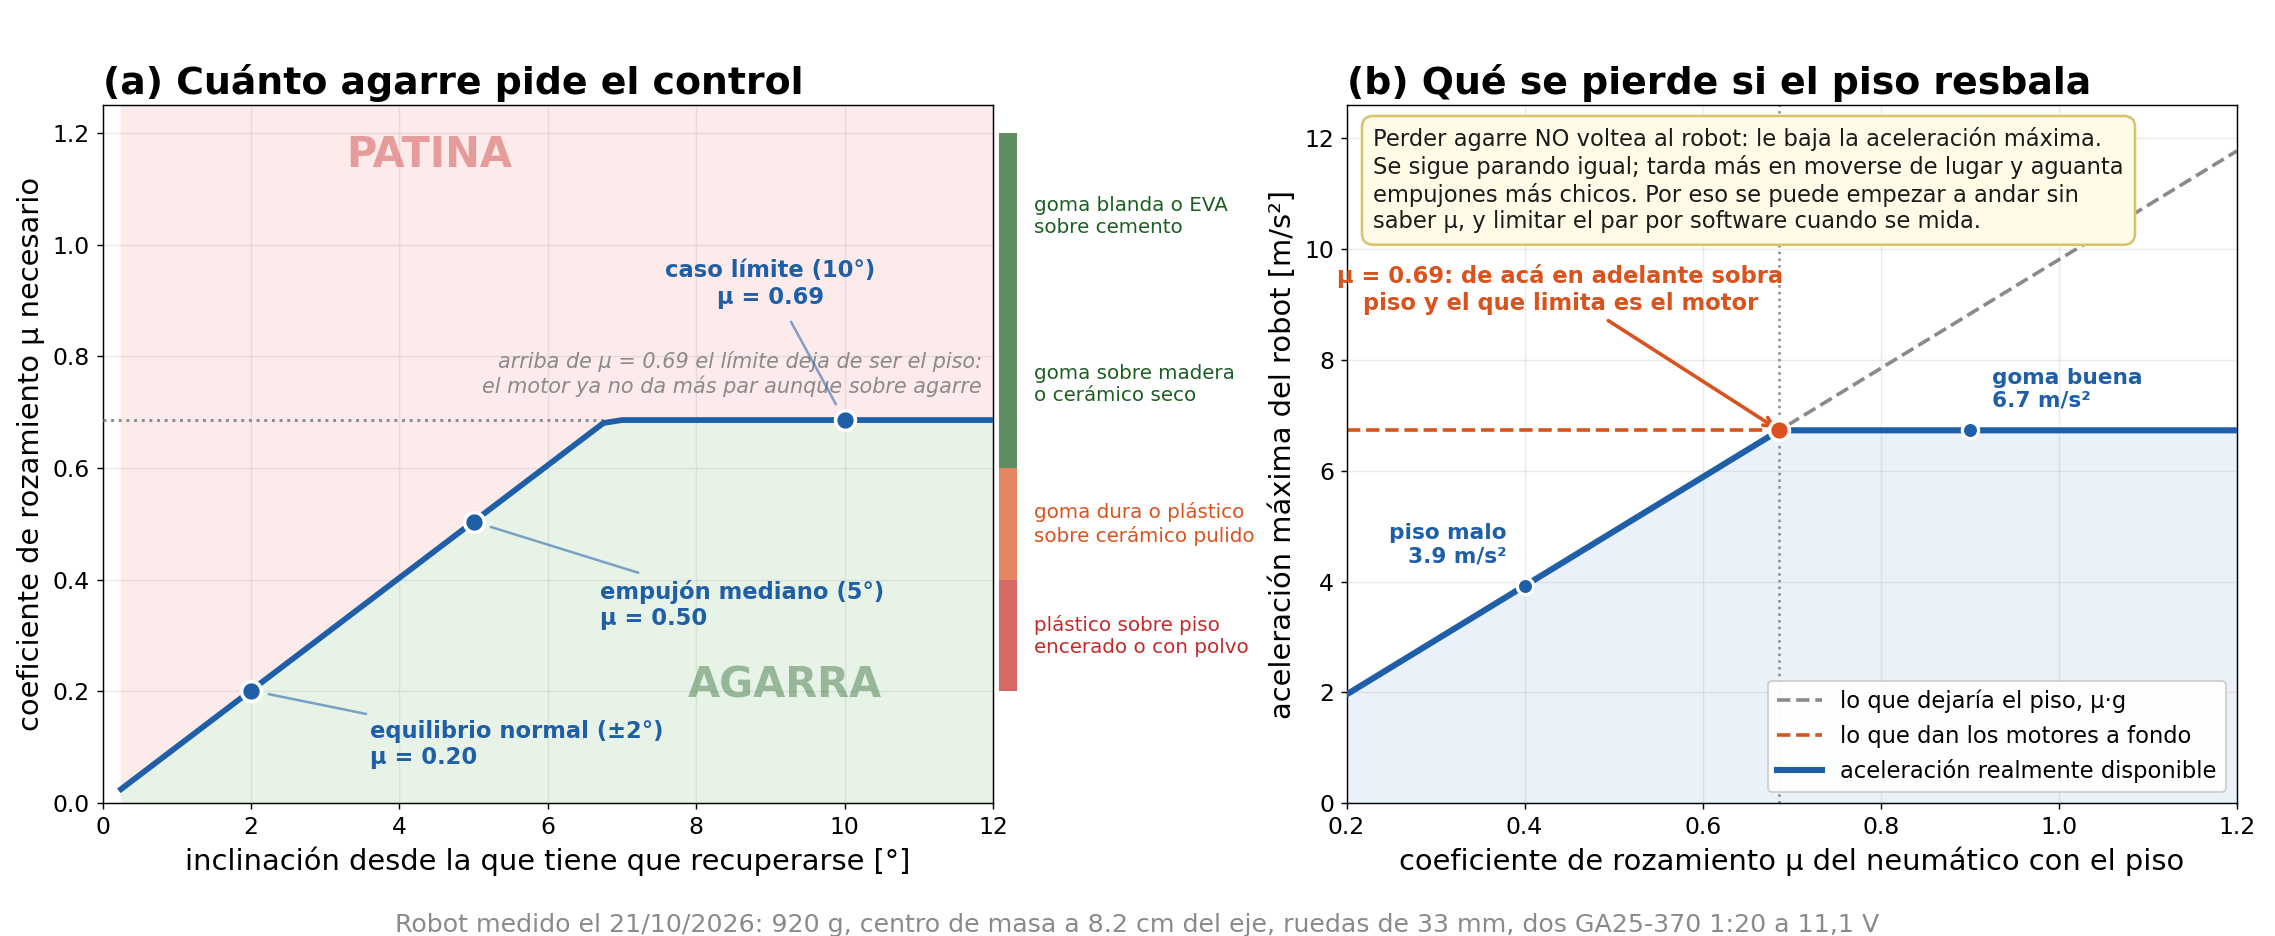
\includegraphics[width=\textwidth]{fig_traccion.png}
\captionof{figure}{Cuánto agarre pide el control en cada maniobra, y qué se pierde si el piso
resbala.}
\end{center}

% ===========================================================================
\chapter{El controlador: por qué LQR}\label{cap:lqr}
% ===========================================================================

\begin{idea}
Hay que estabilizar un sistema inestable con dos coordenadas y un solo actuador. El LQR no es
el único método que funciona, pero es el único que escala a ese problema sin que haya que
adivinar nada.
\end{idea}

\section{La justificación que se puede defender}

\begin{enumerate}[leftmargin=1.6em]
\item \textbf{Un PID no alcanza.} Un PID controla una salida. Acá hay dos coordenadas que
      importan, $x$ y $\varphi$, y un solo actuador. Realimentando sólo el ángulo el robot
      se equilibra pero \textbf{la posición queda siempre inestable}: se va caminando. Está
      verificado en el capítulo \ref{cap:simulink}.
\item \textbf{Con realimentación de estado hay que elegir cuatro ganancias a la vez.} Ubicar
      polos funciona, pero elegir cuatro polos de un sistema de cuarto orden a mano es
      adivinar. El LQR convierte esa elección en algo que se puede justificar: cuánto
      \emph{molesta} cada error y cuánta tensión se está dispuesto a gastar.
\item \textbf{La regla de Bryson le da sentido físico a los pesos.} Se pesa cada estado por
      el inverso del cuadrado de su valor máximo tolerable. Acá: 10 cm de error de posición,
      30 cm/s, $8^\circ$ de inclinación, 1 rad/s.
\item \textbf{El LQR regala márgenes.} La desigualdad de Kalman garantiza margen de fase
      $\geq 60^\circ$ y margen de ganancia infinito hacia arriba, \emph{por construcción}.
      Acá el margen de fase medido es $94^\circ$.
\end{enumerate}

\begin{ojo}
Para un sistema de una sola entrada, LQR y ubicación de polos dan \emph{exactamente} el mismo
controlador si se ubican los polos donde el LQR los puso (verificado a $10^{-12}$). Así que el
argumento a favor del LQR no puede ser sobre el resultado: es sobre el \textbf{método}. El LQR
te dice dónde poner los polos; ubicación de polos te pide que ya lo sepas.
\end{ojo}

\section{Los pesos, y una corrección que importó}

\begin{equation}
Q = \mathrm{diag}\!\left(\frac{1}{0{,}10^2},\ \frac{1}{0{,}30^2},\
\frac{1}{(8^\circ)^2},\ \frac{1}{1^2}\right)
= \mathrm{diag}(100{,}0,\ 11{,}1,\ 51{,}3,\ 1{,}0),
\qquad
R = \frac{f_R}{V_{bat}^2}.
\end{equation}

\begin{ojo}
Con la regla de Bryson pura ($f_R = 1$) el diseño es impecable en el papel y
\textbf{no sobrevive a la implementación}. Pone un polo en $-182$ s$^{-1}$ que no tiene nada
que ver con la física del robot (el más rápido de la planta es $-23{,}5$): es puro costo de
muestreo. Con un período de 5 ms, un paso de retardo y el filtro de 20 Hz que la cuantización
del encoder obliga, el lazo queda \textbf{inestable}, con radio espectral 1{,}163.

Con $f_R = 4$: radio espectral 0{,}986, el polo caro baja a $-93$ y el margen de muestreo pasa
de 1{,}2$\times$ a 2{,}5$\times$ y el ruido del encoder cae de 5{,}4 a 3{,}0 V. Cuesta un 6\%
de tiempo de respuesta: el escalón de 30 cm pasa de 1{,}70 a 1{,}80 s. \textbf{Es una de las decisiones más importantes del proyecto}, y no aparece en
ningún libro: aparece al simular la implementación real.
\end{ojo}

\section{El controlador que quedó}

\begin{equation}
U = -K\,(z - z_{ref}), \qquad
K = \begin{bmatrix} -55{,}50 & -53{,}12 & -90{,}17 & -11{,}44 \end{bmatrix}
\end{equation}

en voltios por (m, m/s, rad, rad/s).

\begin{center}
\begin{tabular}{@{}lr@{}}
\toprule
Polos a lazo cerrado & $-93{,}08$;\ $-7{,}17$;\ $-2{,}51 \pm 1{,}24i$ \\
Tiempo de asentamiento & 1{,}60 s \\
Margen de fase & $93{,}9^\circ$ a 80{,}9 rad/s \\
Pico de sensibilidad $\|S\|_\infty$ & 1{,}00 \\
\bottomrule
\end{tabular}
\end{center}

Un pico de sensibilidad de 1{,}00 es lo mejor que se puede pedir: significa que el lazo no
amplifica ninguna perturbación en ninguna frecuencia.

% ===========================================================================
\chapter{Simulink: cómo correrlo}\label{cap:simulink}
% ===========================================================================

\begin{idea}
Hay un solo archivo que abrir. Construye el modelo si falta, lo simula, lo compara contra una
integración independiente en MATLAB, y deja figura en \texttt{resultados/}. El recorrido
bloque por bloque del diagrama está en una guía aparte, \texttt{guia\_simulink.pdf}, que es la
versión corta de este documento enfocada sólo en Simulink.
\end{idea}

\section{El archivo que se abre}

\begin{center}
\texttt{simulacion/segway\_completo/INICIAR\_SEGWAY.m}
\end{center}

Se abre y se pulsa \textbf{Run}. No hace falta nada más: el script agrega las rutas, lee los
parámetros, diseña el LQR, arma las tablas de cada postura de las patas, construye el
\texttt{.slx} si no existe, simula y verifica.

\section{Cómo está armado el diagrama}

Seis etapas de izquierda a derecha, cada una en su área:

\begin{center}
\small
\begin{tabular}{@{}lp{11.2cm}@{}}
\toprule
\textbf{Etapa} & \textbf{Qué hace} \\
\midrule
Consignas & adónde se le pide ir y en qué postura poner las patas \\
Control & $U = -K\,(z_{medido} - z_{ref})$, y el reparto a las dos ruedas (con la entrada de giro
en cero) \\
Actuadores & los \textbf{cuatro motores}, cada uno en su bloque: dos GA25-370 de rueda (batería,
constante de par y contraelectromotriz) y dos DS3240 de pata (lazo de posición con tope de
velocidad y topes mecánicos) \\
Planta & la física, en cuatro etapas numeradas: el par que llega a la rueda, los coeficientes
según la postura, las dos ecuaciones de Newton--Euler por separado, y el despeje de las dos
aceleraciones por Cramer \\
Sensores & encoders e IMU, cada uno con su fuente de ruido (hoy en cero). La IMU mide el ángulo
del \emph{chasis} y el firmware le suma $\delta_G$ para recuperar $\varphi$ \\
Registro & saca las señales al workspace \\
\bottomrule
\end{tabular}
\end{center}

La planta \textbf{no} está armada con matrices anónimas: cada señal lleva el nombre de lo que es
---\emph{suma de fuerzas}, \emph{suma de momentos}, \emph{masa efectiva}, \emph{inercia del
cuerpo}, \emph{acople}--- y es exactamente la ecuación \eqref{eq:planta} escrita en bloques.

\section{Las variables en el workspace}

El archivo es un \emph{script}, no una función. Eso es a propósito: todo lo que calcula queda
en el \textbf{workspace base}, que es justamente de donde Simulink lee sus parámetros. La
\textbf{sección 2} del script junta todo lo que conviene tocar:

\begin{center}
\small
\begin{tabular}{@{}llp{7.4cm}@{}}
\toprule
\textbf{Variable} & \textbf{Por defecto} & \textbf{Qué cambia} \\
\midrule
\texttt{postura\_deg} & 25 & en qué postura se diseña el control \\
\texttt{phi0} & $5^\circ$ & de qué inclinación arranca \\
\texttt{x\_destino} & 0,30 m & adónde se le pide ir (0 = quedarse quieto) \\
\texttt{theta\_pata\_fin} & igual a la inicial & si las patas se mueven o no \\
\texttt{giro\_ref} & 0 & diferencia de tensión entre las dos ruedas \\
\texttt{ruido\_imu\_angulo}, \ldots & 0 & ruido de cada sensor \\
\texttt{sesgo\_imu} & 0 & error constante de la IMU \\
\texttt{compensar\_delta\_G} & 1 & si el firmware corrige el ángulo según la postura \\
\bottomrule
\end{tabular}
\end{center}

Al terminar quedan además \texttt{p} (la planta en SI), \texttt{motor}, \texttt{C} (el diseño
del control, con $A$, $B$, $Q$, $R$, polos y márgenes), \texttt{K}, y los resultados
\texttt{z\_sl}, \texttt{z\_med}, \texttt{U\_sl}, \texttt{tau\_sl} y \texttt{th\_sl}.

\section{Lo que da}

\begin{center}
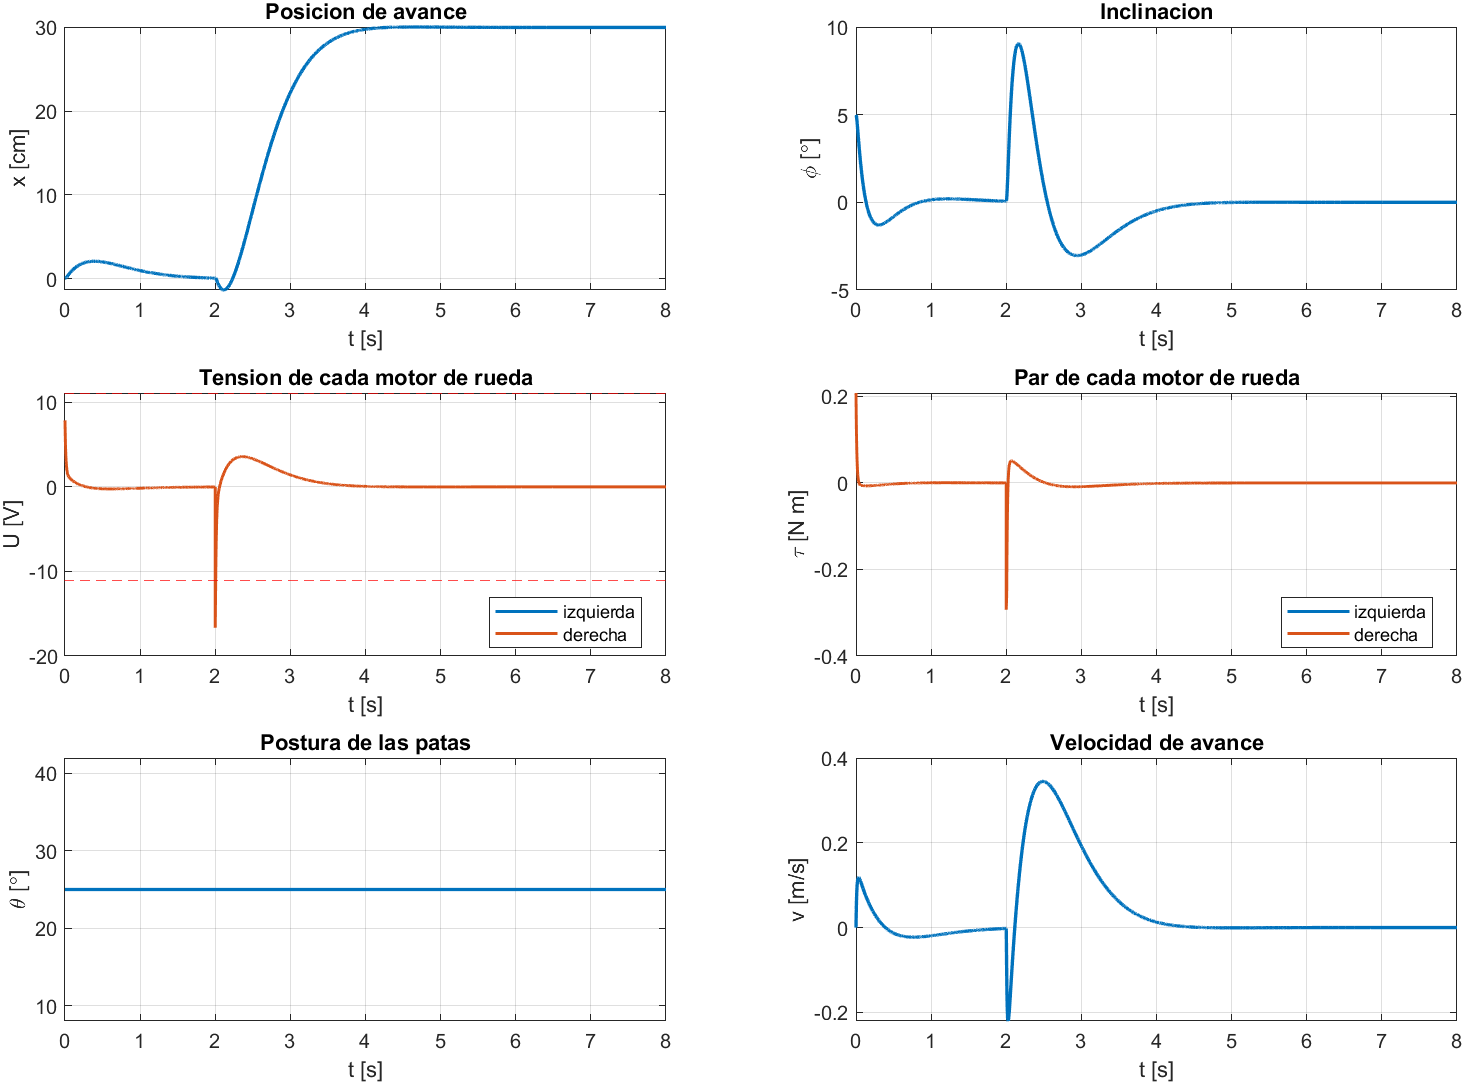
\includegraphics[width=\textwidth]{respuesta_segway.png}
\captionof{figure}{Las dos cosas que se le piden al robot: quedarse parado (arranca inclinado
$5^\circ$) y moverse 30 cm hacia adelante a partir de $t = 2$ s. Fijate en la inclinación: al
arrancar se va a $+9^\circ$, o sea \textbf{hacia adelante}, que es hacia donde avanza. Y justo
antes la tensión pega un pico \emph{negativo}: es el empujón hacia atrás que hace falta para
tirar el cuerpo hacia adelante.}
\end{center}

\begin{center}
\begin{tabular}{@{}lr@{}}
\toprule
\multicolumn{2}{@{}l}{\textbf{a) Quedarse parado, arrancando inclinado $5^\circ$}}\\
Inclinación a los 2 s & $0{,}064^\circ$ \\
Cuánto se corrió del lugar & 20{,}6 mm \\
\midrule
\multicolumn{2}{@{}l}{\textbf{b) Ir a 30 cm hacia adelante}}\\
Error final & 0{,}0 mm \\
Retroceso antes de avanzar & 14{,}2 mm \\
Inclinación máxima & $+9{,}05^\circ$ (hacia adelante) \\
Tiempo al 98\% & 1{,}80 s \\
\midrule
\multicolumn{2}{@{}l}{\textbf{Común}}\\
Tensión que pide el control & 16{,}7 V (la batería da 11{,}1: el resto se satura) \\
Tiempo saturando el agarre & 0\% \\
Normal mínima & 9{,}1 N (la rueda nunca despega) \\
\bottomrule
\end{tabular}
\end{center}

\section{Por qué se puede confiar en el resultado}

Simulink no se valida solo. El mismo problema se integra en paralelo con \texttt{ode45} sobre
una implementación \emph{independiente} de la planta, escrita a mano. Las dos coinciden en:

\begin{center}
\begin{tabular}{@{}lr@{}}
\toprule
$x$ & $1{,}4\times10^{-12}$ m \\
$v$ & $9{,}7\times10^{-11}$ m/s \\
$\varphi$ & $1{,}0\times10^{-11}$ rad \\
$\omega$ & $8{,}8\times10^{-10}$ rad/s \\
\bottomrule
\end{tabular}
\end{center}

Además hay una verificación de seis grupos que corre en los tests: simetría y definición
positiva de $M$, las matrices $A$ y $B$ contra diferencias finitas, el balance de potencia,
el balance horizontal de Newton y la deriva de energía sin fricción. Los seis pasan, y la
suite completa del proyecto está en \textbf{35 de 35}.

% ===========================================================================
\chapter{Qué pasa si las patas se mueven}\label{cap:patasmov}
% ===========================================================================

\begin{idea}
Todo lo anterior congela las patas. Si los dos servos pasan a ser actuadores, la altura del
péndulo cambia mientras el robot se equilibra. La pregunta es si eso rompe el control.
La respuesta corta: \textbf{no}, pero hay que corregir una cosa en el firmware.
\end{idea}

\section{Cuánto cambia la planta}

\begin{center}
\begin{tabular}{@{}rrrrrr@{}}
\toprule
\textbf{Postura} & \textbf{Alto CoM} & \textbf{Brazo $\ell$} & \textbf{Polo} &
\textbf{$\delta_G$} & \textbf{$K_\varphi$} \\
$[^\circ]$ & [cm] & [cm] & [s$^{-1}$] & $[^\circ]$ & \\
\midrule
10 (plegada) & 7{,}9 & 3{,}93 & 7{,}14 & $-9{,}09$ & $-76{,}4$ \\
15 & 9{,}4 & 5{,}44 & 7{,}42 & $-6{,}10$ & $-81{,}8$ \\
20 & 10{,}8 & 6{,}84 & 7{,}43 & $-4{,}52$ & $-86{,}2$ \\
25 & 12{,}1 & 8{,}15 & 7{,}35 & $-3{,}58$ & $-90{,}2$ \\
30 & 13{,}4 & 9{,}40 & 7{,}21 & $-2{,}94$ & $-93{,}8$ \\
35 & 14{,}6 & 10{,}60 & 7{,}06 & $-2{,}41$ & $-97{,}2$ \\
40 (estirada) & 15{,}8 & 11{,}77 & 6{,}91 & $-1{,}78$ & $-100{,}4$ \\
\bottomrule
\end{tabular}
\end{center}

El centro de masa \textbf{se duplica} en altura, de 7{,}9 a 15{,}8 cm. Y sin embargo el polo
inestable se mueve apenas un 7\%, entre 6{,}91 y 7{,}43 s$^{-1}$, con el máximo en el medio.

\begin{idea}
La intuición de la escoba --- cuanto más larga, más fácil de equilibrar --- \textbf{no se
aplica acá}. Esa intuición vale para una masa puntual, donde el polo es $\sqrt{g/\ell}$. En
este robot la \emph{inercia propia del cuerpo} domina sobre el efecto péndulo, y los dos
efectos se compensan.

Dicho de otro modo: \textbf{las patas no sirven para equilibrar}. Sirven para dar despeje,
para amortiguar el aterrizaje (capítulo \ref{cap:din}) y para levantarse.
\end{idea}

\section{¿Hace falta un controlador distinto en cada postura?}

No. Aplicando el $K$ diseñado a $25^\circ$ sobre la planta de cada postura:

\begin{center}
\begin{tabular}{@{}rrrr@{}}
\toprule
\textbf{Postura} & \textbf{Polo lento} & \textbf{¿Estable?} & \textbf{Asentamiento} \\
\midrule
$10^\circ$ & $-1{,}37$ s$^{-1}$ & sí & 2{,}93 s \\
$25^\circ$ & $-2{,}51$ s$^{-1}$ & sí & 1{,}60 s \\
$40^\circ$ & $-2{,}83$ s$^{-1}$ & sí & 1{,}41 s \\
\bottomrule
\end{tabular}
\end{center}

Es estable en todo el rango, con margen de fase entre $84^\circ$ y $94^\circ$. El precio de
usar un solo $K$ es que, con la pata totalmente plegada, el robot tarda un 51\% más en
asentarse. Es un precio barato comparado con la complejidad de programar \emph{gain
scheduling}.

\begin{idea}
\textbf{Recomendación: un solo $K$, el de la postura media.} Si más adelante se quiere afinar,
lo que más se gana es subir $|K_\varphi|$ y $|K_\omega|$ a medida que la pata se estira: de
punta a punta cambian un 31\% y un 48\% respectivamente. Las ganancias de posición y velocidad
no cambian nada.
\end{idea}

\section{Lo que sí hay que corregir}

\begin{ojo}
Mirá la columna $\delta_G$ de la tabla: va de $-9{,}09^\circ$ con la pata plegada a
$-1{,}78^\circ$ con la pata estirada. $\delta_G$ es lo que hay entre el ángulo del chasis ---
que es lo que mide la IMU --- y $\varphi$, que es lo que necesita el control.

O sea: \textbf{al mover la pata, el cero del ángulo se corre $7{,}31^\circ$}. Si el firmware
no lo corrige, el control va a creer que el robot está inclinado cuando no lo está.
\end{ojo}

Simulado con el modelo de Simulink completo, con los servos reales estirando la pata de
$10^\circ$ a $40^\circ$:

\begin{center}
\begin{tabular}{@{}lrr@{}}
\toprule
& \textbf{Se corre} & \textbf{Inclinación máxima} \\
\midrule
Sin compensar & 207 mm & $7{,}5^\circ$ \\
\textbf{Compensando} & \textbf{0 mm} & \textbf{$0{,}0^\circ$} \\
\bottomrule
\end{tabular}
\end{center}

No se cae en ninguno de los dos casos --- el robot aguanta ---, pero sin compensar se corre
21 cm del lugar cada vez que cambia de postura. La corrección es una línea:

\begin{center}
\texttt{phi = angulo\_imu + delta\_G(postura\_del\_servo)}
\end{center}

y $\delta_G$ es una función conocida de la postura, que el servo ya sabe porque es él quien la
comanda. Se tabula una vez y se interpola.

\begin{ojo}
Esta simulación interpola los coeficientes de la planta entre posturas. Es una aproximación:
el modelo exacto con patas móviles necesita $\theta$ como tercera coordenada del estado, y
ese modelo todavía no está hecho. Lo que sí es exacto es la tabla de la sección anterior,
porque cada fila es un modelo congelado completo. En otras palabras: \emph{que las ganancias
casi no cambian} está firme; \emph{que cuesta 21 cm} es una estimación.
\end{ojo}

% ===========================================================================
\chapter{Lo que falta medir}\label{cap:falta}
% ===========================================================================

\begin{idea}
El modelo está cerrado y verificado, pero descansa sobre un puñado de números que nadie midió.
Este capítulo dice cuáles son y cuánto cambiaría la conclusión si estuvieran mal.
\end{idea}

\begin{center}
\small
\begin{tabular}{@{}llp{7.0cm}@{}}
\toprule
\textbf{\#} & \textbf{Qué} & \textbf{Si está mal, cambia\ldots} \\
\midrule
M-1 & $\mu$ del neumático & \textbf{todo el margen de tracción}. Es el único parámetro
sin ninguna cota \\
M-6 & rigidez del neumático & \textbf{todo el pico del golpe al aterrizar} \\
M-7 & rigidez de la pata armada & el pico del golpe, otra vez: en serie manda la más blanda \\
M-2 & par real y rendimiento del reductor & el par disponible $\pm25\%$ \\
M-3 & resolución del encoder & el filtro de velocidad y el ruido que entra al control \\
M-4 & masa de rueda y motor & \textcolor{verdep}{\textbf{medida el 22/10}}: rueda 50 g, motor 96 g \\
M-5 & inercia del rotor & el coeficiente de avance, hasta un 43\% \\
\bottomrule
\end{tabular}
\end{center}

\section{Por qué el diseño igual es robusto}

Ya están medidas todas las masas. Se movió cada una de las suposiciones que quedan ---el
rendimiento del reductor, la inercia del rotor, la resistencia del motor--- de a una. El polo
inestable se queda entre 7{,}07 y 7{,}59 s$^{-1}$ y la ganancia $K_\varphi$ varía menos de
$\pm6\%$. El diseño del control no depende de ninguna de ellas.

\textbf{Lo único realmente indeterminado es si patina o no.} Y ahí la buena noticia es que el
equilibrio normal --- inclinarse dos o tres grados --- pide apenas $\mu = 0{,}19$, que lo da
hasta un piso encerado. Recuperarse de $5^\circ$ pide 0{,}46 y de $10^\circ$, 0{,}66.

\begin{idea}
Perder agarre \textbf{no voltea al robot}: le baja la aceleración máxima y la tolerancia a
empujones. Por eso se puede armar y probar el equilibrio sin saber $\mu$, y medirlo después.
\end{idea}

\section{Cómo se mide $\mu$}

\begin{center}
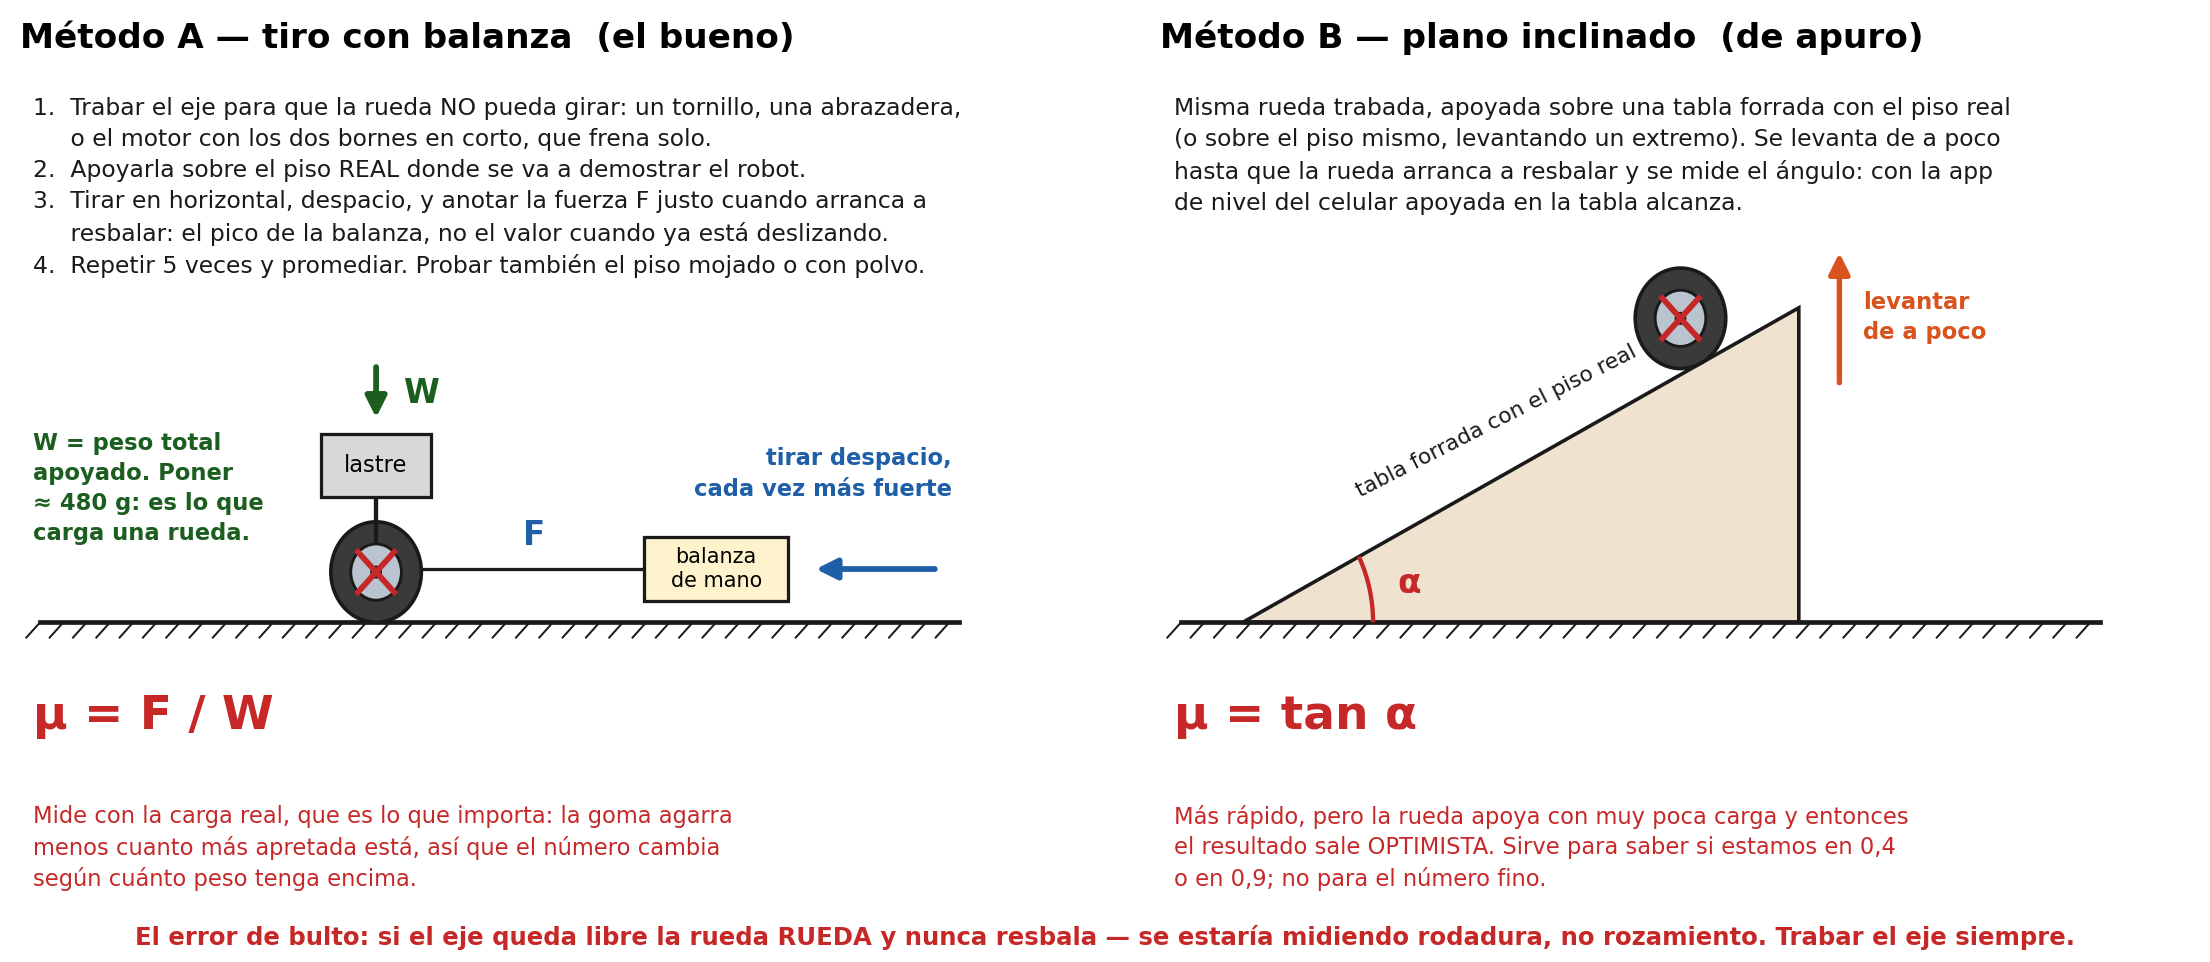
\includegraphics[width=\textwidth]{fig_ensayo_mu.png}
\captionof{figure}{Los dos métodos. Alcanza con una rueda sola: no hace falta el robot
armado.}
\end{center}

El plan completo de ensayos, con los siete y en qué orden hacerlos, está en
\begin{center}
\texttt{docs/gestion/2026-10-21-plan-de-ensayos.md}
\end{center}


% ===========================================================================
\chapter{Diseño mecánico e iteración constructiva}\label{cap:mec}
% ===========================================================================

\begin{idea}
El diseño mecánico en SolidWorks pasó por tres iteraciones completas hasta converger en una
arquitectura modular impresa en PLA: mecanismo de cuatro barras a escala 80 con eslabón
acoplador rígido en horquilla, cabina central portante para los dos servos DS3240 MG y las
dos placas electrónicas (potencia y lógica), y sujeción rígida de los motorreductores
GA25-370 con encoder en el extremo inferior de cada pata.
\end{idea}

\section{Evolución geométrica: de Hoeken al cuatro barras de 3.ª iteración}

El proyecto comenzó explorando un mecanismo de línea aproximada de Hoeken con eslabón
flexible. Esa primera aproximación se descartó en agosto de 2026 por dos razones técnicas:
la concentración de tensiones en la bisagra flexible impresa en FDM y la dificultad de
garantizar simetría bilateral entre ambas patas bajo carga dinámica.

Se adoptó en su lugar un \textbf{mecanismo plano de cuatro barras articuladas} $ABCD$ con
extensión rígida del acoplador hasta el eje de rueda $P$ (\texttt{eslabon\_cdp}). A partir de un
barrido numérico de proporciones adimensionales se seleccionó la familia
$1{,}40 : 1{,}35 : 0{,}51 : 1{,}40$ con ángulo interno del acoplador $\delta = 164^\circ$ y
bancada $AB$ inclinada $45^\circ$ respecto de la horizontal:

\begin{center}
\begin{tabular}{@{}llll@{}}
\toprule
\textbf{Iteración} & \textbf{Escala y rasgos constructivos} & \textbf{Hallazgo de ingeniería} & \textbf{Estado} \\
\midrule
1.ª iteración & Bancada $AB = 80\ud{mm}$, barras a escala 100 & Al mezclar escalas se perdía la trayectoria cuasi-rectilínea de $P$ & Descartada \\
2.ª iteración & Barras llevadas a escala 80 ($AD=112$, $BC=108$, $CD=40{,}8$, $DP=112\ud{mm}$) & Recupera la trayectoria casi recta del eje de rueda ($107\ud{mm}$ de carrera vertical) & Base de \texttt{parametros\_fisicos.m} \\
\textbf{3.ª iteración} & Rediseño estructural de \texttt{eslabon\_cdp} (v4), \texttt{eslabon\_BC} doble (interno/externo) y \texttt{cabeza\_v4} & Elimina torsión fuera del plano, aloja el GA25-370 real y reserva el volumen \texttt{pcb\_max\_size} & \textbf{Construida y ensayada} \\
\bottomrule
\end{tabular}
\end{center}

En la tercera iteración (\texttt{diseño\_mecanico/3er\_iteracion/} y \texttt{chasis nuevo/}), el
balancín $BC$ se desdobló en dos caras paralelas (\texttt{eslabon\_BC\_interna} y
\texttt{eslabon\_BC\_externa}) que abrazan tanto la cabina como el acoplador $CDP$, trabajando a
corte doble sobre los pasadores y aumentando drásticamente la rigidez frente al alabeo cuando
una rueda pisa desparejo respecto de la otra.

\section{Elasticidad estructural en serie: por qué el PLA protege al servo}

En el capítulo \ref{cap:din} se calculó que, si toda la estructura de la pata fuera
infinitamente rígida y el único elemento elástico fuera la banda de rodadura del neumático
($k_n \approx 30\ud{kN/m}$), la fase A del aterrizaje desde un escalón de $18\ud{cm}$ (los
primeros $\sim 3\ud{ms}$ en que se frena en seco la masa no suspendida de $146\ud{g}$ de rueda y
motor) generaría un pico impulsivo de hasta $\mathbf{421\ud{N}}$ sobre el eje del servo $A$.

Sin embargo, una estructura impresa en PLA no es un cuerpo rígido frente a impactos de
milisegundos. A partir de la masa medida de la manivela $AD$ ($30\ud{g}$ en $112\ud{mm}$ de
longitud) se deduce una sección transversal efectiva media de $233\ud{mm^2}$. Considerando el
módulo elástico efectivo del PLA impreso con perímetros y relleno ($E \approx 2{,}0\text{--}2{,}8\ud{GPa}$)
y la flexión combinada de la manivela, los pasadores y la carcasa, la rigidez estructural
equivalente vista desde el contacto resulta del orden de:
\[
k_{\text{pata}} \in [4,\; 15]\ud{kN/m}
\]
es decir, \textbf{del mismo orden o más blanda que el propio neumático}. Al actuar ambos
elementos como resortes en serie, la rigidez efectiva $k_{\text{eq}}$ queda dominada por el
término más flexible:
\[
k_{\text{eq}} = \frac{k_n\,k_{\text{pata}}}{k_n + k_{\text{pata}}}
\qquad\Longrightarrow\qquad
F_{\text{pico}} = \sqrt{2\,E_{\text{imp}}\,k_{\text{eq}}}
\]

\begin{center}
\begin{tabular}{@{}rrrr@{}}
\toprule
\textbf{Rigidez de la pata $k_{\text{pata}}$} & \textbf{Escalón de 2 cm} & \textbf{Escalón de 5 cm} & \textbf{Escalón de 18 cm} \\
\midrule
$\infty$ (cota rígida teórica) & $140\ud{N}$ & $221\ud{N}$ & $421\ud{N}$ \\
$15\ud{kN/m}$ (estructura rígida en PLA) & $81\ud{N}$ & $128\ud{N}$ & $243\ud{N}$ \\
$\mathbf{8\ud{kN/m}}$ \textbf{(valor nominal estimado)} & $\mathbf{64\ud{N}}$ & $\mathbf{101\ud{N}}$ & $\mathbf{193\ud{N}}$ \\
$5\ud{kN/m}$ (estructura más flexible) & $53\ud{N}$ & $84\ud{N}$ & $159\ud{N}$ \\
\bottomrule
\end{tabular}
\end{center}

\begin{idea}
La elasticidad propia de los eslabones impresos en PLA reduce la fuerza pico de impacto sobre
el eje del servo a \textbf{menos de la mitad} ($193\ud{N}$ frente a $421\ud{N}$ en un escalón de
$18\ud{cm}$, y apenas $64\ud{N}$ en un desnivel de $2\ud{cm}$). Aun así, $193\ud{N}$ equivale a
quince veces la carga estática en reposo ($12{,}2\ud{N}$), por lo que la regla constructiva se
mantiene intacta: el pasador en $A$ debe descargar radialmente sobre la pared de la cabina y
dejar que el estriado del servo transmita únicamente par torsor.
\end{idea}

\section{Dispositivo de banco y retención por trinquete}

Para realizar los ensayos de identificación, ajuste de signos de encoders y verificación del
lazo en vacío sin arriesgar la integridad del prototipo ante caídas, se diseñó un soporte de
mesa paramétrico en Python (\texttt{build123d}, ítem \texttt{BAN-001} del registro de ingeniería):
una prensa tipo sargento fijada al borde de la mesa con un brazo voladizo de $100\ud{mm}$, una
polea superior y un malacate con rueda de trinquete y uñeta elástica que suspende al robot
desde dos puntos separados $130\ud{mm}$ mediante un balancín ecualizador. La geometría se
verificó libre de interferencias en STEP/STL con una precarga controlada de $12{,}6\ud{mm^3}$
en la lámina elástica de retención.

% ===========================================================================
\chapter{Arquitectura electrónica y diseño de PCB}\label{cap:elec}
% ===========================================================================

\begin{idea}
La electrónica se dividió físicamente en dos placas impresas de una sola faz fabricadas por
transferencia térmica (\emph{plancha}): una \textbf{Placa de Potencia v0.7} ($124 \times 77\ud{mm}$)
y una \textbf{Placa de Lógica v0.6} ($95{,}25 \times 59{,}6\ud{mm}$), vinculadas por un cable
plano IDC de 16 vías (\texttt{J20}). Todos los integrados complejos se montan como módulos
comerciales verificados sobre zócalos codificados o pines soldados, reduciendo al mínimo los
componentes discretos y aislando las corrientes de potencia del microcontrolador.
\end{idea}

\section{Criterio de partición y evolución del hardware}

Durante las primeras pruebas de equilibrio y levantamiento de datos se utilizó un prototipo
de banco con un puente bipolar doble \textbf{L298N}. Ese ensayo permitió cuantificar en
condiciones reales su limitación principal: una caída interna de tensión de $\approx 2{,}0\ud{V}$
que reducía la excursión útil sobre los motores a $\sim 9{,}1\ud{V}$ con tensión nominal de
batería ($11{,}1\ud{V}$), obligando a incrementar las ganancias del LQR un $22\%$ (capítulo
\ref{cap:lqr} y sección \ref{sec:lqr_ajustado}).

Para la versión definitiva montada en la cabina (\texttt{segway\_v02} sobre placas v0.7/v0.6) se
migró a una arquitectura de potencia distribuida cuyos planos completos y guías de montaje se
incluyen en el apéndice \ref{ap:pcb}:

\begin{enumerate}[leftmargin=1.6em]
\item \textbf{Etapa de tracción por rueda (2 $\times$ DRV8871):} un puente H MOSFET por motor
      (\texttt{A3} y \texttt{A4}) con límite de corriente interno y una caída mucho menor que la del
      L298N bipolar, operados con PWM a $20\ud{kHz}$ en modo de decaimiento lento (\emph{slow decay} /
      frenado activo), que linealiza la respuesta par-comando cerca del origen.
\item \textbf{Alimentación independiente por servo (2 $\times$ UBEC de 6,0 V):} en la revisión
      v0.7 se asignó un regulador conmutado UBEC exclusivo para cada servo DS3240 MG
      (columnas \texttt{DER} en \texttt{J16}/\texttt{J14} e \texttt{IZQ} en \texttt{J19}/\texttt{J13}),
      respaldado cada uno por un capacitor electrolítico de baja ESR de $470\ud{\mu F}/16\ud{V}$
      (\texttt{C8} y \texttt{C9}). Esto evita que los picos de corriente de hasta $\sim 2{,}5\ud{A}$
      por servo al amortiguar un aterrizaje provoquen caídas de tensión cruzadas.
\item \textbf{Regulación lógica en doble escalón:} un convertidor \emph{buck} de $5\ud{V}$
      (\texttt{A8}) en la placa de potencia alimenta los sensores ópticos y envía el bus
      intermedio por el cable plano \texttt{J20} hacia la placa de lógica, donde un segundo
      \emph{buck} de $3{,}3\ud{V}$ (\texttt{A9}) alimenta el módulo \textbf{ESP32-S3 DevKitC-1
      N16R8} (\texttt{A1}), la IMU \textbf{MPU-6050} (\texttt{A2}) y los encoders magnéticos de
      cuadratura (\texttt{J7} y \texttt{J8}).
\end{enumerate}

\section{Esquema de protecciones y seguridad eléctrica}

Siguiendo el criterio de diseño adoptado por el equipo el 31/10/2026, se conservaron en placa
únicamente los componentes pasivos y de protección con función crítica demostrada:

\begin{center}
\small
\begin{tabular}{@{}llp{8.8cm}@{}}
\toprule
\textbf{Elemento} & \textbf{Valor / Tipo} & \textbf{Función de protección en el circuito} \\
\midrule
Fusible en línea + \texttt{F1} & $20\ud{A}$ cable / $15\ud{A}$ lento ATO & Protección general de la batería LiPo 3S contra cortocircuitos francos en barras, soportando el transitorio de arranque \\
\texttt{F2}, \texttt{F3} & $4\ud{A}$ mini (uno por rueda) & Corte individual ante rotor bloqueado o falla en corto de cada módulo DRV8871 \\
\texttt{F4} & $7{,}5\ud{A}$ mini & Protección conjunta de la entrada de ambos UBEC (\texttt{J15}) ante bloqueo mecánico simultáneo de los dos servos ($\sim 5\ud{A}$) \\
\texttt{F5} & $1\ud{A}$ mini & Protección dedicada de la rama de lógica, medidor \texttt{INA226} y cable plano \texttt{J20} \\
\texttt{D1} & TVS \texttt{SA15A} (\texttt{VM\_BUS}) & Supresión de sobretensiones transitorias regeneradas por los motores durante inversiones bruscas de marcha \\
\texttt{C1}, \texttt{C3} & $470\ud{\mu F}/35\ud{V}$ + $10\ud{\mu F}$ cer. & Reserva local exigida por los DRV8871 y filtrado de alta frecuencia en terminales de salida del BMS \\
\texttt{R5}, \texttt{R6} & $1\ud{k\Omega}$ en serie (PWM servos) & Limita la corriente hacia los GPIO de la ESP32 si un conector JR de servo se enchufa desplazado un pin (evita inyectar $6\ud{V}$ directos al riel de $3{,}3\ud{V}$) \\
\texttt{R41}, \texttt{R42} & Divisor $10\ud{k\Omega} / 15\ud{k\Omega}$ (1\%) & Atenúa la salida analógica del sensor de distancia Sharp GP2Y0A60SZLF (hasta $3{,}6\ud{V}$ en operación o $5\ud{V}$ ante falla de cableado) a un máximo seguro de $2{,}2\text{--}3{,}0\ud{V}$ en \texttt{GPIO3} \\
Codificación física & Pin cortado en \texttt{A1} y \texttt{A2} & Se corta el pin 24 (\texttt{GPIO43}) de la ESP32-S3 y el pin 5 del MPU-6050 cegando el zócalo para impedir mecánicamente la inserción invertida \\
\bottomrule
\end{tabular}
\end{center}

\begin{ojo}
Los módulos reguladores \texttt{A8}/\texttt{A9} y los sensores de corriente \texttt{A5}--\texttt{A7}
no admiten inversión de montaje sin destruirse; por decisión de diseño van \textbf{soldados en
forma permanente} tras verificar continuidad y orientación. Asimismo, si se emplea un
interruptor de parada sin contacto auxiliar, el conector \texttt{J4} de aviso a la ESP32 debe
puentearse: abierto, el firmware interpreta parada de emergencia activa e inhibe el armado.
\end{ojo}

\section{Instrumentación de energía en el bus $\text{I}^2\text{C}$}

En la placa de potencia se integraron tres monitores digitales sobre el mismo bus $\text{I}^2\text{C}$
de $400\ud{kHz}$ (\texttt{SDA=GPIO8}, \texttt{SCL=GPIO9}) que utiliza la IMU:

\begin{itemize}[leftmargin=1.5em]
\item \textbf{Dos módulos INA219 (\texttt{A5} en \texttt{0x40} y \texttt{A6} en \texttt{0x41}, puente \texttt{A0}):}
      ubicados aguas arriba de cada DRV8871, miden la tensión de entrada al driver y la
      corriente absorbida (positiva en tracción, negativa durante frenado regenerativo).
\item \textbf{Un módulo INA226 (\texttt{A7} en \texttt{0x44}):} mide la tensión general de la
      batería LiPo y el consumo de la rama lógica (hasta $0{,}82\ud{A}$). Durante la puesta en
      marcha del 6/11 se detectó un desvío sistemático en la lectura de tensión del módulo
      INA226 ($12{,}86\ud{V}$ frente a $12{,}20\text{--}12{,}25\ud{V}$ reales medidos por ambos
      INA219), originado en la continuidad interna entre \texttt{VBS} e \texttt{IN-} de la placa
      comercial; se corrigió por software mediante calibración afín
      (\texttt{INA226\_V\_GANANCIA} e \texttt{INA226\_V\_CERO}) contrastada contra los INA219.
\end{itemize}

% ===========================================================================
\chapter{Firmware en tiempo real (ESP-IDF) y estación de mando}\label{cap:fw}
% ===========================================================================

\begin{idea}
El software embebido se desarrolló en C sobre ESP-IDF v6.1 y FreeRTOS con tick de $1\ud{kHz}$.
Toda la matemática de estimación, odometría, control LQR, movimiento y maniobra de escalón está
escrita en \textbf{C puro sin dependencias del hardware} (\texttt{components/control/}), lo que
permite compilar exactamente el mismo código fuente en la PC para correr suites de pruebas
unitarias y simulaciones no lineales antes de tocar el robot.
\end{idea}

\section{Arquitectura concurrente en FreeRTOS y determinismo temporal}

Para garantizar que el período de muestreo $T_s = 5\ud{ms}$ ($200\ud{Hz}$) no sufra
variaciones (\emph{jitter}) por el tráfico WiFi o la impresión por consola USB, el firmware
separa estrictamente el procesamiento en los dos núcleos del ESP32-S3:

\begin{center}
\begin{tabular}{@{}llllp{6.6cm}@{}}
\toprule
\textbf{Tarea} & \textbf{Núcleo} & \textbf{Período} & \textbf{Prioridad} & \textbf{Secuencia determinística de ejecución} \\
\midrule
\texttt{control\_task} & Core 1 & $5\ud{ms}$ ($200\ud{Hz}$) & Máxima ($\text{MAX}-2$) & Vacía cola de comandos $\to$ lee IMU y Sharp $\to$ actualiza filtro de actitud y odometría $\to$ evalúa supervisor $\to$ ejecuta LQR / maniobra $\to$ actualiza PWM de motores y rampas de servos $\to$ si sobran $> \text{INA\_MARGEN\_US}$, lee un registro INA $\to$ publica telemetría \\
\texttt{comms\_task} & Core 0 & $20\ud{ms}$ ($50\ud{Hz}$) & Baja ($\text{IDLE}+2$) & Lee último estado del buzón sin bloquear $\to$ transmite línea CSV por USB-Serial-JTAG y UDP (\texttt{:4210}) $\to$ parsea comandos entrantes por USB y UDP (\texttt{:4211}) \\
\bottomrule
\end{tabular}
\end{center}

La comunicación inter-tareas prescinde por completo de variables globales compartidas y de
\emph{mutex}: los comandos bajan por una cola FIFO de 8 elementos que \texttt{control\_task}
consume únicamente al comienzo del ciclo, y la telemetría sube por una cola de 1 elemento con
sobrescritura (\texttt{xQueueOverwrite}). Cada ciclo mide su duración real en microsegundos con
\texttt{esp\_timer\_get\_time()} e informa en vivo el peor tiempo de ventana (\texttt{loop\_us\_max})
y el contador de excesos (\texttt{overruns}). Incluso sumando la lectura escalonada de los
medidores INA a 40 registros por segundo, el peor tiempo de ciclo medido en placa es de
$4{,}3\ud{ms}$ sobre los $5{,}0\ud{ms}$ disponibles, con \textbf{0 excesos de ciclo}.

\begin{center}
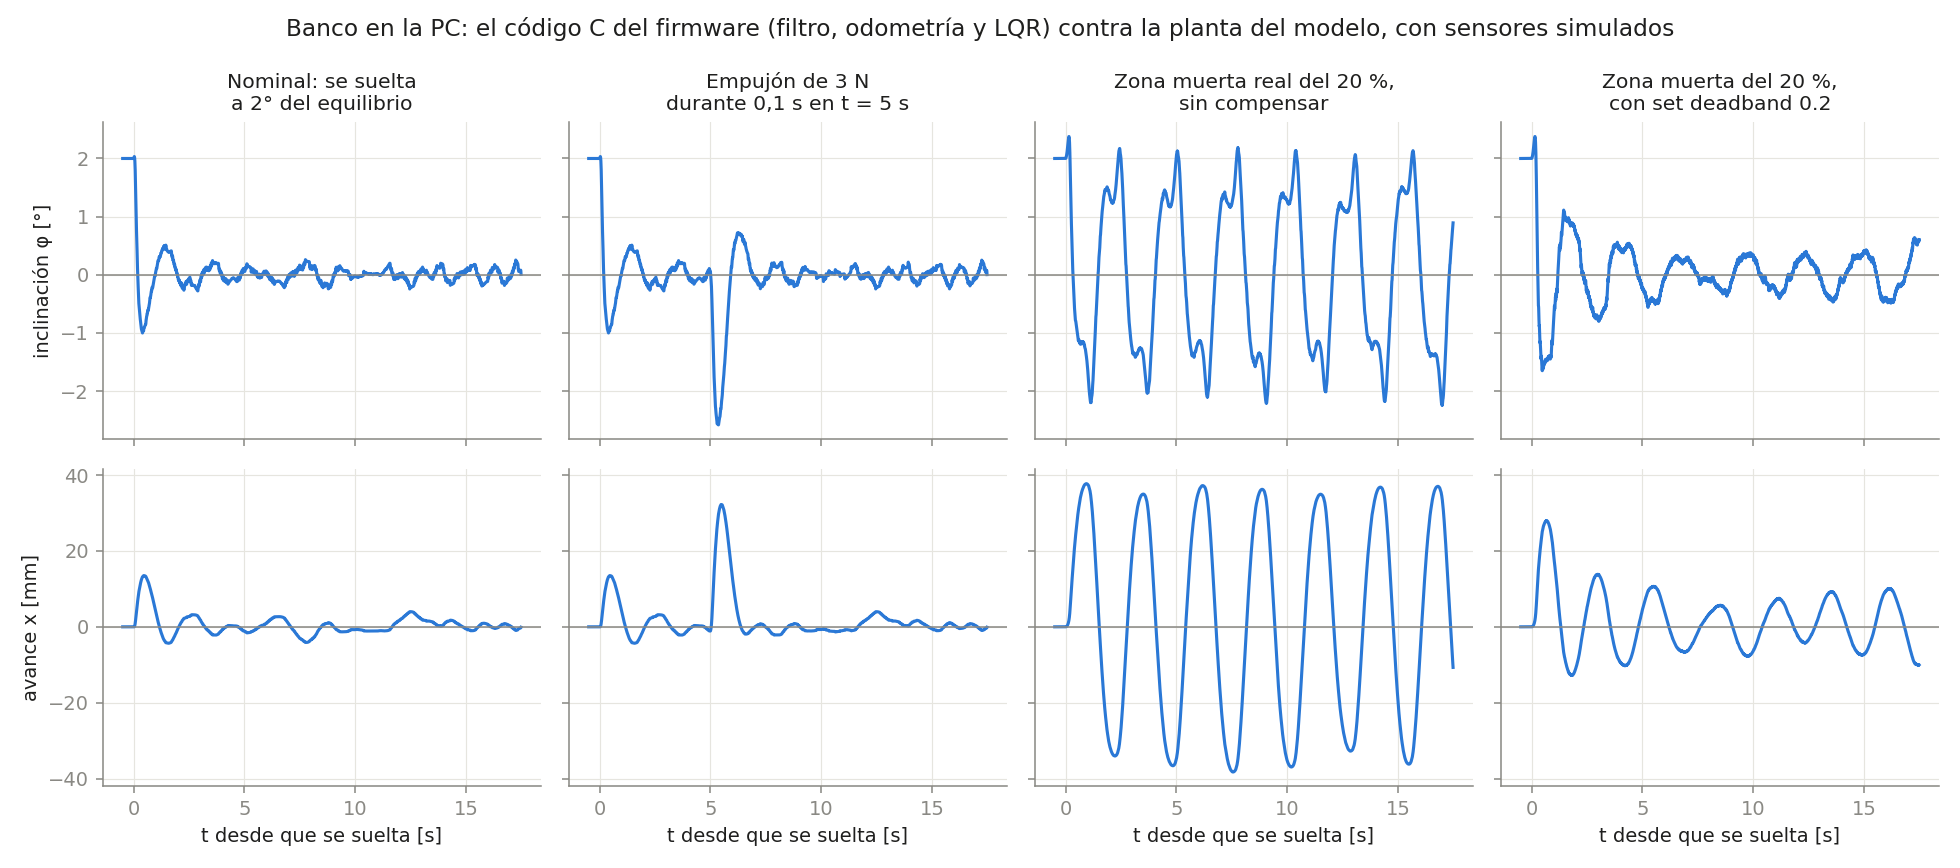
\includegraphics[width=0.92\textwidth]{banco_lqr.png}
\captionof{figure}{Verificación en PC (\texttt{banco\_lqr.c}): el código C exacto del firmware
(filtro complementario, odometría y LQR discreto a $200\ud{Hz}$) corriendo contra la planta
exportada desde MATLAB.}
\end{center}

\section{Estimación, odometría compensada y hallazgos del lazo real}

El cierre exitoso del lazo sobre el prototipo físico entre el 29/10 y el 3/11 dejó cinco
enseñanzas de ingeniería de control que no aparecen en un modelo ideal de libro:

\begin{enumerate}[leftmargin=1.6em]
\item \textbf{Odometría respecto del piso (\texttt{odometry.c}):} los encoders en cuadratura
      (leídos por hardware mediante el periférico \texttt{PCNT} en modo $\times 4$) miden el
      giro de la rueda \emph{respecto de la pata}, no respecto del piso. Si el robot se inclina
      un ángulo $\varphi$ sin desplazarse, el encoder cuenta giro. Por ello, la posición real
      del contacto se reconstruye sumando la inclinación del cuerpo:
      \[
      x = r\,\bigl(\theta_{\text{enc}} + \varphi\bigr)
      \]
      Por la misma razón física (cero de fase no mínima), en las pruebas con las ruedas en el
      aire \textbf{deben anularse $k_x$ y $k_v$}: sin la reacción del suelo que invierta el
      cabeceo, el lazo de posición acelera las ruedas indefinidamente en el mismo sentido.
\item \textbf{Filtro rechaza banda (\emph{notch}) a 7,5 Hz:} en el primer ensayo de equilibrio
      real (29/10), el robot presentaba una oscilación estructural propia de $7\text{--}8\ud{Hz}$
      que la derivada $\omega$ realimentaba hasta saturar el puente H de tope a tope. Un
      pasabajos convencional a $9\text{--}11\ud{Hz}$ introducía retardo de fase y hacía
      hamacarse al robot; la solución definitiva fue un \textbf{filtro rechaza banda centrado en
      $7{,}5\ud{Hz}$} (\texttt{set notch 7.5}), que suprimió la resonancia sin degradar el
      margen de fase del LQR.
\item \textbf{Doble zona muerta estática/dinámica (\texttt{deadband} vs.\ \texttt{dbmov}):} los
      motorreductores requieren un comando mínimo de $\approx 0{,}14\text{--}0{,}16$ de PWM
      para vencer la fricción seca en reposo. Sin compensación de zona muerta, el robot no
      sostiene la posición $x$ cuando está quieto; pero al desplazarse con el joystick, aplicar
      ese salto discontinuo en cada cruce por cero de $u$ generaba sacudones. Desde el 3/11 el
      firmware implementa dos umbrales: \texttt{deadband = 0.16} con el robot quieto y
      \texttt{dbmov = 0} en movimiento.
\item \textbf{Seguimiento de velocidad con consigna flotante (\texttt{xlibre = 1}) y prealimentación (\texttt{ff}):}
      cuando la referencia de posición se calculaba como la integral rígida de la velocidad
      pedida, el robot debía adelantarse $10\text{--}22\ud{cm}$ a la consigna para poder
      inclinarse y avanzar, y al soltar el stick retrocedía bruscamente para devolver esa
      diferencia. Con \texttt{xlibre = 1}, durante el movimiento el LQR regula únicamente la
      velocidad (la referencia $x_{\text{ref}}$ acompaña al robot) más un término anticipado
      $u_{\text{ff}} = \texttt{ff}\cdot v_{\text{ref}}$, y recién fija la posición final cuando
      la rampa de frenado termina y $|v|$ cae a cero.
\item \textbf{Inmunidad a caída libre en la IMU:} originalmente el driver del MPU-6050
      interpretaba $\|\boldsymbol{a}\| < 1\ud{m/s^2}$ como desconexión del sensor y pasaba a
      \texttt{FAULT} en $25\ud{ms}$. Durante el vuelo balístico al bajar un escalón ($\sim 190\ud{ms}$
      en ingravidez aparente), eso apagaba los motores en el aire. Desde el 3/11 una aceleración
      baja inferior a $0{,}6\ud{s}$ continuos no dispara falla: el estimador congela la
      corrección del acelerómetro y propaga la actitud exclusivamente con el giróscopo.
\end{enumerate}

\section{Estación de mando, telemetría web y control por DualShock 4}

Para operar el robot, diagnosticar sensores/actuadores y registrar ensayos a $200\ud{Hz}$, se
desarrolló una estación de tierra 100\% portable en Python estándar y HTML5/Canvas
(\texttt{Aplicacion/}, figura \ref{fig:hmi_banco}):

\begin{itemize}[leftmargin=1.5em]
\item \textbf{Arquitectura de doble puente (\texttt{puente.py} + \texttt{joystick.py}):} el
      servidor HTTP (\texttt{:8000}) recibe la telemetría UDP del robot (\texttt{:4210}), la
      distribuye al navegador por Server-Sent Events (SSE) y almacena automáticamente en disco
      los registros de alta velocidad (\texttt{registros/bajada\_*.csv}) que el robot transmite
      al finalizar cada maniobra de escalón. En paralelo, \texttt{joystick.py} (\texttt{:8001})
      lee el mando \textbf{PS4 DualShock 4 directamente por protocolo nativo HID}
      (\texttt{hid.dll} en Windows), lo que garantiza una tasa constante de $25\ud{Hz}$ por UDP
      incluso si el navegador pasa a segundo plano.
\item \textbf{Interfaz en cinco vistas:} \emph{Mando/Conducción} (HUD interactivo con modos de
      1 o 2 sticks conmutables con \texttt{OPTIONS}, pasos de $2^\circ$ en las patas entre
      $0^\circ$ y $30^\circ$ con \texttt{L1}/\texttt{R1}, armado con $\times$, corte de
      emergencia con $\bigcirc$, bajada de escalón con $\triangle$ y parada controlada con
      $\square$), \emph{Banco de pruebas} (prueba individual de cada sensor y actuador),
      \emph{Energía} (estado de carga SoC, autonomía restante y corrientes de los tres INA),
      \emph{Gráficos} (osciloscopio multicanal con cursor) y \emph{Configuración}.
\end{itemize}

\begin{center}
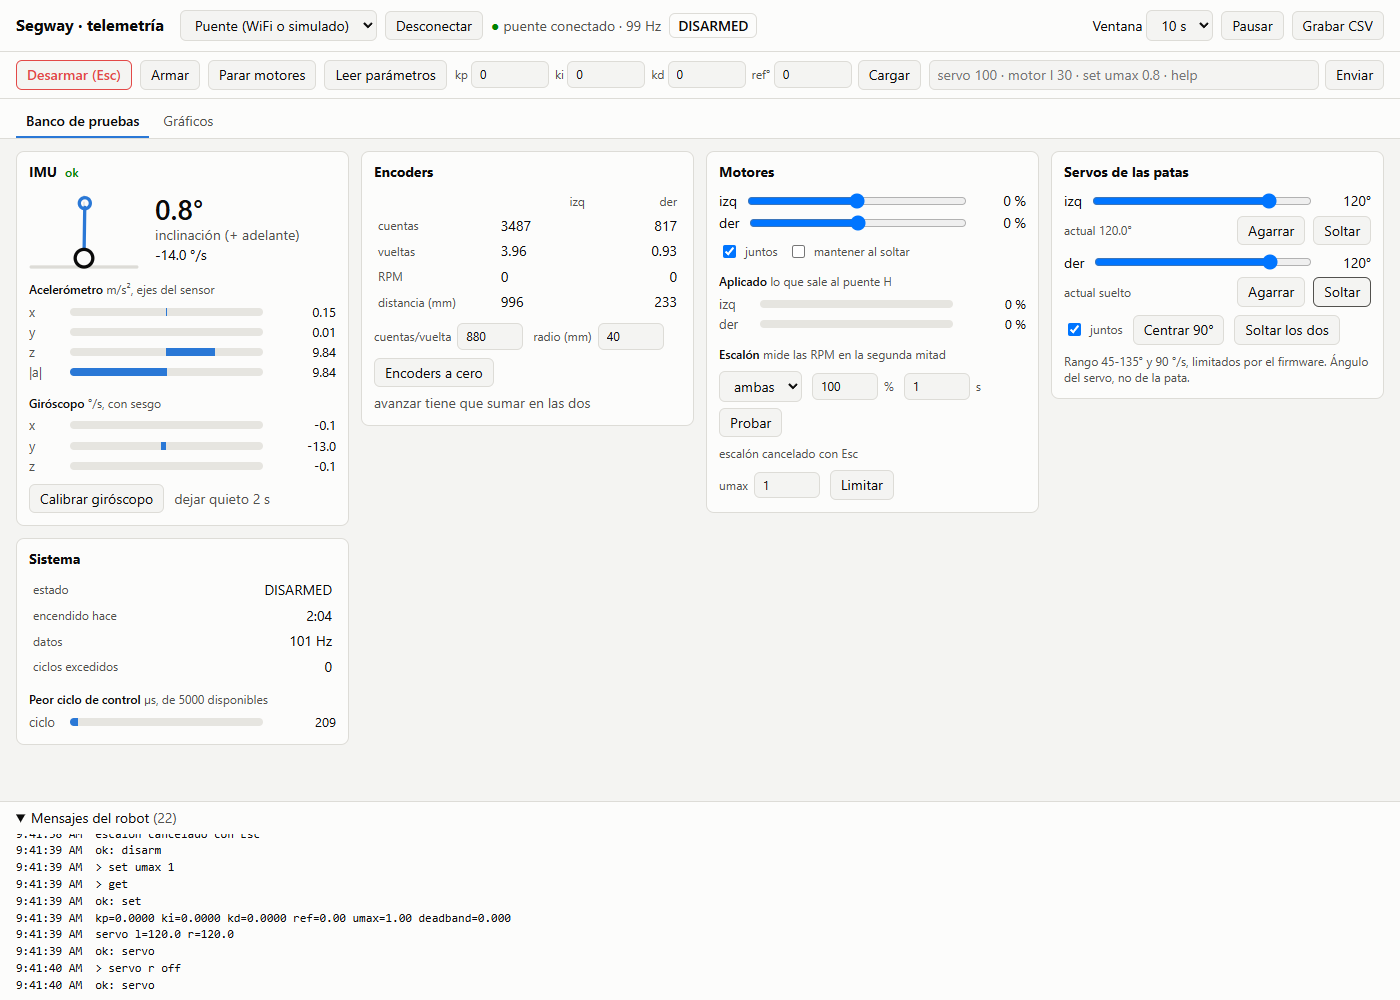
\includegraphics[width=0.95\textwidth]{banco_de_pruebas.png}
\captionof{figure}{Interfaz web de telemetría, diagnóstico y conducción (\texttt{Aplicacion/}):
vista del banco de pruebas e inspección de sensores y actuadores en tiempo real.}\label{fig:hmi_banco}
\end{center}

% ===========================================================================
\chapter{Identificación experimental y ajuste del modelo (Teoría vs.\ Realidad)}\label{cap:ajuste}
% ===========================================================================

\begin{idea}
El 3 de noviembre de 2026 se enfrentó el modelo teórico contra el robot real equilibrando en el
piso por WiFi. Con dos experimentos sistemáticos ---la curva estática de equilibrio en 13
alturas de pata y la respuesta dinámica a una onda cuadrada en 4 posturas--- se identificaron
los desvíos constructivos reales del prototipo. El error de predicción del ángulo de
equilibrio bajó veinte veces: de $\mathbf{1{,}52^\circ}$ a $\mathbf{0{,}08^\circ\;\text{rms}}$.
\end{idea}

\section{Protocolo de ensayo en lazo cerrado}

Usando la herramienta automatizada \texttt{firmware/herramientas/sesion\_placa.py}, con la
batería LiPo medida en $11{,}9\ud{V}$, se ejecutaron dos campañas de adquisición sin intervención
manual:

\begin{enumerate}[leftmargin=1.6em]
\item \textbf{Identificación estática (\texttt{medir\_equilibrio}):} con el robot equilibrando en
      el lugar, se barrió el ángulo comandado de las patas desde $0^\circ$ hasta $30^\circ$ en
      pasos de $2{,}5^\circ$ (13 posturas), realizando cuatro pasadas completas (dos subiendo y
      dos bajando, 48 registros de $12\ud{s}$ cada uno). Promediar las ramas ascendente y
      descendente permitió separar la curva geométrica pura de la \textbf{histéresis mecánica}
      ($\sim 0{,}9^\circ$ de diferencia entre subir y bajar, causada por la banda muerta de
      $3\ud{\mu s} \equiv 0{,}27^\circ$ del servo DS3240 y la holgura de los pasadores).
\item \textbf{Identificación dinámica (\texttt{identificar}):} se inyectó una onda cuadrada de
      $\pm 1{,}5^\circ$ en la referencia de inclinación ($2{,}08\ud{s}$ por semiperíodo, 5 ciclos
      completos) manteniendo las patas fijas en $25^\circ$, $20^\circ$, $10^\circ$ y $0^\circ$,
      provocando excursiones de $\pm 60\text{--}80\ud{mm}$ en posición y $\pm 3\text{--}5^\circ$
      en cabeceo.
\end{enumerate}

\begin{center}
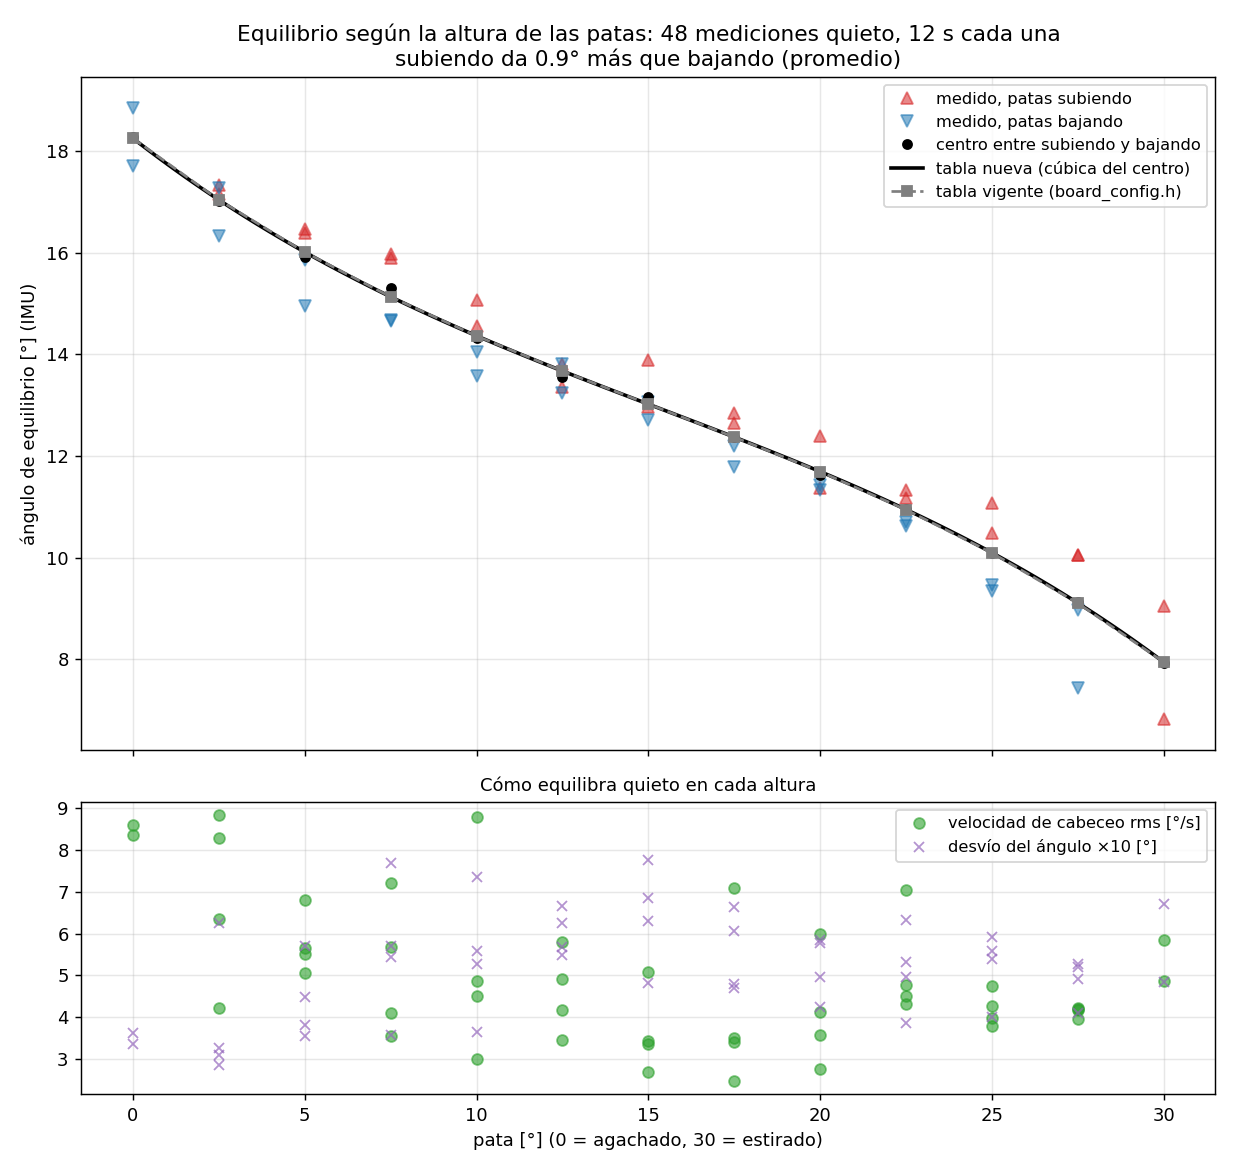
\includegraphics[width=0.88\textwidth]{equilibrio_patas_2026-11-03.png}
\captionof{figure}{Medición experimental del ángulo de equilibrio en función de la postura de
las patas (48 ensayos por WiFi, dos pasadas subiendo y dos bajando) y curva cúbica central
incorporada al firmware.}
\end{center}

\section{Deducción de los parámetros físicos reales}

En equilibrio estático ($\ddot{x}=0$, $\ddot{\varphi}=0$), el centro de masa total del robot
debe ubicarse exactamente sobre la vertical del eje de la rueda, por lo que el ángulo leído
por la IMU responde a la ley geométrica:
\[
\theta_{\text{IMU}}^{\text{eq}}(\theta_{\text{pata}}) =
\delta_{\text{imu}} + \operatorname{atan2}\!\bigl(-c_x(\theta_{\text{pata}}),\; c_z(\theta_{\text{pata}})\bigr)
\]
donde $(c_x, c_z)$ son las coordenadas del baricentro conjunto respecto del eje $P$. La curva
medida en el robot resultó significativamente más empinada hacia los $30^\circ$ que la predicha
por el modelo nominal. Como se demuestra en \texttt{modelado/ajuste/ajustar\_equilibrio.m}, ni
un simple offset de montaje de la IMU ni un corrimiento del centro de masa de la cabina pueden
curvar la pendiente de esa manera; \textbf{lo único que explica el aumento de pendiente cerca
de $30^\circ$ es que la pata real trabaja $10{,}4^\circ$ más estirada que lo supuesto},
acercándose antes a la singularidad geométrica (punto muerto) del cuadrilátero articulado:

\begin{center}
\small
\begin{tabular}{@{}lrrrrl@{}}
\toprule
\textbf{Hipótesis de ajuste estático} & \textbf{IMU [$^\circ$]} & \textbf{Caja $x$ [mm]} & \textbf{Caja $z$ [mm]} & \textbf{Cero pata [$^\circ$]} & \textbf{Error rms / máx [$^\circ$]} \\
\midrule
Modelo nominal previo & $9{,}80$ & $0{,}0$ & $0{,}0$ & $0{,}00$ & $1{,}52^\circ$ / $3{,}65^\circ$ \\
Ajustando solo offset de IMU & $8{,}82$ & $0{,}0$ & $0{,}0$ & $0{,}00$ & $1{,}17^\circ$ / $2{,}67^\circ$ \\
IMU + corrimiento horizontal de caja & $6{,}70$ & $-4{,}3$ & $0{,}0$ & $0{,}00$ & $0{,}90^\circ$ / $1{,}86^\circ$ \\
IMU + cero de la pata & $8{,}27$ & $0{,}0$ & $0{,}0$ & $-1{,}86$ & $1{,}06^\circ$ / $2{,}37^\circ$ \\
\textbf{IMU + caja $x$ + cero de la pata (elegido)} & $\mathbf{4{,}17}$ & $\mathbf{-19{,}3}$ & $\mathbf{0{,}0}$ & $\mathbf{+10{,}41}$ & $\mathbf{0{,}10^\circ}$ / $\mathbf{0{,}22^\circ}$ \\
\bottomrule
\end{tabular}
\end{center}

A continuación, se replicó el ensayo de onda cuadrada en \texttt{banco\_identificacion.c}
(ejecutando el código C exacto del firmware con su filtro de actitud, odometría, rechaza banda
y zona muerta) y se barrió una grilla sobre los parámetros electromecánicos. El ajuste dinámico
confirmó de manera independiente el mismo corrimiento de $+10{,}4^\circ$ en el cero de las patas
y cerró los parámetros del tren de tracción (variante \texttt{'ajustada'} en
\texttt{parametros\_fisicos.m}):

\begin{center}
\small
\begin{tabular}{@{}llll@{}}
\toprule
\textbf{Parámetro físico} & \textbf{Modelo nominal} & \textbf{Modelo ajustado} & \textbf{Evidencia experimental} \\
\midrule
Postura del modelo con pata en $0^\circ$ (\texttt{pata\_cero}) & $10{,}0^\circ$ & $\mathbf{20{,}4^\circ}$ & Curvatura de equilibrio + respuesta en $0^\circ$ \\
Baricentro horizontal de la caja (\texttt{corr\_caja}) & $+7{,}4\ud{mm}$ (delante de $A$) & $\mathbf{-11{,}9\ud{mm}}$ ($19{,}3\ud{mm}$ atrás) & Equilibrio estático en 13 alturas \\
Inclinación de montaje de la IMU (\texttt{imu\_delta\_deg}) & $9{,}8^\circ$ & $\mathbf{4{,}2^\circ}$ & Regresión conjunta de equilibrio \\
Velocidad de vacío del motor (\texttt{w\_nl\_motor\_rpm}) & $300\ud{rpm}$ ($K_t$ mayor) & $\mathbf{350\ud{rpm}}$ ($K_t, K_e$ $-14\%$) & Ensayo en vacío \texttt{MED-005} y onda cuadrada \\
Relación de reducción del motorreductor ($N$) & $20{,}00$ & $\mathbf{20{,}43}$ & Conteo de pulsos de encoder en 10 vueltas \\
Tensión real de ensayo ($V_{\text{bat}}$ / motor con L298N) & $11{,}1\ud{V}$ / $9{,}1\ud{V}$ & $\mathbf{11{,}9\ud{V}}$ / $\mathbf{9{,}9\ud{V}}$ & Multímetro y amplitud de onda cuadrada \\
Zona muerta efectiva de tracción (\texttt{zona\_muerta\_motor}) & $0{,}17$ PWM & $\mathbf{0{,}14\;\text{PWM}}$ & Amplitud de ciclo límite en onda cuadrada \\
Banda muerta de posición del servo (\texttt{banda\_servo\_deg}) & $0^\circ$ & $\mathbf{0{,}27^\circ}$ ($3\ud{\mu s}$) & Hoja de datos DS3240 y escalones a $4\ud{^\circ/s}$ \\
\bottomrule
\end{tabular}
\end{center}

\begin{center}
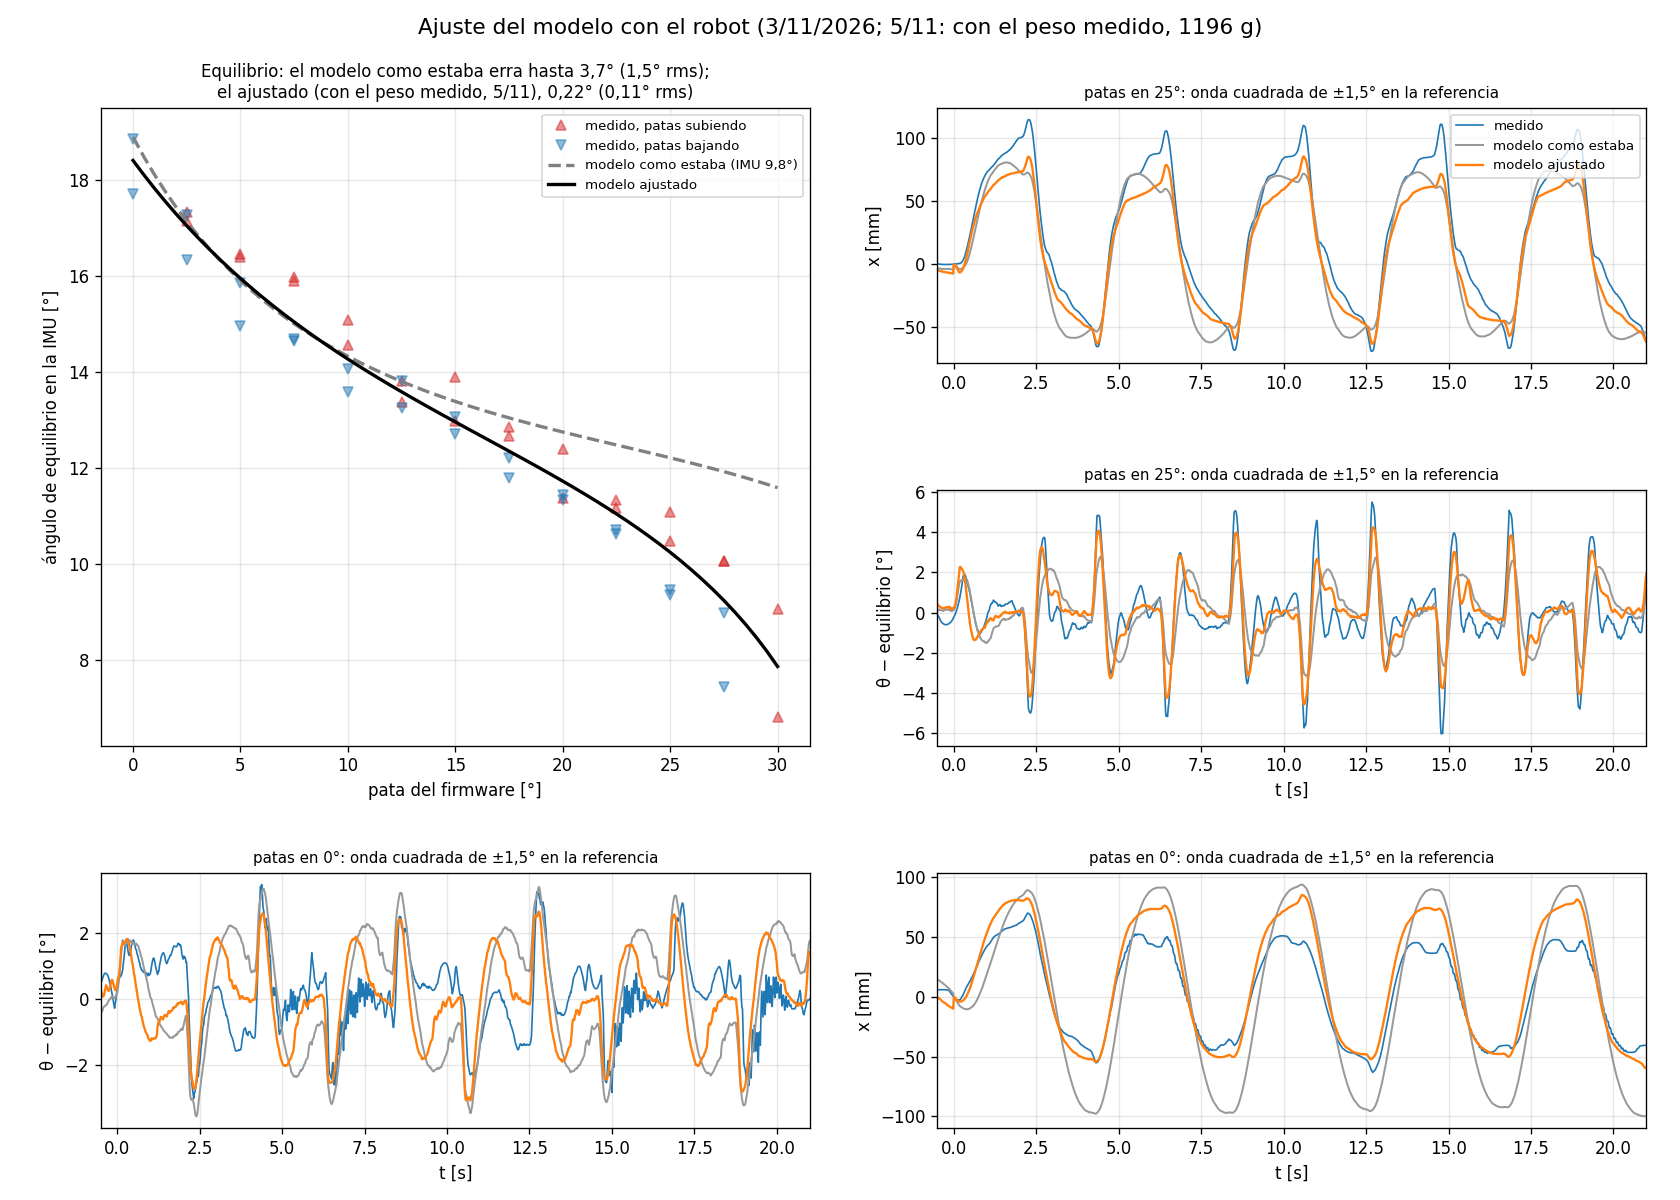
\includegraphics[width=0.98\textwidth]{fig_ajuste.png}
\captionof{figure}{Comparación entre las mediciones experimentales del robot (negro), el modelo
original (rojo) y el modelo ajustado (azul): curva estática de equilibrio (arriba) y respuesta
dinámica a la onda cuadrada de $\pm 1{,}5^\circ$ en las cuatro alturas de pata.}
\end{center}

Con estos ocho parámetros físicos actualizados, el error RMS del modelo frente a la onda
cuadrada medida cayó sistemáticamente en todas las posturas:

\begin{center}
\begin{tabular}{@{}rrr@{}}
\toprule
\textbf{Altura de patas} & \textbf{Error RMS de cabeceo (antes $\to$ ahora)} & \textbf{Error RMS de posición $x$ (antes $\to$ ahora)} \\
\midrule
$25^\circ$ & $1{,}45^\circ \;\longrightarrow\; \mathbf{0{,}78^\circ}$ & $21{,}4\ud{mm} \;\longrightarrow\; \mathbf{16{,}2\ud{mm}}$ \\
$20^\circ$ & $1{,}05^\circ \;\longrightarrow\; \mathbf{0{,}68^\circ}$ & $13{,}7\ud{mm} \;\longrightarrow\; \mathbf{11{,}1\ud{mm}}$ \\
$10^\circ$ & $1{,}32^\circ \;\longrightarrow\; \mathbf{0{,}96^\circ}$ & $15{,}6\ud{mm} \;\longrightarrow\; \mathbf{12{,}3\ud{mm}}$ \\
$0^\circ$  & $1{,}71^\circ \;\longrightarrow\; \mathbf{1{,}24^\circ}$ & $33{,}9\ud{mm} \;\longrightarrow\; \mathbf{11{,}6\ud{mm}}$ \\
\bottomrule
\end{tabular}
\end{center}

\section{Rediseño del LQR por altura de pata (\texttt{LQR\_TABLA})}\label{sec:lqr_ajustado}

Al estar las patas reales $10{,}4^\circ$ más extendidas y tener el motor de $350\ud{rpm}$ un
$27\%$ menos de amortiguamiento contraelectromotriz ($K_e K_t/R$), mantener las ganancias fijas
originales provocaba que el factor de amortiguamiento del modo de cabeceo cayera de
$\zeta = 0{,}98$ en $0^\circ$ a apenas $\mathbf{\zeta = 0{,}31}$ en $30^\circ$ (lo que explicó
las tres caídas sufridas por el robot real al ensayar la onda cuadrada en $30^\circ$).

Recalculando el regulador LQR con la planta ajustada (\texttt{simulacion/segway\_ajustado/ganancias\_ajustadas.m})
e incorporando la tabla \texttt{LQR\_TABLA} en el firmware (\texttt{set lqrpata 1} por defecto),
las ganancias de ángulo y velocidad angular crecen suavemente con la extensión de las patas y
mantienen la excursión de cabeceo acotada entre $5{,}1^\circ$ y $5{,}7^\circ$ en todo el rango:

\begin{center}
\begin{tabular}{@{}rrrrrr@{}}
\toprule
\textbf{Pata [$^\circ$]} & $\boldsymbol{k_x}$ \textbf{[1/m]} & $\boldsymbol{k_v}$ \textbf{[s/m]} & $\boldsymbol{k_\varphi}$ \textbf{[1/rad]} & $\boldsymbol{k_\omega}$ \textbf{[s/rad]} & \textbf{$\zeta$ con $K$ fijo anterior} \\
\midrule
$0$  & $1{,}50$ & $2{,}38$ & $3{,}73$ & $0{,}416$ & $0{,}98$ \\
$5$  & $1{,}50$ & $2{,}38$ & $3{,}96$ & $0{,}456$ & $1{,}00$ \\
$10$ & $1{,}50$ & $2{,}38$ & $4{,}17$ & $0{,}496$ & $0{,}91$ \\
$15$ & $1{,}50$ & $2{,}39$ & $4{,}36$ & $0{,}537$ & $0{,}72$ \\
$20$ & $1{,}50$ & $2{,}40$ & $4{,}54$ & $0{,}577$ & $0{,}57$ \\
$25$ & $1{,}50$ & $2{,}40$ & $4{,}71$ & $0{,}618$ & $0{,}43$ \\
$30$ & $1{,}50$ & $2{,}41$ & $4{,}88$ & $0{,}662$ & $\mathbf{0{,}31}$ \\
\bottomrule
\end{tabular}
\end{center}

\begin{center}
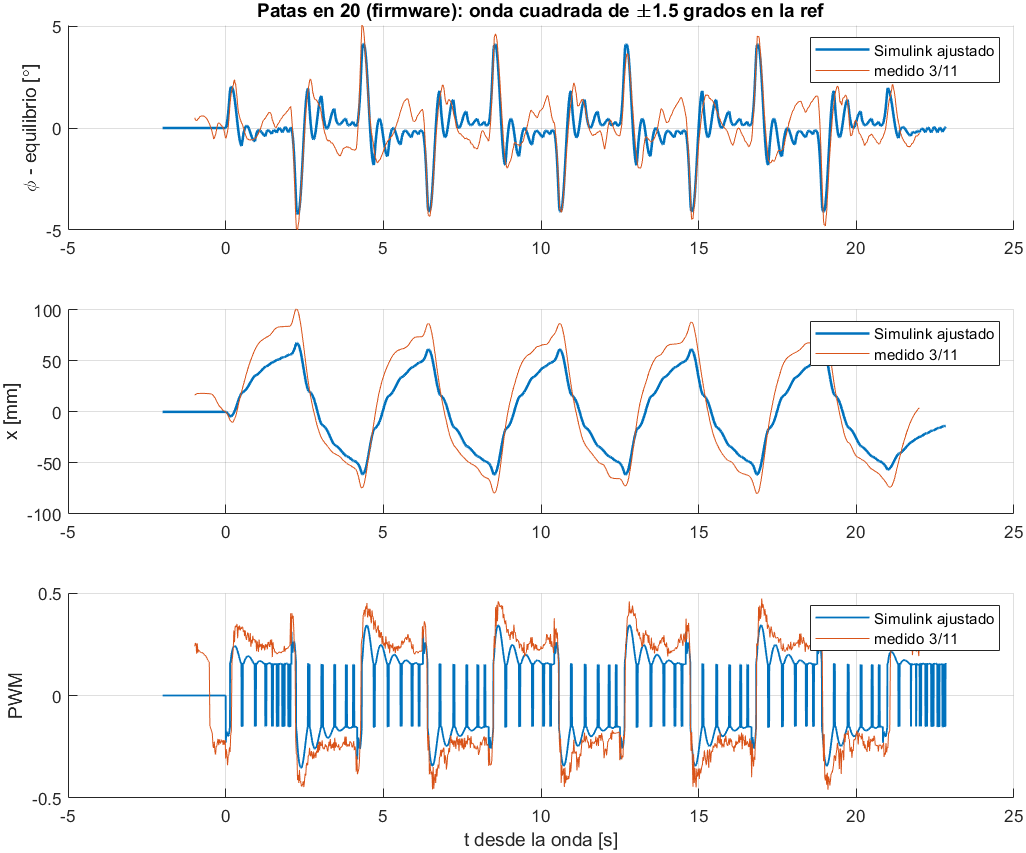
\includegraphics[width=0.88\textwidth]{onda_pata_20.png}
\captionof{figure}{Simulación en \texttt{segway\_ajustado.slx} de la respuesta a la onda cuadrada
con las patas en $20^\circ$, comparando el modelo ajustado contra el registro experimental.}
\end{center}

% ===========================================================================
\chapter{Maniobra de descenso de escalón y escalera con algoritmo genético}\label{cap:escalon}
% ===========================================================================

\begin{idea}
Bajar un escalón o una escalera es un problema dinámico híbrido donde el robot acelera hacia
atrás, pierde el contacto con el suelo, vuela en caída libre, impacta contra el escalón
inferior y debe absorber la energía con las patas sin que el frente de la cabina golpee el
borde saliente ni se sature el motor al recuperar la vertical. Para resolverlo sin romper el
prototipo, se construyó un simulador híbrido en C acoplado al código real de \texttt{maniobra.c},
un visor web interactivo y un optimizador evolutivo de dos islas.
\end{idea}

\section{Planta híbrida plana y validación de un escalón individual}

El banco \texttt{simulacion/escalon/banco\_escalon.c} integra las ecuaciones de cuerpo,
eslabones móviles de las patas y eje de ruedas con contacto unilateral viscoelástico y fricción
de Coulomb tanto para los neumáticos como para el contorno rectangular de la cabina, usando
la curva par-velocidad de los dos servos DS3240 ($2 \times 41\ud{kg\cdot cm}$, $327\ud{^\circ/s}$,
actualizados a $50\ud{Hz}$) y el modelo ajustado del capítulo \ref{cap:ajuste}.

Para el descenso de \textbf{un escalón aislado de 18 cm} (\texttt{un\_escalon.py}), el barrido
paramétrico y el análisis de robustez frente a 27 variaciones (tensión de batería de $10{,}5$
a $12{,}6\ud{V}$, zona muerta $0{,}10\text{--}0{,}18$, adherencia $\mu = 0{,}4$, servos al $80\%$,
corrimiento de equilibrio $\pm 0{,}75^\circ$, alturas de $16\text{--}20\ud{cm}$ e inercias
alteradas) demostraron una propiedad física fundamental:

\begin{ojo}
\textbf{En un escalón individual conviene mantener el LQR activo durante el vuelo
(\texttt{motor\_vuelo = 1}):} al abandonar el borde, el cuerpo queda $\sim 2^\circ$ detrás de
su equilibrio cabeceando hacia atrás. El LQR acelera las ruedas hacia atrás en el aire (hasta
$\sim 1\ud{m/s}$); por conservación del momento angular, el par de reacción endereza el chasis
durante la caída y, en el instante del toque, las ruedas más rápidas que el suelo empujan la
base hacia atrás devolviendo el centro de masa sobre el apoyo. Con esa estrategia (largada con
patas en $15^\circ$, velocidad pedida $0{,}54\ud{m/s}$, extensión a $30^\circ$ en el vuelo y
plegado amortiguado a $25^\circ$ a $300\ud{^\circ/s}$ al tocar), el robot supera con éxito
\textbf{25 de las 27 variaciones} y se detiene a $30\ud{cm}$ de la contrahuella.
\end{ojo}

\begin{center}
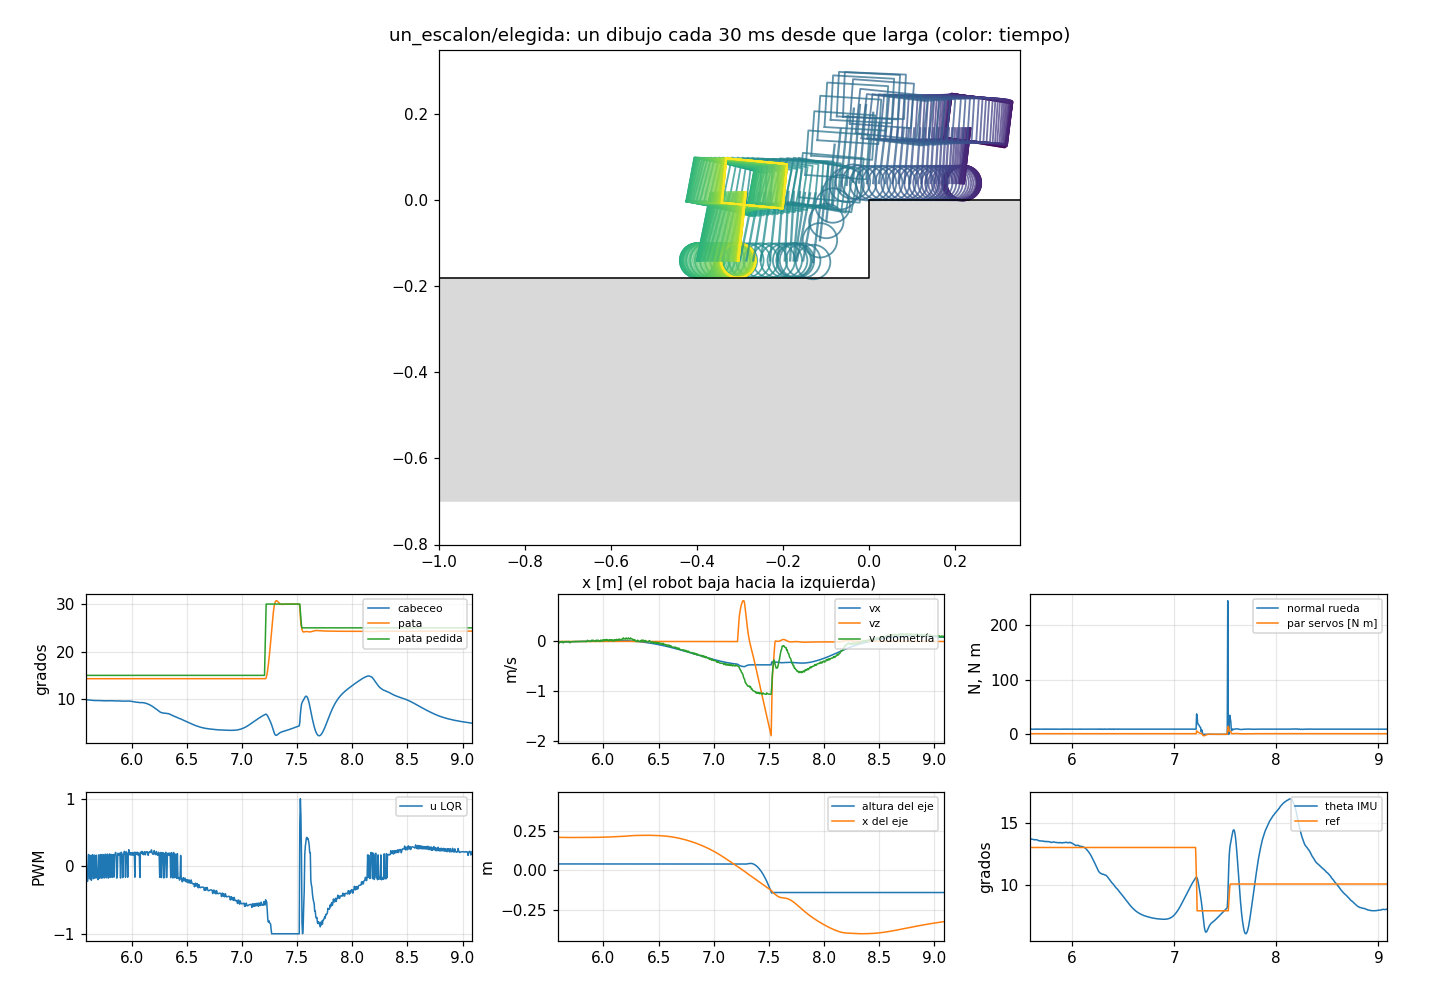
\includegraphics[width=0.95\textwidth]{elegida.png}
\captionof{figure}{Descenso de un escalón de $18\ud{cm}$ con la maniobra por defecto sobre el
modelo ajustado: secuencia cinemática del robot y evolución temporal de ángulos, velocidades y
comandos.}
\end{center}

\begin{center}
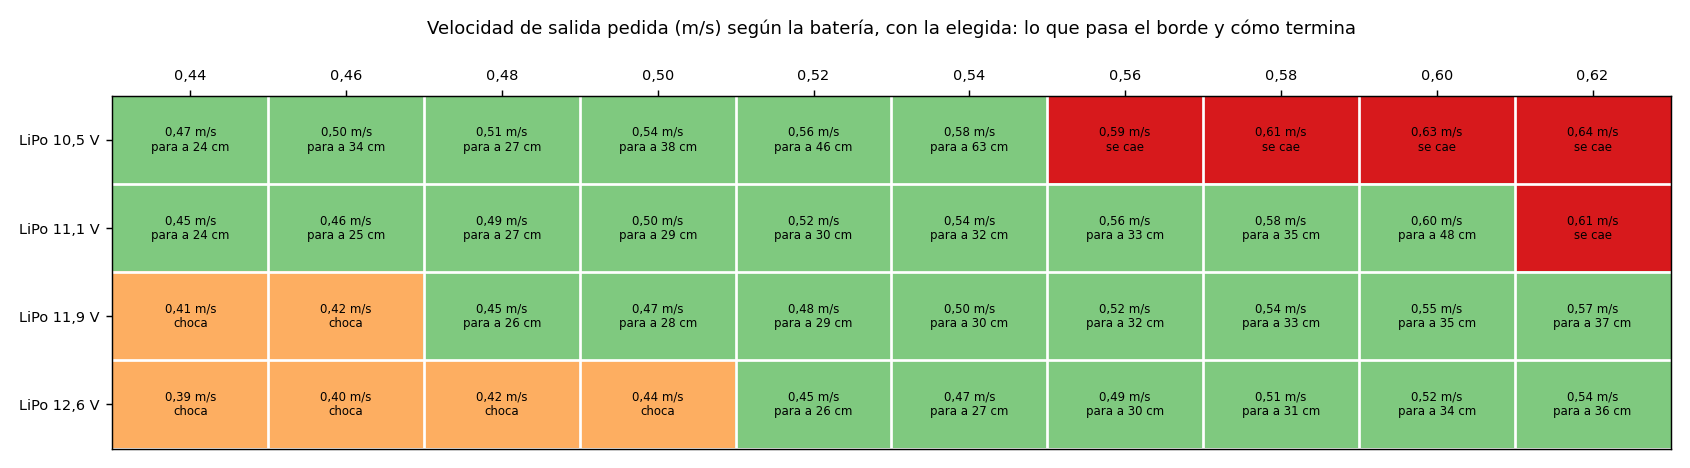
\includegraphics[width=0.82\textwidth]{ventana.png}
\captionof{figure}{Ventana operativa de velocidad de salida para un escalón: por debajo de
$0{,}45\ud{m/s}$ la esquina inferior frontal de la cabina golpea el borde; por encima de
$0{,}58\ud{m/s}$ con batería baja el motor satura en la recepción.}
\end{center}

\section{La escalera real del equipo: por qué no entra frenar en cada escalón}

El objetivo final de maniobra se definió sobre la escalera real medida por el equipo el
3/11/2026: \textbf{6 escalones de 16,6 cm de alto por 29 cm de pisada, seguidos de un séptimo
escalón final de 3 cm}. Se plantearon dos estrategias posibles: bajar \emph{frenando en cada
escalón} (\texttt{repetir = 1}) o bajar \emph{de corrido} (\texttt{t\_continuo}).

El análisis físico y numérico demostró que \textbf{frenar en cada escalón es geométrica y
dinámicamente inviable en una pisada de 29 cm}:
\begin{itemize}[leftmargin=1.5em]
\item Como la cabina sobresale $\sim 9\text{--}10\ud{cm}$ por delante del eje de los servos y el
      robot desciende hacia atrás, la esquina inferior delantera de la cabina es el último punto
      en cruzar la nariz del escalón superior.
\item Para que esa esquina libre el borde sin chocar, el eje de la rueda debe abandonar el
      escalón a una velocidad horizontal mínima de $\approx 0{,}6\text{--}0{,}7\ud{m/s}$.
\item A esa velocidad, tras un vuelo balístico de $\Delta z = 16{,}6\ud{cm}$ ($\approx 185\ud{ms}$),
      las ruedas aterrizan a $13\text{--}14\ud{cm}$ de la contrahuella, dejando apenas
      $\mathbf{15\ud{cm}}$ de pisada restante antes del próximo precipicio. Ninguna ley de
      frenado compatible con el límite de adherencia y el par del motor puede disipar
      $0{,}7\ud{m/s}$ y reacomodar el péndulo invertido en $15\ud{cm}$ (se requieren al menos
      $45\text{--}60\ud{cm}$ de huella).
\end{itemize}

\section{Optimización con algoritmo genético de dos islas (5.300+ corridas)}

En el descenso continuo (\emph{de largo}), el problema cambia de naturaleza: como en $29\ud{cm}$
($\sim 0{,}4\ud{s}$ entre bordes) el péndulo no llega a asentarse en régimen permanente, con
una maniobra ingenua la velocidad crece de escalón en escalón ($0{,}47 \to 0{,}48 \to 0{,}63
\to 1{,}22\ud{m/s}$) hasta que el robot se estrella en el cuarto escalón. Además, en vuelos
sucesivos el LQR en el aire acumula velocidad inversa en las ruedas, por lo que en la escalera
continua resulta indispensable mantener las ruedas girando a la velocidad de salida durante el
vuelo (\texttt{motor\_vuelo = 0}) y disparar acciones sincronizadas con los eventos de
\emph{despegue} y \emph{toque} en cada escalón.

Para hallar una parametrización capaz de estabilizar el ciclo límite escalón tras escalón, se
implementó en \texttt{simulacion/escalon/genetico.py} un \textbf{algoritmo genético de dos islas}
con cromosomas de $18\text{--}20$ genes discretizados a la resolución exacta del firmware
(ángulos de pata de a $1^\circ$, velocidades de a $0{,}01\ud{m/s}$, aceleraciones de a
$0{,}1\ud{m/s^2}$, tiempos de a $0{,}01\ud{s}$ y velocidades de servo de a $10\ud{^\circ/s}$):

\begin{itemize}[leftmargin=1.5em]
\item \textbf{Función de aptitud (\emph{fitness}) multiobjetivo jerárquica:} evalúa primero el
      caso nominal (debe bajar los 7 escalones sin tocar con la cabina y quedar detenido abajo);
      si aprueba, evalúa 5 variaciones filtro y, si supera al menos 4, corre la batería completa
      de \textbf{24 variaciones ponderadas de robustez} (\texttt{variaciones.py}), premiando con
      puntaje máximo aquellos individuos cuya holgura mínima cabina-escalera supere el margen de
      seguridad de $\mathbf{30\ud{mm}}$ pedido por el equipo.
\item \textbf{Resultado tras $> 5.300$ simulaciones ($\sim 50\ud{min}$ de cómputo):} la
      maniobra continua óptima (largada con patas en $10^\circ$, velocidad objetivo $0{,}77\ud{m/s}$
      con rampa de $1{,}2\ud{m/s^2}$, extensión en vuelo a $30^\circ$ a $180\ud{^\circ/s}$ con
      ruedas sostenidas, recepción a $27^\circ$ a $230\ud{^\circ/s}$ retomando $0{,}78\ud{m/s}$
      a $7{,}3\ud{m/s^2}$, y frenado final a $3{,}8\ud{m/s^2}$ tras $0{,}65\ud{s}$ en el llano
      inferior) logra un ciclo periódico estable donde el robot cruza los siete bordes entre
      $\mathbf{0{,}61}$ y $\mathbf{0{,}70\ud{m/s}}$, completando con éxito \textbf{las 24
      variaciones del diseño y las 6 pruebas adicionales de validación ciega}.
\end{itemize}

\begin{center}
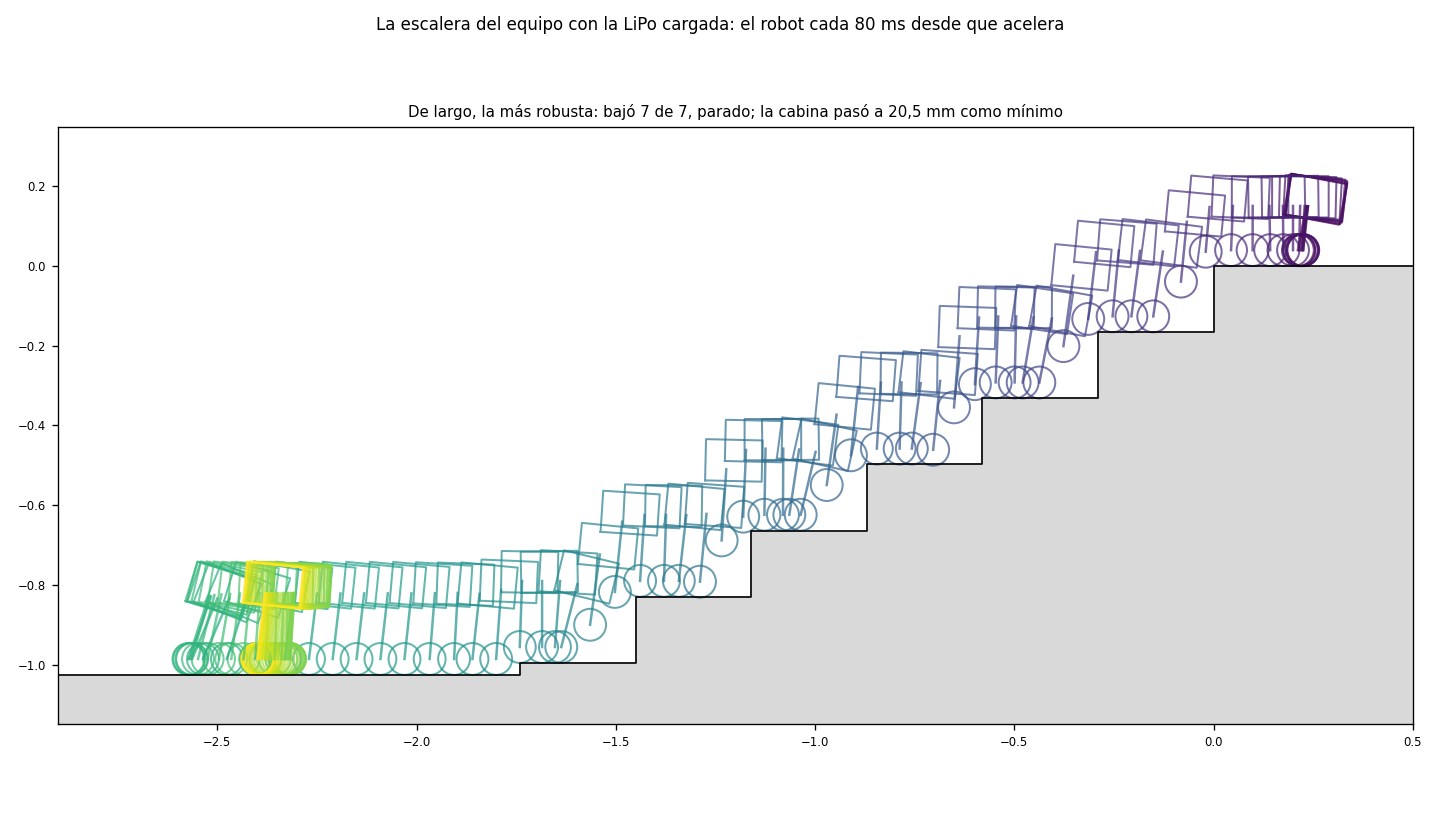
\includegraphics[width=0.98\textwidth]{largo_robusta.png}
\captionof{figure}{Maniobra continua más robusta hallada por el algoritmo genético descendiendo
los 7 escalones de la escalera real del equipo ($6 \times 16{,}6\ud{cm} + 1 \times 3\ud{cm}$) y
frenando en el descanso inferior.}
\end{center}

\begin{center}
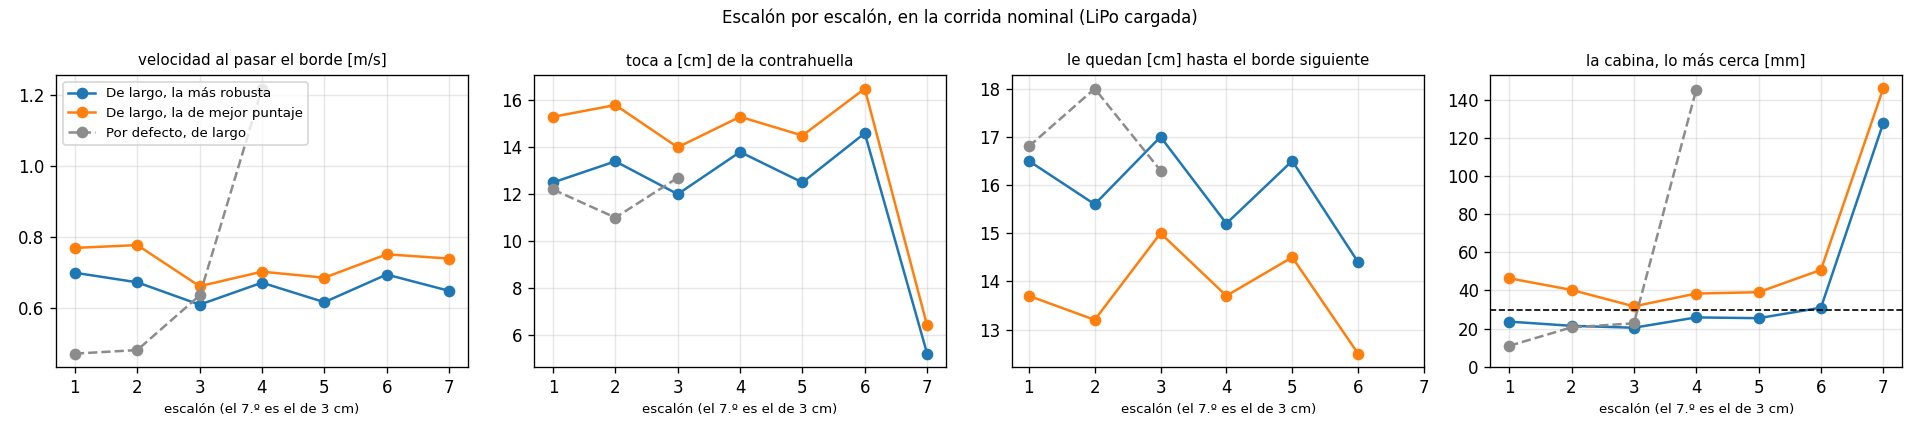
\includegraphics[width=0.92\textwidth]{por_escalon.png}
\captionof{figure}{Estabilidad del ciclo límite escalón por escalón: velocidad en el borde,
punto de aterrizaje sobre la huella de $29\ud{cm}$ y holgura mínima de la cabina.}
\end{center}

\section{Compromiso geométrico de holgura y recorte frontal de la cabina}

El análisis de sensibilidad geométrica (\texttt{escalera\_real.py}, figura \ref{fig:cambios_esc})
reveló el último resultado clave para el diseño mecánico: con el contorno original de la cabina,
la maniobra más robusta (que acierta 24/24 variaciones) pasa con la esquina inferior delantera
a entre $\mathbf{17\text{ y }27\ud{mm}}$ de la nariz del escalón (mediana $21\ud{mm}$). Si se
exige al algoritmo genético alcanzar los $30\ud{mm}$ de holgura sin tocar el CAD, el optimizador
se ve forzado a subir la velocidad de salida a $0{,}81\ud{m/s}$, perdiendo robustez (falla en
4 de las 24 variaciones). En cambio, \textbf{recortando o achaflanando apenas $2\ud{cm}$ la
arista inferior delantera de la cabina}, la misma maniobra robusta de $0{,}77\ud{m/s}$ supera los
$\mathbf{35\ud{mm}}$ de holgura en las 24 variaciones sin sacrificar margen de estabilidad.

\begin{center}
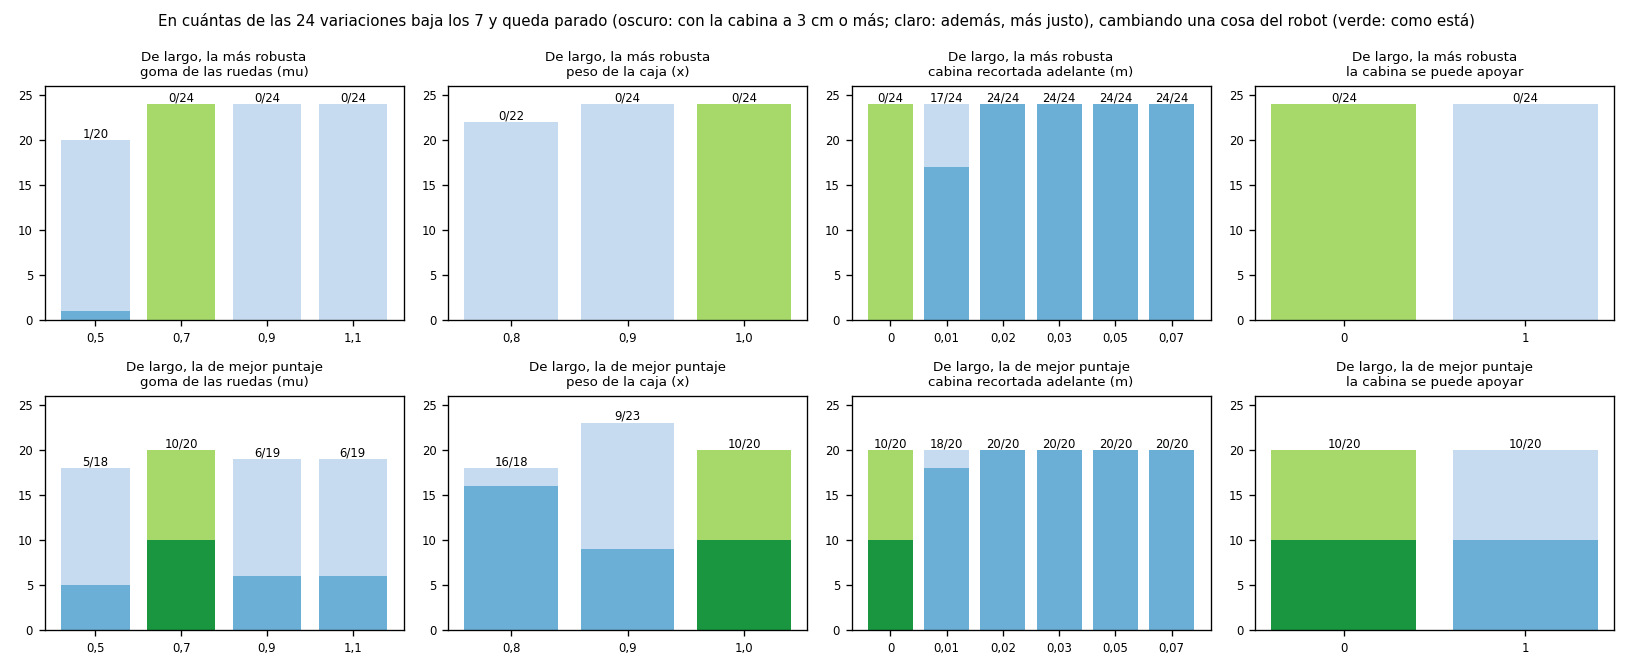
\includegraphics[width=0.88\textwidth]{cambios.png}
\captionof{figure}{Estudio de sensibilidad constructiva sobre la escalera real: efecto de
recortar $1\ud{cm}$ o $2\ud{cm}$ el frente de la cabina, variar el coeficiente de fricción del
neumático y reducir un $20\%$ la masa de la caja.}\label{fig:cambios_esc}
\end{center}

Finalmente, todas las herramientas desarrolladas convergen en el visor web interactivo
(\texttt{simulacion/escalon/visor/visor.py}) y en el script de contraste experimental
\texttt{comparar\_prueba.py}, que superpone la telemetría grabada a $200\ud{Hz}$ durante una
bajada real del robot contra la predicción del banco híbrido (figura \ref{fig:bajada_real}).

\begin{center}
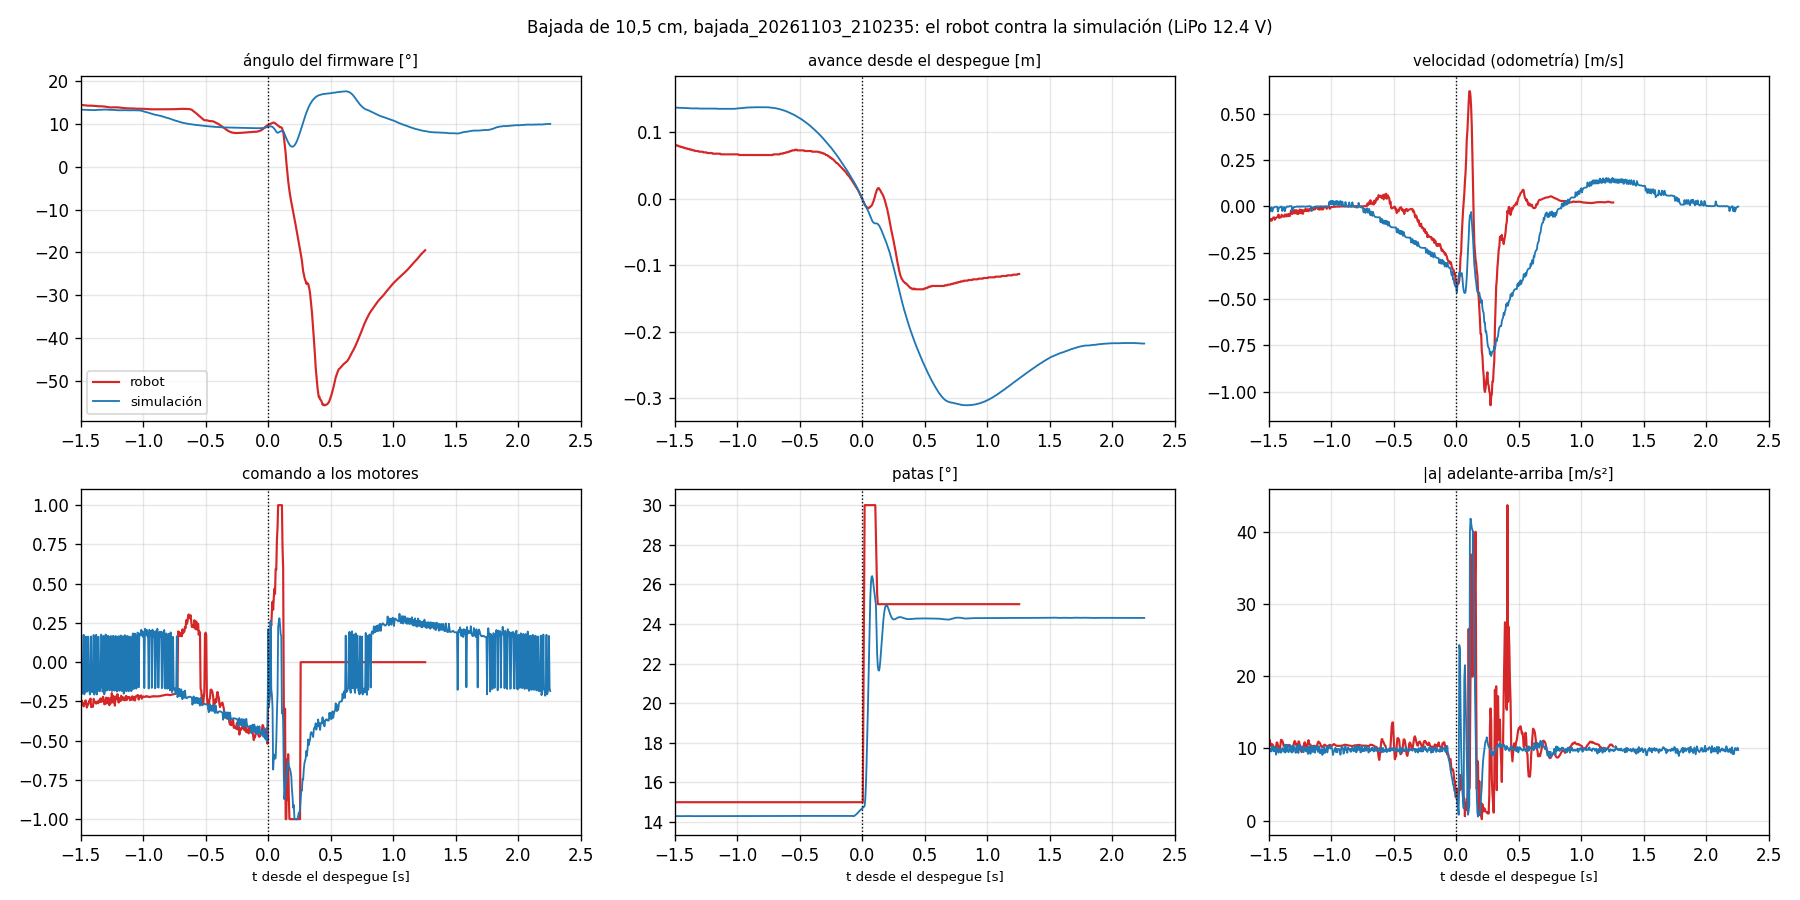
\includegraphics[width=0.95\textwidth]{bajada_20261103_210235.png}
\captionof{figure}{Registro experimental a $200\ud{Hz}$ de una prueba de bajada en el prototipo
(\texttt{bajada\_20261103\_210235.csv}) contrastado automáticamente contra la simulación del
banco en C.}\label{fig:bajada_real}
\end{center}


% ===========================================================================
\chapter{Conclusiones técnicas y lecciones de ingeniería}\label{cap:concl}
% ===========================================================================

\begin{idea}
El diseño basado en modelo permitió anticipar comportamientos físicos no intuitivos, dimensionar
actuadores sin sobredimensionar la masa total ($962\ud{g}$) y, cuando el robot real se apartó
del CAD nominal, identificar con pocos ensayos qué parámetros estaban mal y cuánto.
\end{idea}

\section{Síntesis de hallazgos físicos y de control}

\begin{enumerate}[leftmargin=1.6em]
\item \textbf{Dominio de la inercia baricéntrica sobre el efecto péndulo:} duplicar la altura del
      centro de masa (de $7{,}9$ a $15{,}8\ud{cm}$) varía el polo inestable apenas un $7\%$
      ($6{,}91$ a $7{,}43\ud{s^{-1}}$), porque la inercia rotacional propia de la cabina y las
      patas domina frente a $m\ell^2$. En consecuencia, las patas no están para facilitar el
      equilibrio, sino para aportar despeje geométrico y actuar como suspensión activa en el
      aterrizaje.
\item \textbf{Amortiguamiento electromagnético dominante:} la fuerza contraelectromotriz del
      motorreductor GA25-370 aporta un amortiguamiento viscoso reflejado cien veces superior al
      rozamiento mecánico y baja el polo inestable de $\approx 13\ud{s^{-1}}$ a
      $7{,}35\ud{s^{-1}}$: el tiempo en que se duplica la inclinación pasa de $\sim 53$ a
      $\sim 94\ud{ms}$.
\item \textbf{Fuerza real en el contacto vs.\ $\tau/r$:} al acelerar, gran parte del par del
      motor se invierte en acelerar angularmente el rotor multiplicado por $N^2$ y la propia
      rueda; la fuerza horizontal que exige adherencia al suelo es el $87\text{--}94\%$ del
      límite de Coulomb ($\mu = 0{,}7$), dejando a motor y neumático prácticamente empatados.
\item \textbf{Límite de linealización gobernado por el coseno del acople:} en las ecuaciones de
      Euler-Lagrange, la aproximación $\cos\varphi \approx 1$ en el término inercial cruzado
      introduce un error de orden $\mathcal{O}(\varphi^2)$, rompiendo la aproximación lineal
      mucho antes que $\sin\varphi \approx \varphi$, que falla recién a orden $\mathcal{O}(\varphi^3)$.
\item \textbf{Cierre del ciclo Teoría--Experimento--Control:} la arquitectura de software con el
      núcleo de control en C puro permitió que exactamente las mismas funciones corrieran en el
      ESP32-S3 a $200\ud{Hz}$, en el banco de identificación experimental y en las más de $5.300$
      corridas del algoritmo genético, garantizando trazabilidad directa entre simulación y
      prototipo físico.
\end{enumerate}

% ===========================================================================
\appendix
\chapter{Cinemática de la pata: desarrollo completo}\label{ap:cin}
% ===========================================================================
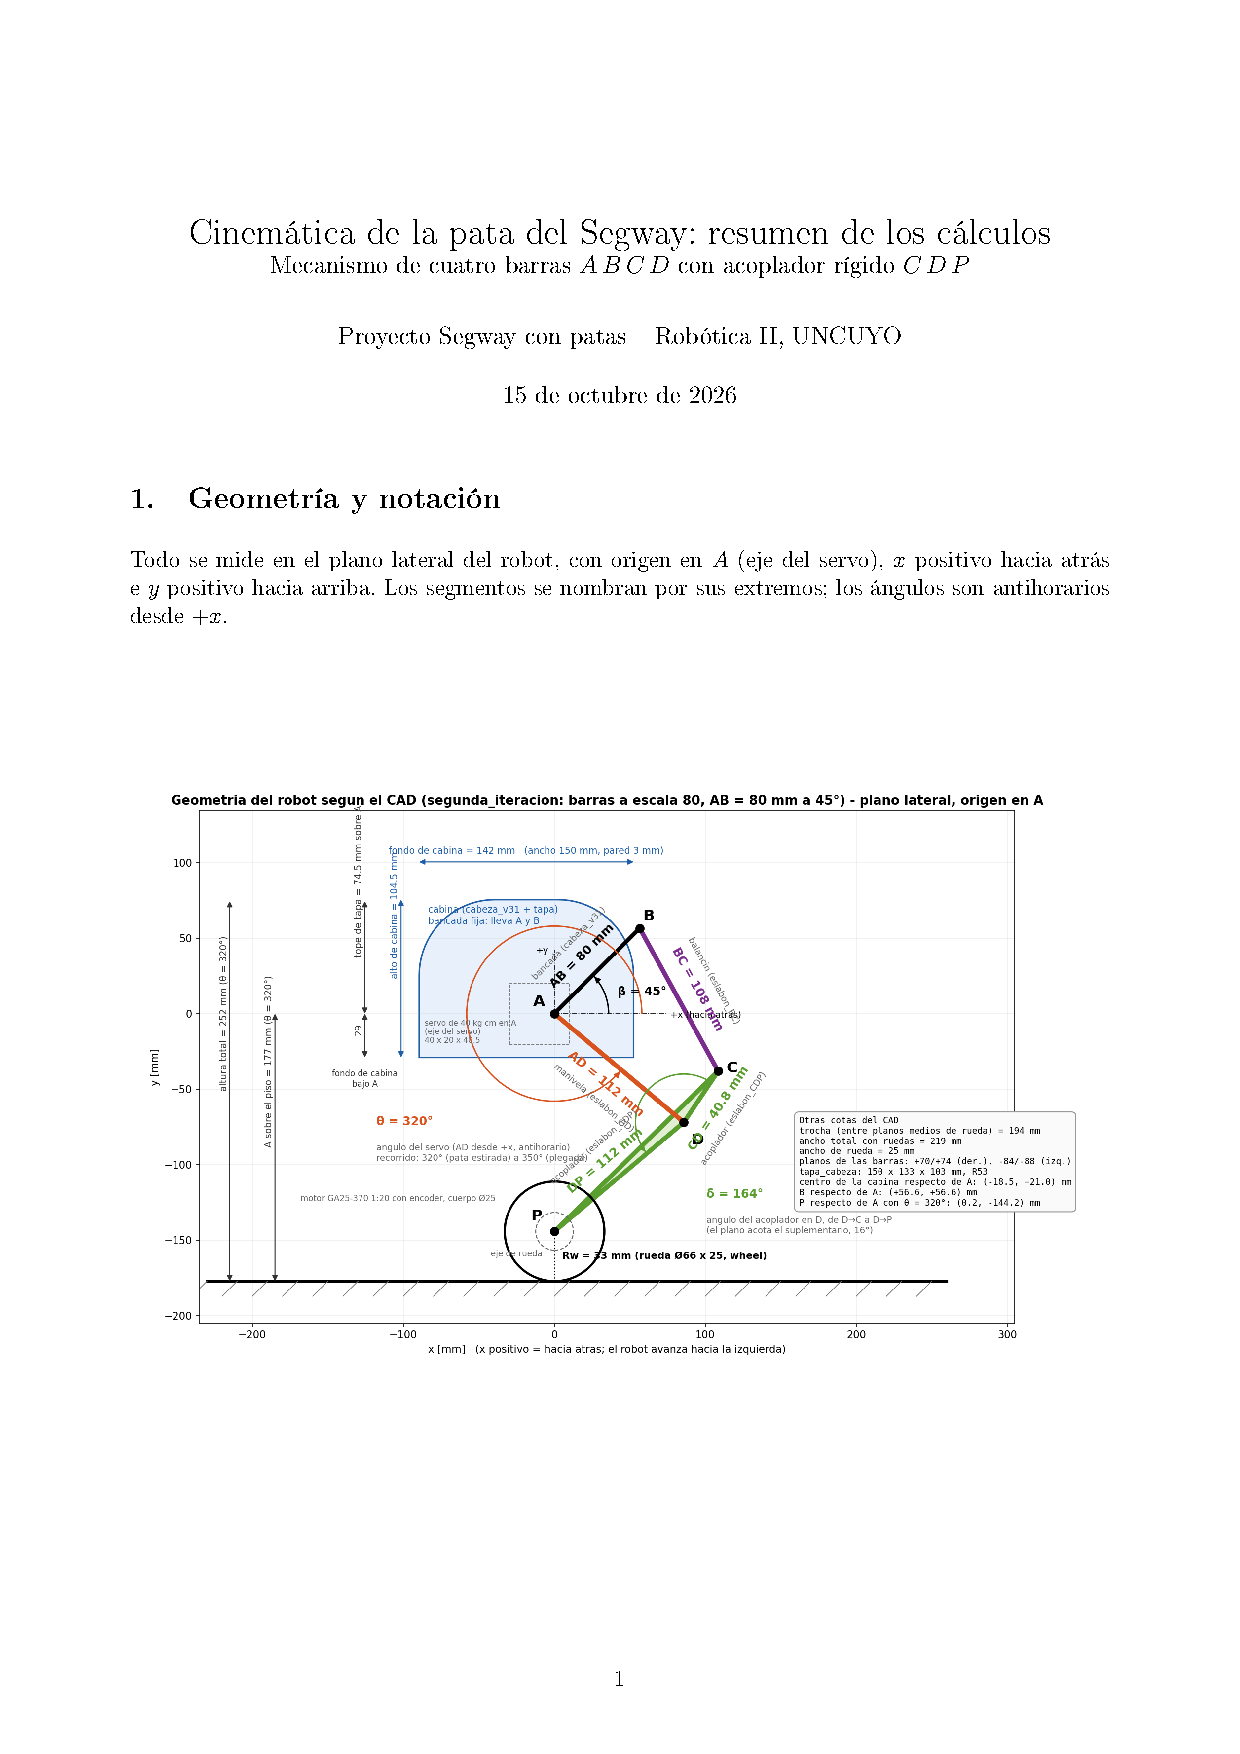
\includepdf[pages=-,scale=0.92,pagecommand={}]{../modelado/cinematica/cinematica_resumen.pdf}

\chapter{Diagramas de cuerpo libre}\label{ap:dcl}
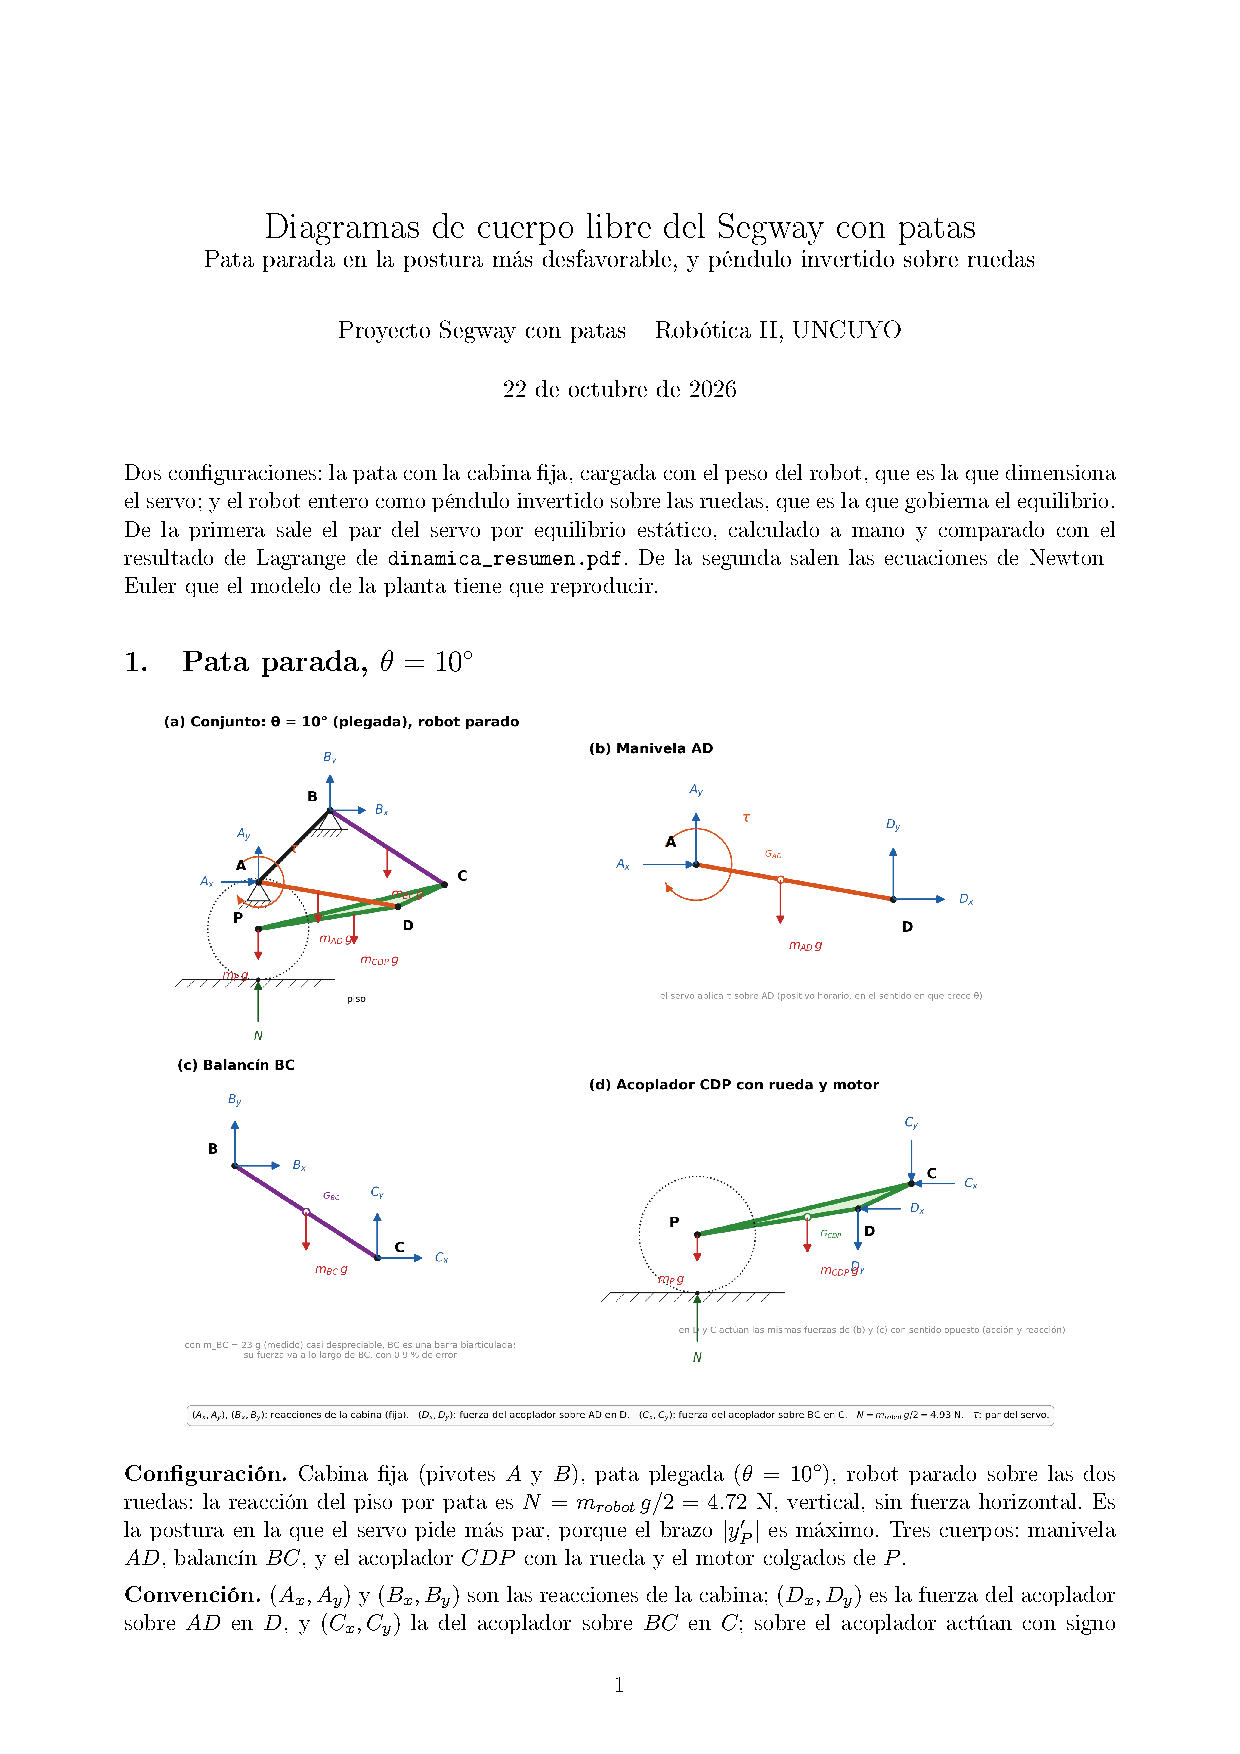
\includepdf[pages=-,scale=0.92,pagecommand={}]{../modelado/dcl/dcl_resumen.pdf}

\chapter{Dinámica de la pata por Lagrange}\label{ap:dinres}
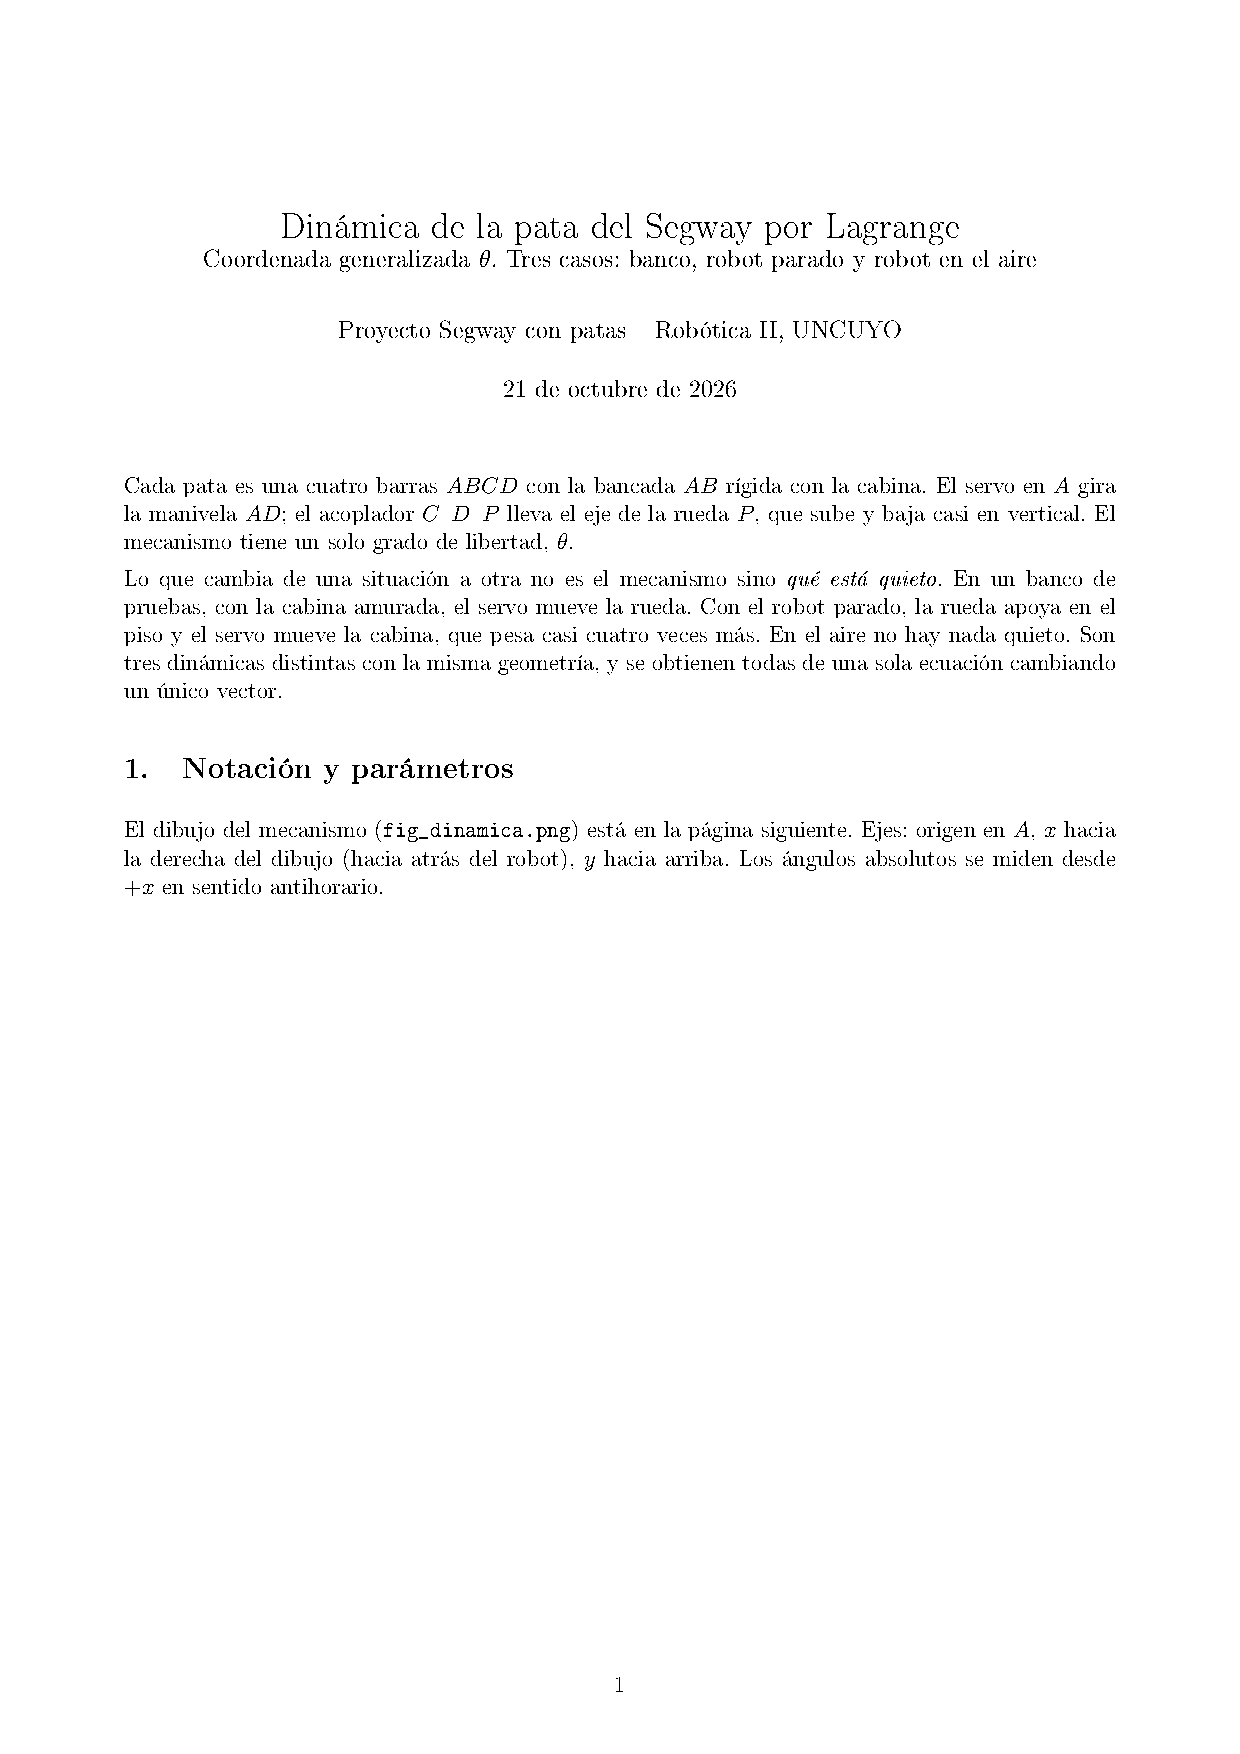
\includepdf[pages=-,scale=0.92,pagecommand={}]{../modelado/dinamica/dinamica_resumen.pdf}

\chapter{Dinámica de la pata con el robot apoyado}\label{ap:dinapo}
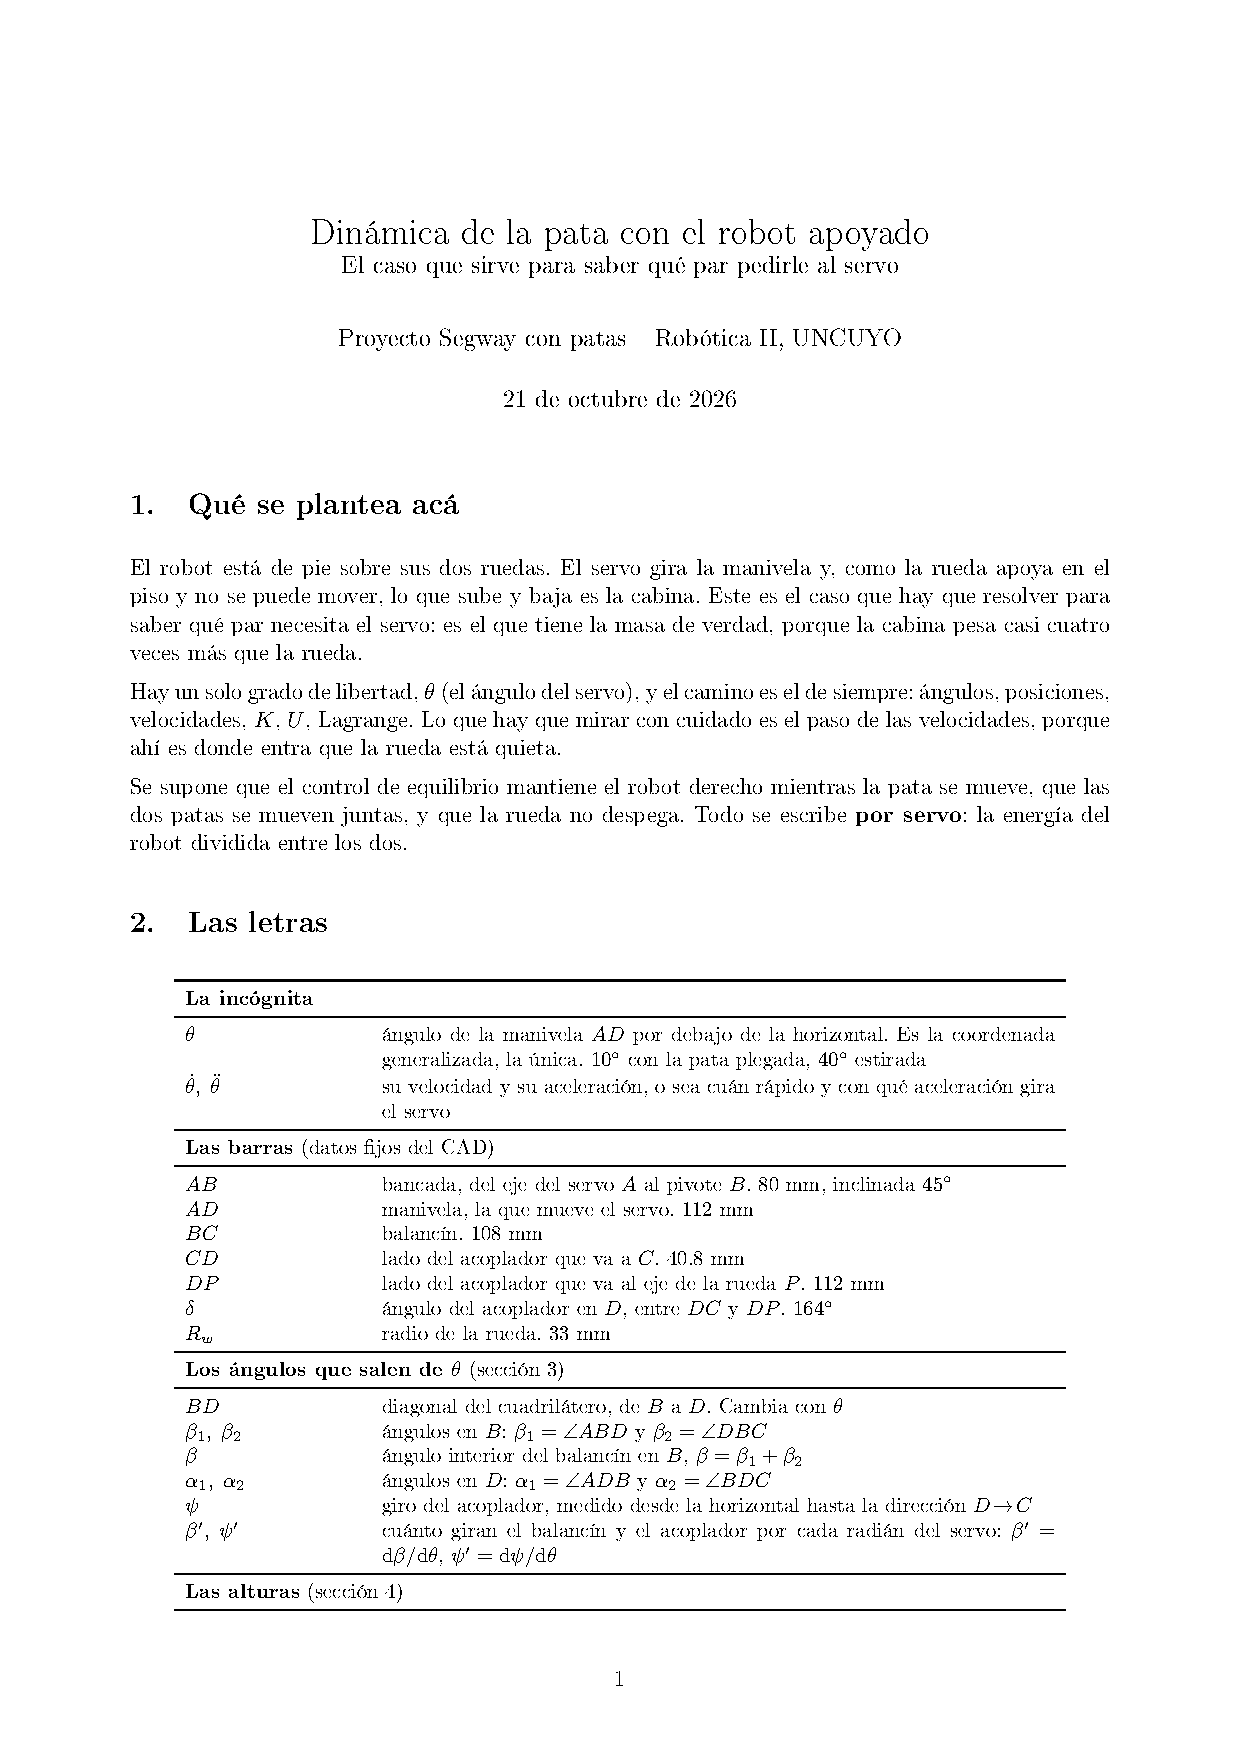
\includepdf[pages=-,scale=0.92,pagecommand={}]{../modelado/dinamica/dinamica_apoyado.pdf}

\chapter{Documentación constructiva de las placas electrónicas (Potencia v0.7 y Lógica v0.6)}\label{ap:pcb}
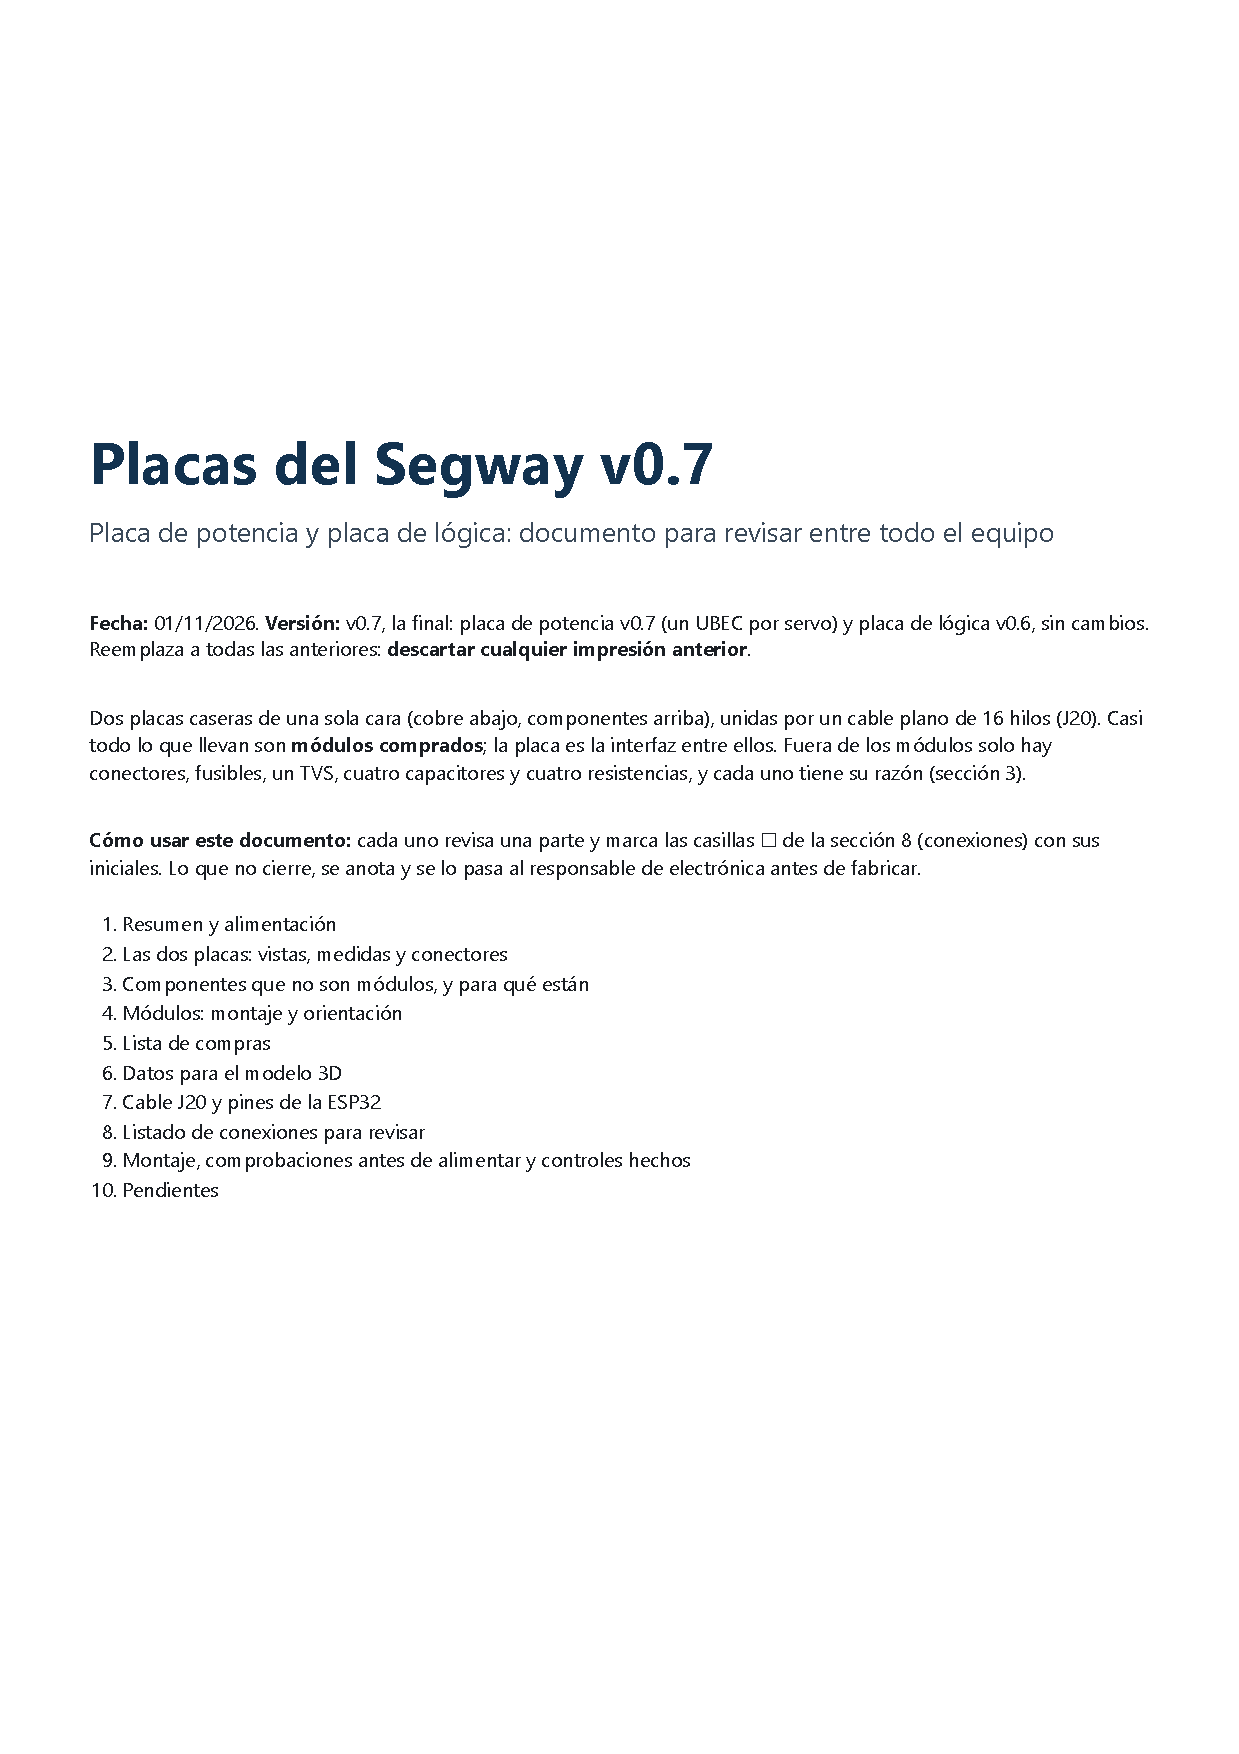
\includepdf[pages=-,scale=0.92,pagecommand={}]{../docs/placas_v0.7_completo.pdf}

\end{document}
